\chapter{Resultados Obtidos}
Este capítulo demonstra os artefatos produzidos para o \textit{software}, incluindo 
as informações associadas desde a análise até os testes.

% ----------------------------------------------------------
\section{Diagnóstico do Processo Atual} \label{chapter:diagnostico}
% ----------------------------------------------------------
% MARCELO 17/05: esse capítulo é um resultado das entrevistas, sendo utilizado para a construção dos requisitos. 
% Pode unir como seção no próximo capítulo
% VITOR 20/05: OK
\subsection{Visão Geral do Processo Atual}

Com base em informações obtidas através de entrevistas e conversar com os profissionais do CECLIMAR, foi possível 
identificar e mapear o processo atual de coleta e registro de dados da fauna marinha no litoral do Rio Grande do Sul.

Hoje, o CECLIMAR realiza o monitoramento da fauna costeira por meio de registros enviados pela comunidade, 
por pesquisadores em campo e por profissionais do Corpo de Bombeiros Militar. O processo 
ocorre de forma manual, como ilustrado na Figura~\ref{fig:fluxo_detalhado}. Esta abordagem envolve 
diversas etapas intermediárias e tarefas manuais realizadas por diferentes profissionais, trazendo
uma maior probabilidade de erros e inconsistências nos dados coletados, além de aumentar o tempo
de processamento e análise das informações.

\subsection{Descrição do Fluxo de Trabalho Atual}

O fluxo de trabalho pode ser descrito em etapas principais:

\begin{enumerate}
    \item \textbf{Envio de dados:} Os participantes enviam fotos e informações descritivas a partir de diversas fontes.
    \item \textbf{Triagem inicial:} Um pesquisador analisa as mensagens recebidas por meio de análise manual em cada uma das fontes e seleciona os dados relevantes.
    \item \textbf{Registro:} A bolsista transcreve os dados válidos para uma planilha eletrônica.
    \item \textbf{Armazenamento de imagens:} As fotos dos registros são manualmente salvas em uma pasta no Google Drive com o id do registro na tabela.
    \item \textbf{Validação:} O gestor revisa periodicamente os dados para verificar consistências e erros.
\end{enumerate}

A Figura~\ref{fig:fluxo_detalhado} apresenta o fluxo de trabalho atual de maneira esquemática, 
destacando as principais etapas e interações entre os envolvidos no processo de coleta e registro de dados.
Como é possível ver na Tabela~\ref{tab:contagem_ocorrencias}, atualmente, a maioria (48,45\%) dos dados 
é coletada via \citeonline{whatsApp}, mas esses envios também ocorrem por outras plataformas 
como ligações telefônicas, \citeonline{facebook2025}, e-mail, e \citeonline{instagram2025}.

\begin{table}[h]
    \centering
    \begin{tabular}{|l|c|c|}
    \hline
    \textbf{Canal}     & \textbf{Quantidade} & \textbf{Porcentagem} \\
    \hline
    Ligação     & 860  & 21,52\% \\
    E-mail       & 343  & 8,59\%  \\
    Facebook    & 703  & 17,60\% \\
    WhatsApp    & 1935 & 48,45\% \\
    Instagram   & 153  & 3,83\%  \\
    \hline
    \textbf{Total}     & 3994 & 100\% \\
    \hline
    \end{tabular}
    \caption{Contagem e porcentagem de ocorrências por canal de comunicação}
    \label{tab:contagem_ocorrencias}
    \legend{Fonte: Autor}
\end{table}

\begin{figure}[H]
    \centering
    \begin{tikzpicture}[node distance=1cm]
    
    \tikzstyle{startstop} = [rectangle, rounded corners, minimum width=3.5cm, minimum height=1cm,text centered, draw=black, fill=red!30]
    \tikzstyle{input} = [rectangle, minimum width=3.5cm, minimum height=1cm, text centered, draw=black, fill=yellow!30]
    \tikzstyle{process} = [rectangle, minimum width=3.5cm, minimum height=1cm, text centered, draw=black, fill=blue!30]
    \tikzstyle{storage} = [rectangle, minimum width=3.5cm, minimum height=1cm, text centered, draw=black, fill=purple!30]
    \tikzstyle{decision} = [diamond, minimum width=3cm, minimum height=1cm, text centered, draw=black, fill=green!30]
    \tikzstyle{arrow} = [thick,->,>=stealth]
    
    \node (whatsapp) [input] {WhatsApp};
    \node (email) [input, below left=1cm of whatsapp] {Email};
    \node (instagram) [input, below=1.2cm of email] {Instagram};
    \node (facebook) [input, below right=1cm of whatsapp] {Facebook};
    \node (call) [input, below=1.2cm of facebook] {Ligação};
    
    \node (triage) [process, below=4.3cm of whatsapp] {Triagem por Pesquisador};
    
    \node (valid) [decision, below=1.2cm of triage] {Dados válidos?};
    
    \node (discard) [startstop, right=2cm of valid] {Descartar Registro};
    \node (refactor) [startstop, left=2cm of valid] {Reestruturar Registro};
    
    \node (record) [process, below=1cm of valid] {Registro em Planilha (Bolsista)};
    \node (storage) [storage, below=1cm of record] {Armazenamento de Fotos (Google Drive)};
    \node (review) [process, below=1cm of storage] {Validação periódica (Gestor)};

    \draw [arrow] (whatsapp) -- (triage);
    \draw [arrow] (email) -- (triage);
    \draw [arrow] (instagram) -- (triage);
    \draw [arrow] (facebook) -- (triage);
    \draw [arrow] (call) -- (triage);
    
    \draw [arrow] (triage) -- (valid);
    \draw [arrow] (valid) -- node[above] {Não} (discard);
    \draw [arrow] (valid) -- node[above] {Não} (refactor);
    \draw [arrow] (valid) -- node[right] {Sim} (record);
    \draw [arrow] (record) -- (storage);
    \draw [arrow] (storage) -- (review);
    \draw [arrow] (refactor) -- (record);
    \draw [arrow, bend right=45] (review.east) to (valid.east);

    \end{tikzpicture}
    \caption{Fluxograma detalhado do processo atual de coleta e registro de dados no CECLIMAR.}
    \legend{Fonte: Autor}
    \label{fig:fluxo_detalhado}
\end{figure}
    
\subsection{Problemas Identificados}

Os principais problemas observados neste fluxo incluem:

\begin{itemize}
    \item Risco de erros humanos durante transcrição dos dados.
    
    \item Dificuldade de padronização nas descrições enviadas.
    \begin{itemize}
        \item Para que a tabela automatizada funcione, os dados precisam estar exatamente iguais.
        \item Erros de digitação na taxônomia dos animais.
        \item Problemas com formatações de campos.
    \end{itemize}
    
    \item Atraso no tempo de registro e análise das ocorrências.
    
    \item Necessidade de revisões periódicas para manter a qualidade dos dados.
    
    \item Falta de integração entre os dados (planilha e fotos separadas).
    
    \item Necessidade de acesso a múltiplas fontes para avaliar os registros.
    
    \item Pouca visibilidade da participação da comunidade no projeto.
\end{itemize}


\section{Levantamento de Requisitos}

O levantamento de requisitos foi essencial para compreender as necessidades do projeto e orientar o 
desenvolvimento das funcionalidades do aplicativo. Segundo 
\citeonline{sommerville2011}, os requisitos de um sistema são as descrições do que o sistema deve 
fazer, os serviços que ele irá oferecer e suas restrições de funcionamento. Neste projeto, a 
definição dos requisitos prioritários para o MVP\footnote{MVP é a sigla para 
\textit{Minimum Viable Product} (Produto Mínimo Viável), um conceito que se refere à 
versão mais simples de um produto 
que ainda entrega valor ao usuário e permite validações com o mínimo de esforço e 
custo.} e das suas limitações foi orientada por reuniões 
com o coordenador do projeto Fauna Marinha RS, especialmente com base na experiência prática dos 
profissionais do CECLIMAR, que indicaram as funcionalidades mais relevantes para o sistema.

\subsection{Requisitos Funcionais}

Nesta seção, serão expostos os requisitos funcionais do sistema, que segundo 
\citeonline{guedesuml2} correspondem ao que o cliente quer que o sistema realize,
ou seja, as funcionalidades do software. Esses requisitos estão organizados em tabelas
distintas, apresentadas a seguir. A Tabela~\ref{tab:req-funcionais} sintetiza os 63 requisitos funcionais
da versão 2.3.6 do aplicativo, que é a versão mais atualizada até o momento da entrega deste relatório.
Durante o desenvolvimento, os requisitos foram revisados e atualizados conforme necessário,
com base em feedbacks e testes realizados.

\begin{longtable}{@{}p{1.5cm}p{13cm}@{}}
    \caption{Requisitos funcionais do sistema}\label{tab:req-funcionais}\\
        \toprule
        \textbf{Código} & \textbf{Descrição} \\ \hline
        \midrule
        \endfirsthead
        
        \toprule
        \textbf{Código} & \textbf{Descrição} \\ \hline
        \midrule
        \endhead
        
        \midrule
        \multicolumn{2}{r@{}}{(Continua na próxima página)} \\
        \endfoot
        
        \bottomrule
        \endlastfoot
    % usuario
    % registro
    RF01 & O sistema deve permitir o registro de novos usuários com e-mail e senha. \\ \hline
    RF02 & O sistema deve permitir o registro de novos usuários com conta Google integrada ao Firebase Authentication. \\ \hline
    RF03 & O sistema deve diferenciar dois tipos de usuários: cientista cidadão (user) e pesquisador (admin). \\ \hline
    RF04 & O sistema deve permitir que um pesquisador cadastre outro pesquisador, com geração automática de senha segura (8 dígitos alfanuméricos e caracteres especiais). \\ \hline
    RF05 & O sistema deve permitir que um pesquisador conceda a outro usuário que já possui conta a role de pesquisador. \\ \hline

    % login
    RF06 & O sistema deve permitir o login via Firebase Authentication com e-mail e senha. \\ \hline
    RF07 & O sistema deve permitir o login via conta Google integrada ao Firebase Authentication. \\ \hline
    RF08 & O sistema deve unificar dados quando uma conta possui ambos os métodos de login. \\ \hline
    RF09 & O sistema deve permitir redefinição de senha através do fluxo do Firebase Authentication (envio de e-mail de redefinição). \\ \hline
    RF10 & O sistema deve permitir a recuperação da senha. \\ \hline
    RF11 & O sistema deve permitir que o usuário faça logoff. \\ \hline

    % exclusao de conta
    RF12 & O sistema deve permitir a exclusão da conta do usuário, independente do método de cadastro. \\ \hline
    RF13 & O sistema deve manter os registros realizados pelo usuário mesmo após a exclusão da conta, 
    para preservação de dados científicos. \\ \hline

    % editar perfil
    RF14 & O sistema deve permitir atualização do perfil de usuário cadastrado com e-mail e senha (nome, foto, e-mail). \\ \hline
    
    % tela de meu perfil
    RF15 & O sistema deve permitir ao usuário visualizar e gerenciar seu perfil. \\ \hline
    RF16 & O sistema deve possuir um conjunto de conquistas para cada usuário. \\ \hline
    RF17 & O sistema deve permitir ao usuário visualizar os últimos registros do seu perfil. \\ \hline
    RF18 & O sistema deve permitir ao usuário visualizar a quantidade total de registros realizadas por ele. \\ \hline

    % envio de registros
    RF19 & O sistema deve permitir envio de registros "simples". \\ \hline
    RF20 & O sistema deve permitir envio de registros "técnicos" com dados mais específicos. \\ \hline
    RF21 & O sistema deve permitir envio de até 2 imagens por registro, sendo uma obrigatória. \\ \hline
    RF22 & O sistema deve permitir envio de registros utilizando GPS do dispositivo em tempo real para obter as coordenadas geográficas. \\ \hline
    RF23 & O sistema deve validar os formulários de envio de registros com restrições específicas (ex.: limite de caracteres). \\ \hline
    RF24 & O sistema deve permitir que o usuário envie uma imagem a partir da galeria do celular. \\ \hline
    RF25 & O sistema deve permitir que o usuário envie uma imagem a partir da camera do celular. \\ \hline
    RF26 & O sistema deve permitir consultar dados de geolocalização a partir das. \\ \hline
    RF27 & O sistema deve permitir envio de registros utilizando a opção número da guarita para basear as coordenadas geográficas. \\ \hline
    RF28 & O sistema deve permitir envio de registros utilizando coordenadas da cidade para definir a localização. \\ \hline
    RF29 & O sistema deve permitir envio de registros utilizando ponto de referência como campo aberto. \\ \hline
    RF30 & O sistema deve facilitar a ativação da geolocalização do dispositivo pelo usuário. \\ \hline
    RF31 & O sistema deve permitir visualizar a imagem de um registro em tela cheia. \\ \hline
    RF32 & O sistema deve exibir o nome da cidade automaticamente com base na localização do registro. \\ \hline
    RF33 & O sistema deve permitir o armazenamento de registros quando enviados offline. \\ \hline

    %sobre 
    RF34 & O sistema deve apresentar uma tela com informações sobre o projeto e os desenvolvedores. \\ \hline

    % meus registros
    RF35 & O sistema deve permitir que o usuário visualize todos registros que ele enviou. \\ \hline
    RF36 & O sistema deve permitir que o usuário filtre os registros enviados e já validados. \\ \hline
    RF37 & O sistema deve permitir que o usuário receba o retorno do profissional para cada registro. \\ \hline
    RF38 & O sistema deve permitir que um pesquisador delete um registro enviado por qualquer usuário. \\ \hline
    RF39 & O sistema deve permitir a visualização detalhada de um registro selecionado. \\ \hline
    
    % interface
    RF40 & O sistema deve apresentar uma barra de navegação fixa com as opções: início, registros, 
    novo registro, perfil e sobre. \\ \hline
    RF41 & O sistema deve apresentar um menu inicial com todas as funcionalidades disponíveis. \\ \hline
    RF42 & O sistema deve assegurar que apenas usuários pesquisadores tenham acesso a algumas funcionalidades. \\ \hline
    RF43 & O sistema deve possuir uma seção para apresentar os principais animais da fauna local. \\ \hline
    RF44 & O sistema deve possuir uma tela de carregamento inicial. \\ \hline

    % painel de registros
    RF45 & O sistema deve permitir que o usuário visualize os registros enviados por outros usuários. \\ \hline
    RF46 & O sistema deve disponibilizar um painel de registros com estatísticas, mapas e filtros detalhados para acompanhamento. \\ \hline
    RF47 & O sistema deve permitir que os usuários comuns exportem um arquivo CSV com dados sensíveis ocultos. \\ \hline
    RF48 & O sistema deve permitir que os pesquisadores exportem um arquivo CSV com os dados gerais dos registros. \\ \hline
    RF49 & O sistema deve permitir que sejam vistos todos os registros enviados ainda não avaliados. \\ \hline
    RF50 & O sistema deve permitir que sejam vistos todos os registros já avaliados. \\ \hline
    RF51 & O sistema deve apresentar um mapa interativo com pontos de registros. \\ \hline
    RF52 & O sistema deve apresentar os animais que possuem mais registros documentados. \\ \hline
    RF53 & O sistema deve incrementar o número de encontros com cada espécie após uma avaliação de pesquisador. \\ \hline
    RF54 & O sistema deve possuir um contador por classe para os mamíferos, as aves e os répteis. \\ \hline
    RF55 & O sistema deve permitir a busca de registros por espécie. \\ \hline
    RF56 & O sistema deve permitir a busca de número de registros dentro de uma faixa de tempo. \\ \hline

    % avaliacao de registros
    RF57 & O sistema deve permitir que pesquisadores avaliem de todos os registros enviados. \\ \hline
    RF58 & O sistema deve permitir a inserção de novos animais no banco de dados. \\ \hline
    RF59 & O sistema deve permitir que o pesquisador adicione comentários aos registros enviados. \\ \hline
    RF60 & O sistema deve permitir que os dados enviados por um usuário sejam editáveis para um pesquisador realizar
    a avaliação. \\ \hline
    RF61 & O sistema deve permitir ao pesquisador atualizar a localização ao avaliar um registro. \\ \hline

    % fauna local
    RF62 & O sistema deve redirecionar para o site do projeto Fauna Marinha RS para dados da fauna local. \\ \hline
    RF63 & O sistema deve redirecionar para as redes sociais do projeto Fauna Marinha RS. \\ \hline
\end{longtable}
\legend{Fonte: Autor}

\subsection{Requisitos Não Funcionais}

Segundo \citeonline{pressman2011engenharia}, os requisitos não funcionais podem ser descritos 
como uma característica de qualidade, desempenho, segurança ou restrição geral de um sistema. 
Na Tabela~\ref{tab:req-nao-funcionais}, temos o detalhamento desses requisitos, com a finalidade 
de sintetizar as propriedades essenciais que asseguram o bom funcionamento da aplicação. 
Tais requisitos são fundamentais 
para garantir aspectos como usabilidade, confiabilidade, portabilidade e eficiência, além de assegurar 
conformidade com as tecnologias e práticas adotadas no desenvolvimento do sistema.

\begin{longtable}{@{}p{1.5cm}p{13cm}@{}}
    \caption{Requisitos não funcionais do sistema}\label{tab:req-nao-funcionais}\\
    \toprule
    \textbf{Código} & \textbf{Descrição} \\ \hline
    \midrule
    \endfirsthead
    
    \toprule
    \textbf{Código} & \textbf{Descrição} \\ \hline
    \midrule
    \endhead
    
    \midrule
    \multicolumn{2}{r@{}}{(Continua na próxima página)} \\
    \endfoot
    
    \bottomrule
    \endlastfoot
    RNF01 & O sistema deve ser desenvolvido utilizando Flutter e Dart, garantindo compatibilidade 
    multiplataforma. \\ \hline
    RNF02 & O sistema deve utilizar autenticação segura via Firebase, com criptografia adequada para 
    senhas e tokens. \\ \hline
    RNF03 & O sistema deve apresentar alta disponibilidade e ser resiliente a falhas de rede. \\ \hline
    RNF04 & O sistema deve indicar quando alguma funcionalidade não está disponível. \\ \hline
    RNF05 & O sistema deve seguir as melhores práticas de UX, com validação clara de formulários e 
    feedbacks visuais para os usuários. \\ \hline
    RNF06 & O sistema deve garantir a privacidade dos dados do usuário, omitindo dados sensíveis em 
    exportações para cientistas cidadãos. \\ \hline
    RNF07 & O sistema deve apresentar desempenho aceitável mesmo em dispositivos móveis de média 
    capacidade. \\ \hline
    RNF08 & O sistema deve fornecer acessibilidade básica, permitindo navegação simples e intuitiva. \\ \hline
    RNF09 & O sistema deve apresentar feedbacks constantes sobre os status de processamento da aplicação. \\ \hline
    RNF10 & O sistema deve ser inicialmente disponibilizado para Android. \\ \hline
\end{longtable}
\legend{Fonte: Autor}

\section{Prototipação da Interface com o Usuário}
A prototipação foi dividida em quatro etapas principais, com foco na representação 
visual da aplicação e na simulação dos fluxos de navegação dos usuários. A seguir, 
são descritas as fases de prototipação realizadas.

\subsection{Definição da Identidade Visual}

A identidade visual do aplicativo foi construída com base nos elementos gráficos já 
existentes no projeto Fauna Marinha RS (Figura~\ref{fig:identidade-visual-web}). Foram 
utilizadas cores similares e o logotipo oficial do projeto, com o objetivo de manter a 
coerência visual entre as diferentes aplicações e garantir o reconhecimento por parte dos 
usuários já familiarizados com a identidade do projeto.

A paleta de cores foi definida de modo a remeter ao ambiente marinho, utilizando tons de 
azul e uma textura que remete à água. Essa paleta é apresentada na Figura~\ref{fig:paleta-cores}.

\begin{figure}[H]
    \centering
    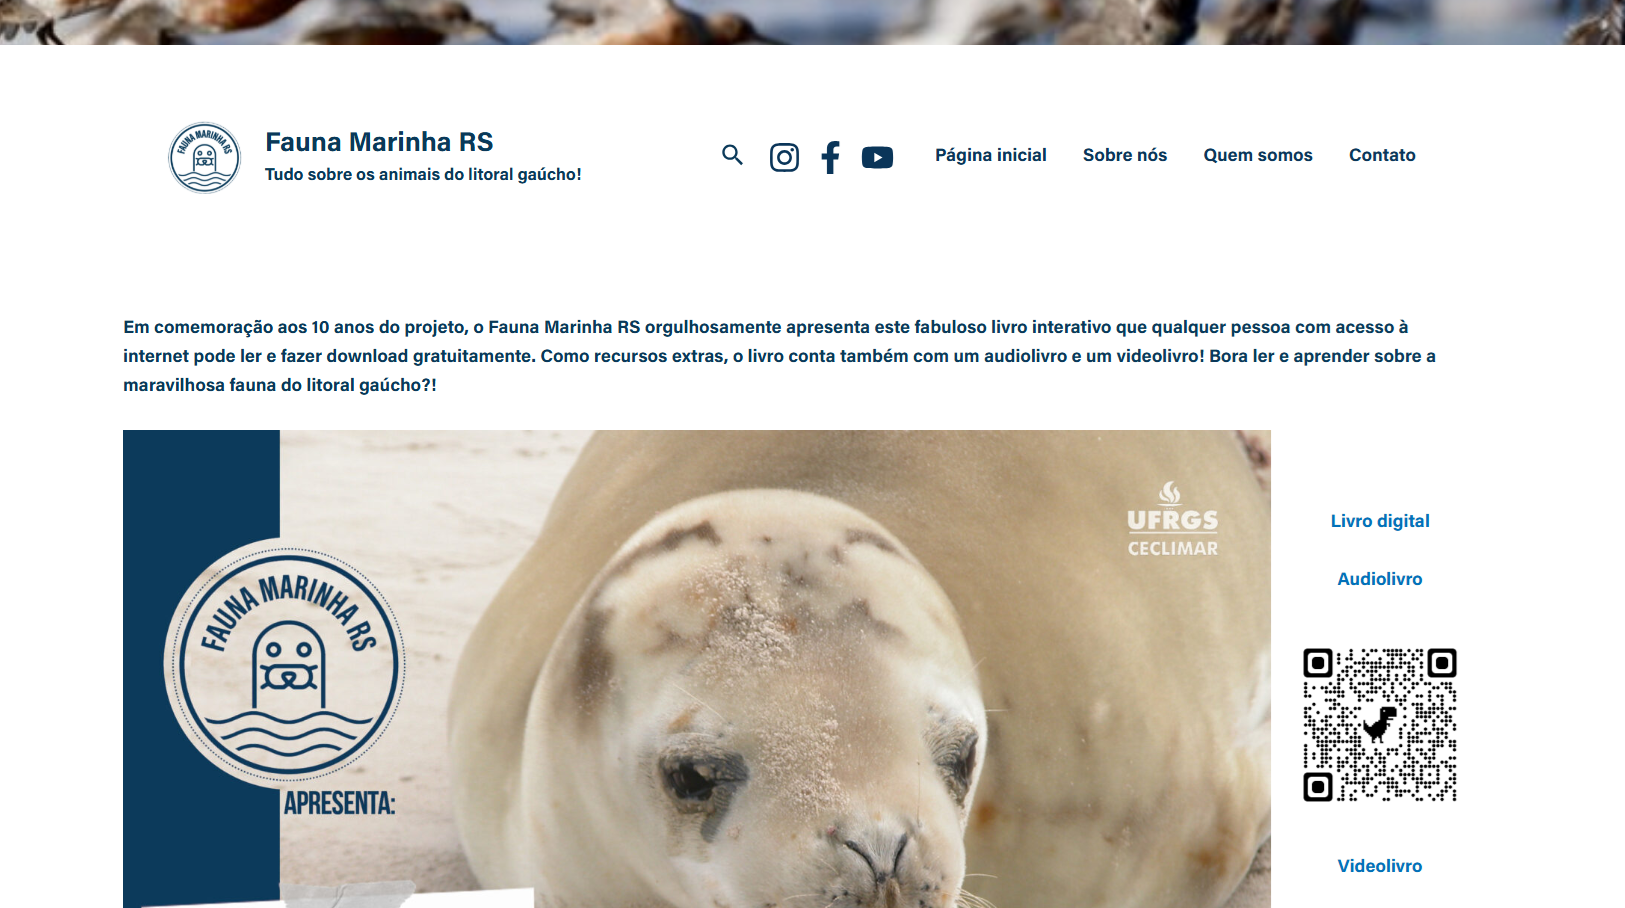
\includegraphics[width=1\textwidth]{imagens/sistemaWebFaunaMar.png}
    \caption{Identidade visual do sistema web do projeto Fauna Marinha RS.}
    \label{fig:identidade-visual-web}
\end{figure}
\legend{Fonte: \cite{faunamarinha2025}}

\begin{figure}[H]
    \centering
    
\includegraphics[height=0.5\textheight]{imagens/identidade-app.png}
    \caption{Identidade visual prototipada.}
    \label{fig:identidade-visual-mobile}
\end{figure}
\legend{Fonte: Autor}

\begin{figure}[H]
    \centering
    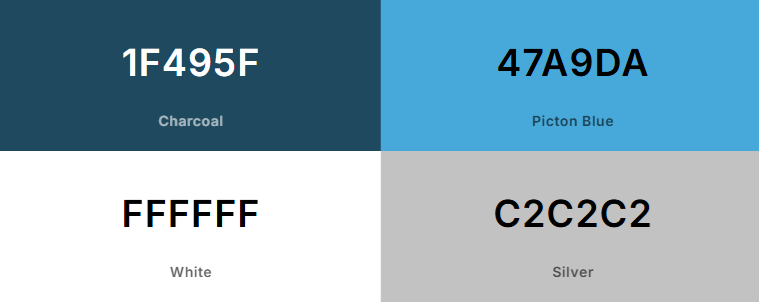
\includegraphics[width=1\textwidth]{imagens/paleta-cores.png}
    \caption{Paleta de cores utilizada.}
    \label{fig:paleta-cores}
\end{figure}
\legend{Fonte: Autor}

\subsection{Criação do Design das Telas}

Com base na identidade visual definida, foram elaborados os layouts das principais telas do 
aplicativo. Essa etapa concentrou-se na organização dos elementos de interface, na 
usabilidade e na experiência do usuário.

Inicialmente, foram criadas as telas de login (Figura~\ref{fig:prototipo-login}) e de 
registro de usuário (Figura~\ref{fig:prototipo-cadastro}).

\begin{figure}[H]
    \centering
    \begin{minipage}[b]{0.48\textwidth}
        \centering
        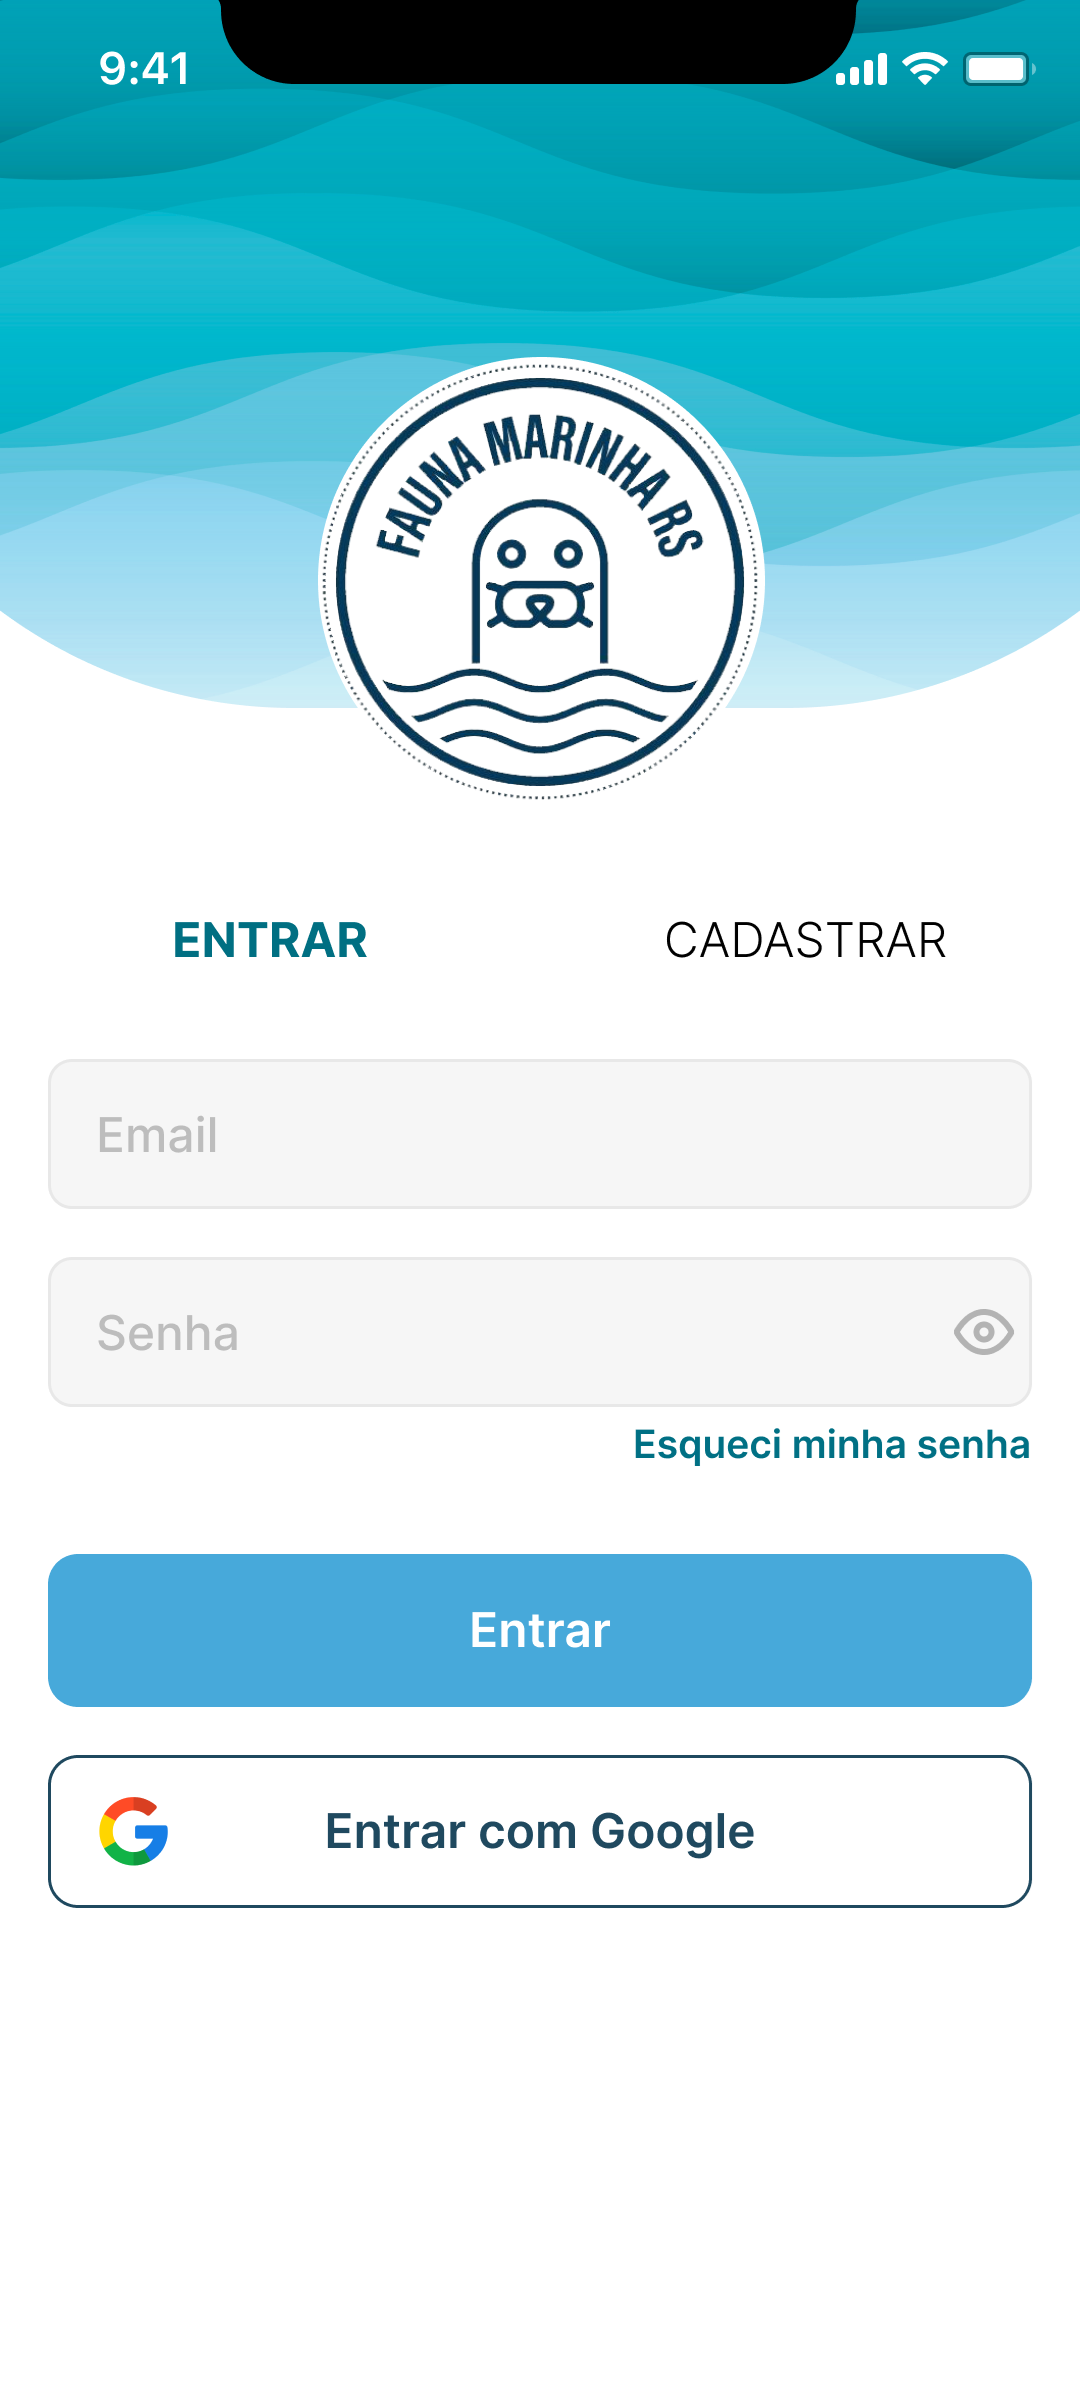
\includegraphics[height=0.6\textheight]{imagens/login-figma.png}
        \caption{Protótipo da tela de login do aplicativo.}
        \label{fig:prototipo-login}
    \end{minipage}
    \hfill
    \begin{minipage}[b]{0.48\textwidth}
        \centering
        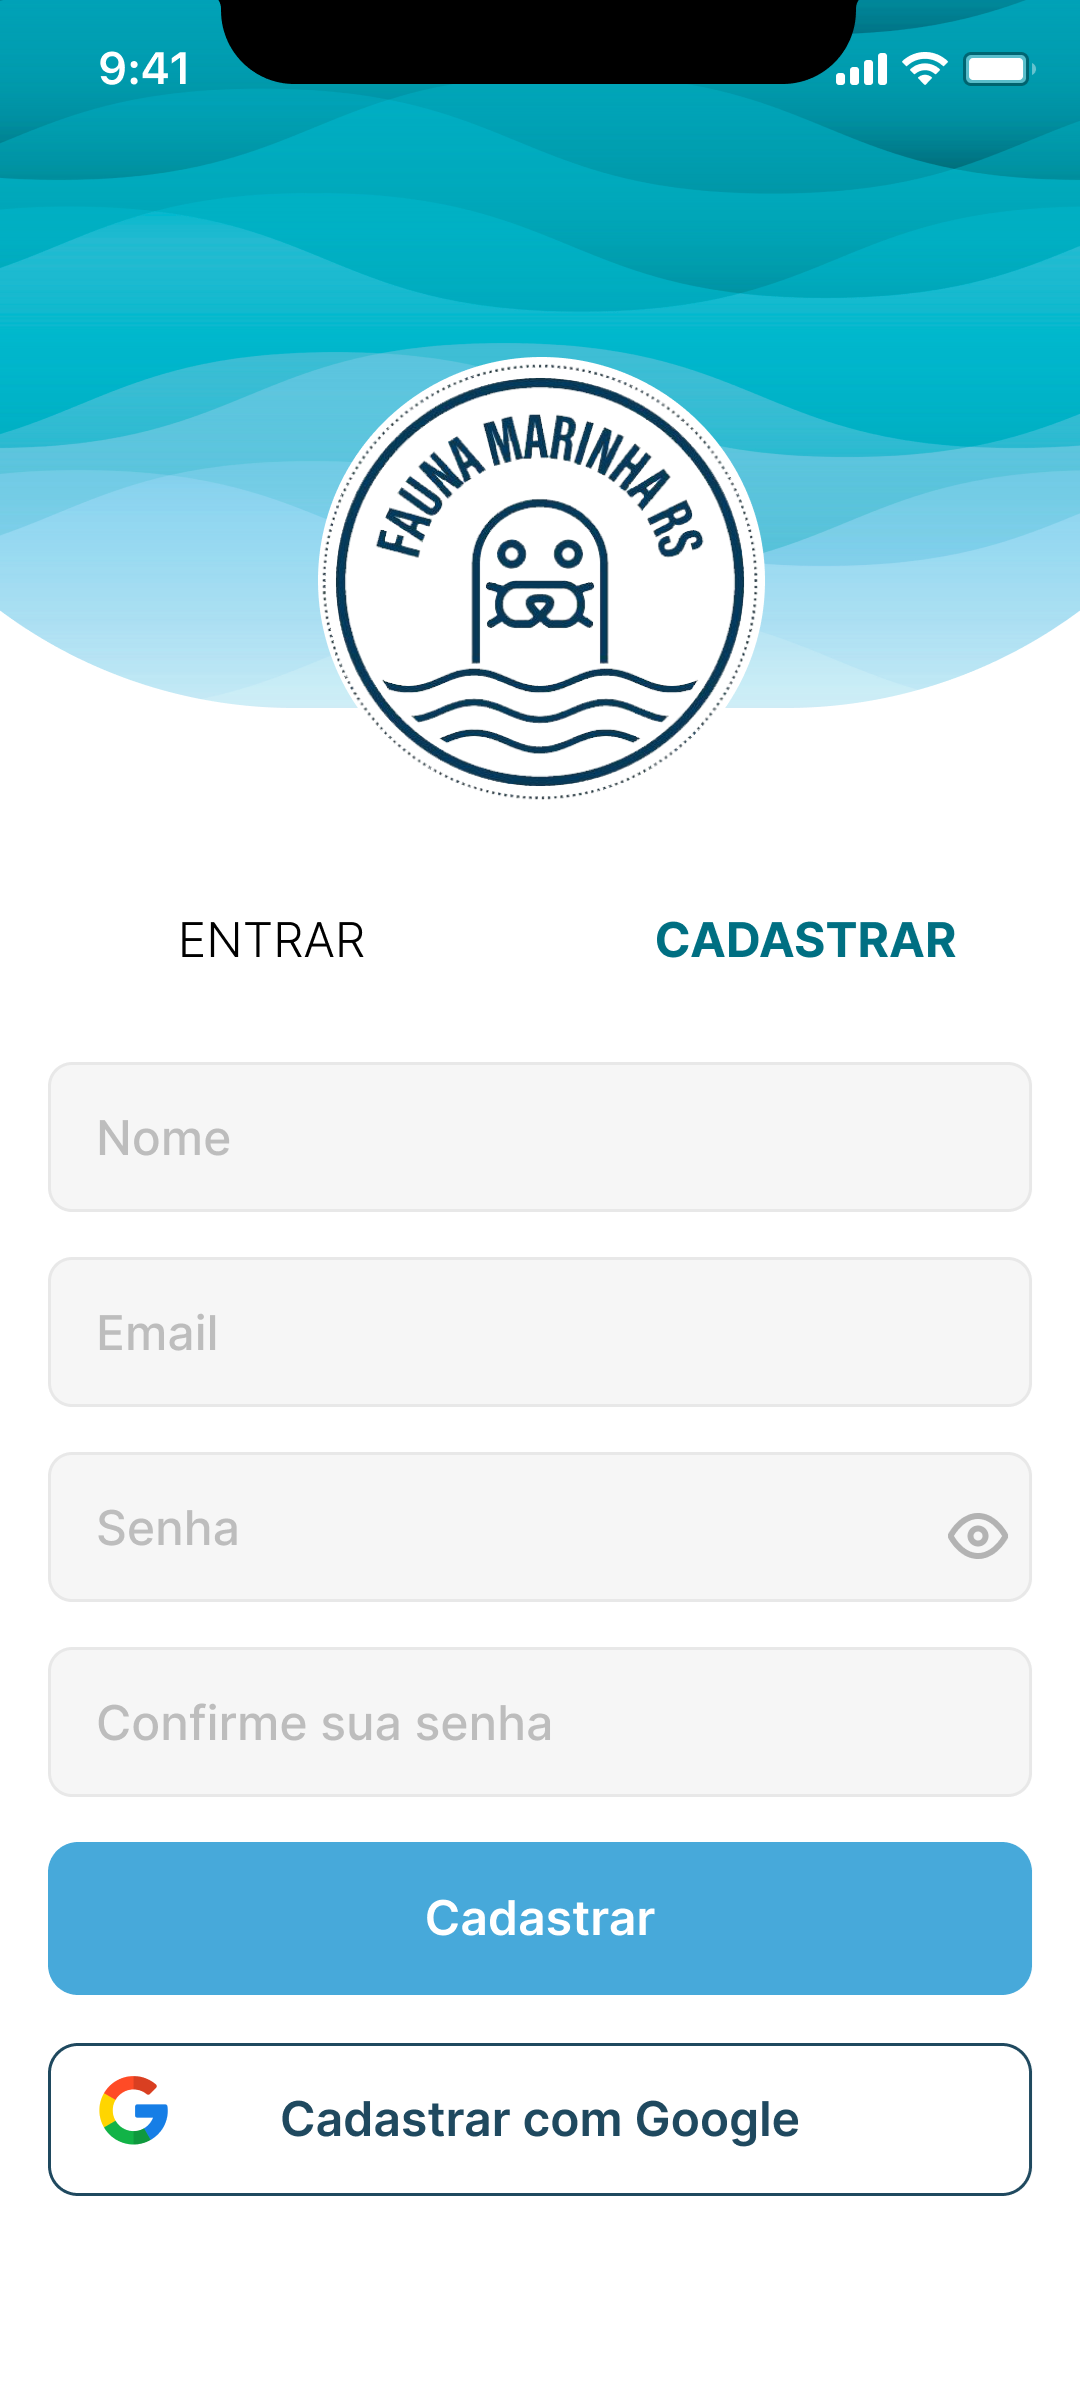
\includegraphics[height=0.6\textheight]{imagens/cadastro-figma.png}
        \caption{Protótipo da tela de cadastro do aplicativo.}
        \label{fig:prototipo-cadastro}
    \end{minipage}
\end{figure}
\legend{Fonte: Autor}

Em seguida, foi criada a tela inicial (Figura~\ref{fig:prototipo-home}), com duas 
variações: uma para usuários comuns e outra para pesquisadores. O layout foi pensado 
para facilitar o acesso às funcionalidades, com botões de acesso rápido e 
barra de navegação fixa na parte inferior da tela. A versão para pesquisadores apresenta os mesmos botões,
com a adição das funcionalidades exclusivas, avaliação de registros e acesso ao painel geral.

\begin{figure}[H]
    \centering
    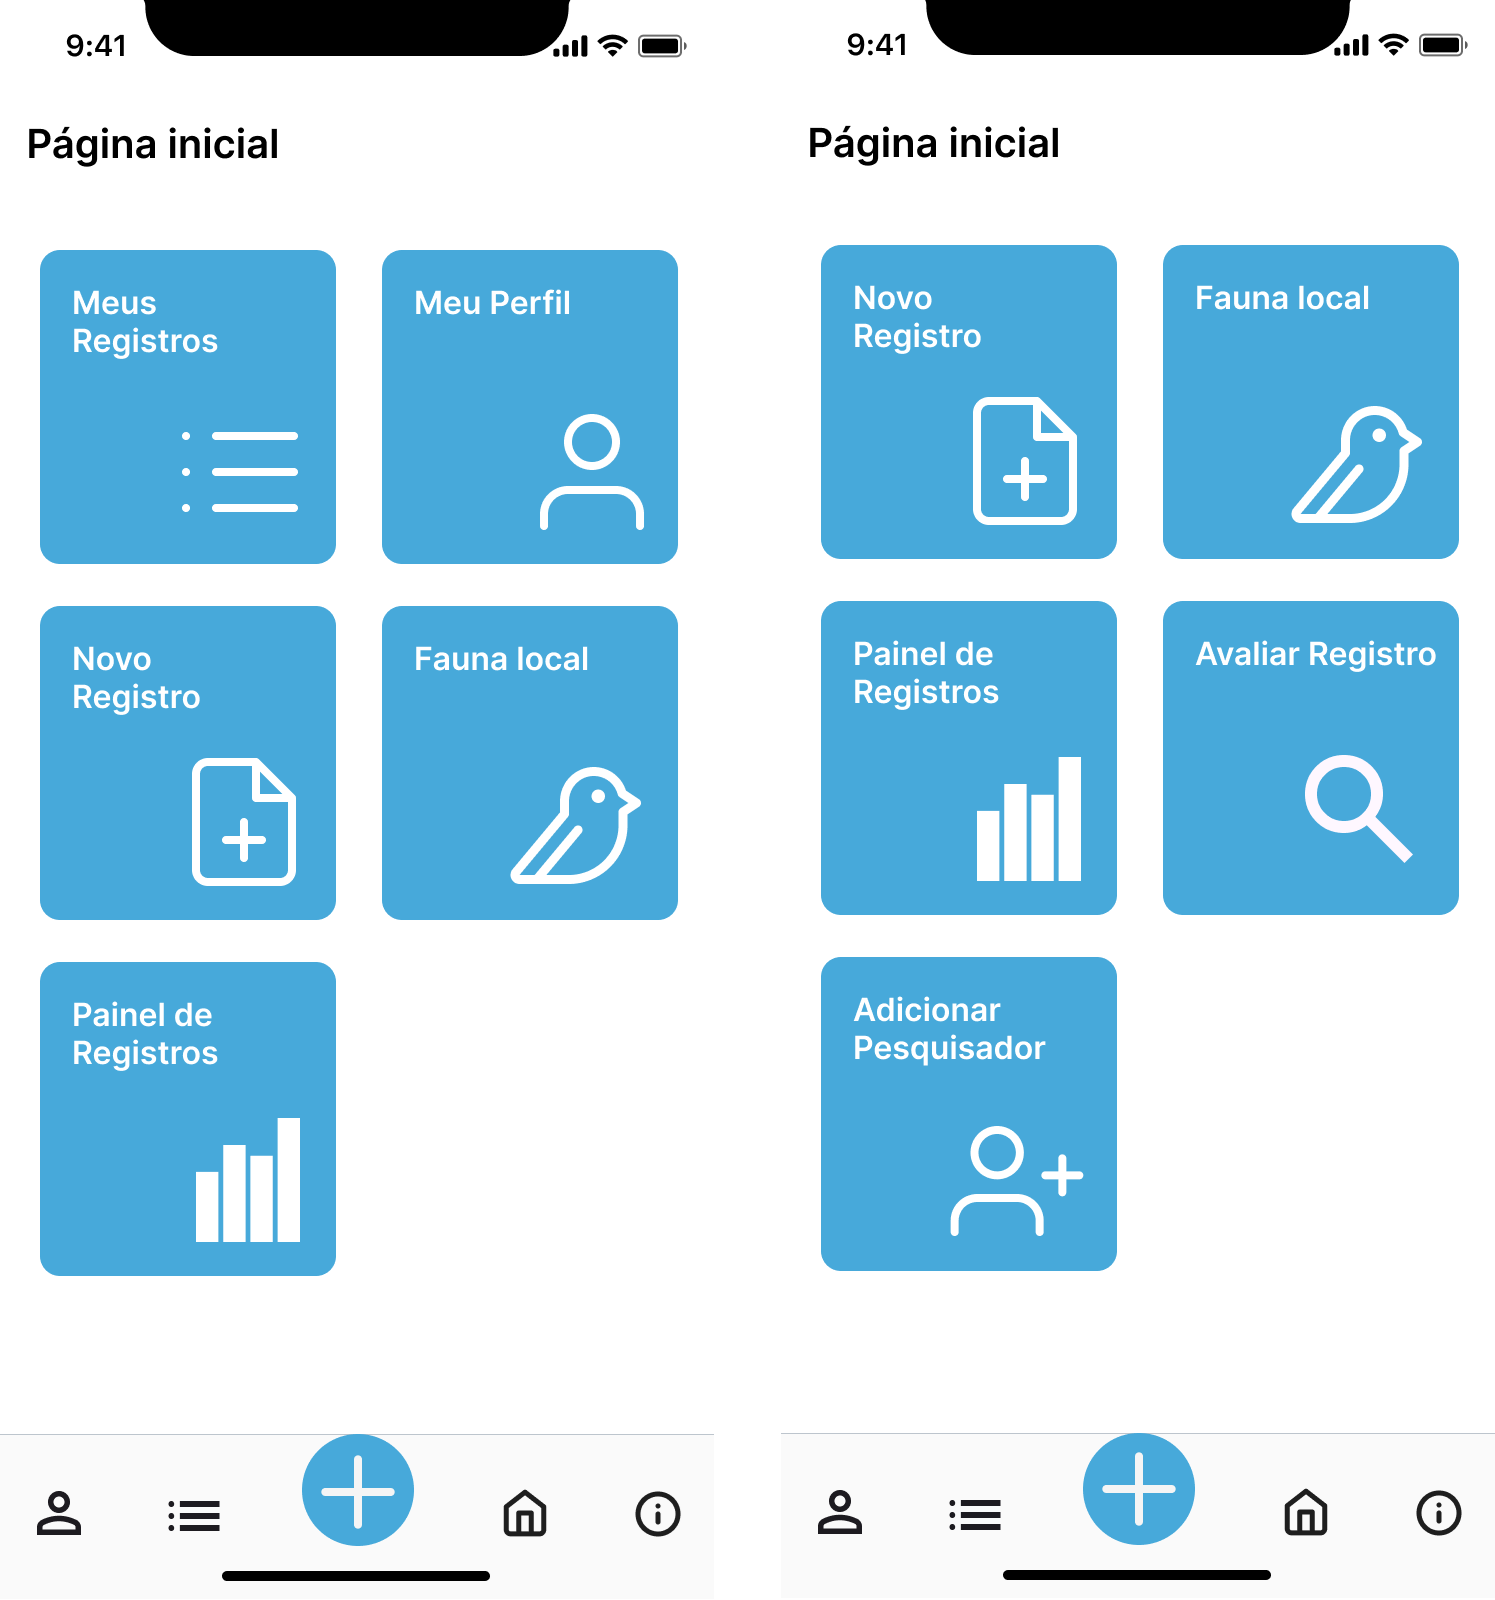
\includegraphics[height=0.6\textheight]{imagens/menu-pesquisador-figma.png}
    \caption{Protótipo da tela inicial: usuário comum (esquerda) e pesquisador (direita).}
    \label{fig:prototipo-home}
\end{figure}
\legend{Fonte: Autor}

A tela "Meus Registros" (Figura~\ref{fig:prototipo-meus-registros}) permite ao usuário 
visualizar todos os registros já enviados, com filtros por status (enviado e validado). 
Também foi projetado um estado com \textit{bottomsheet} acionado a partir do botão de adicionar 
registro ("+") na barra de navegação. Esse botão está disponível em qualquer tela, permitindo 
adicionar registros rapidamente.

\begin{figure}[H]
    \centering
    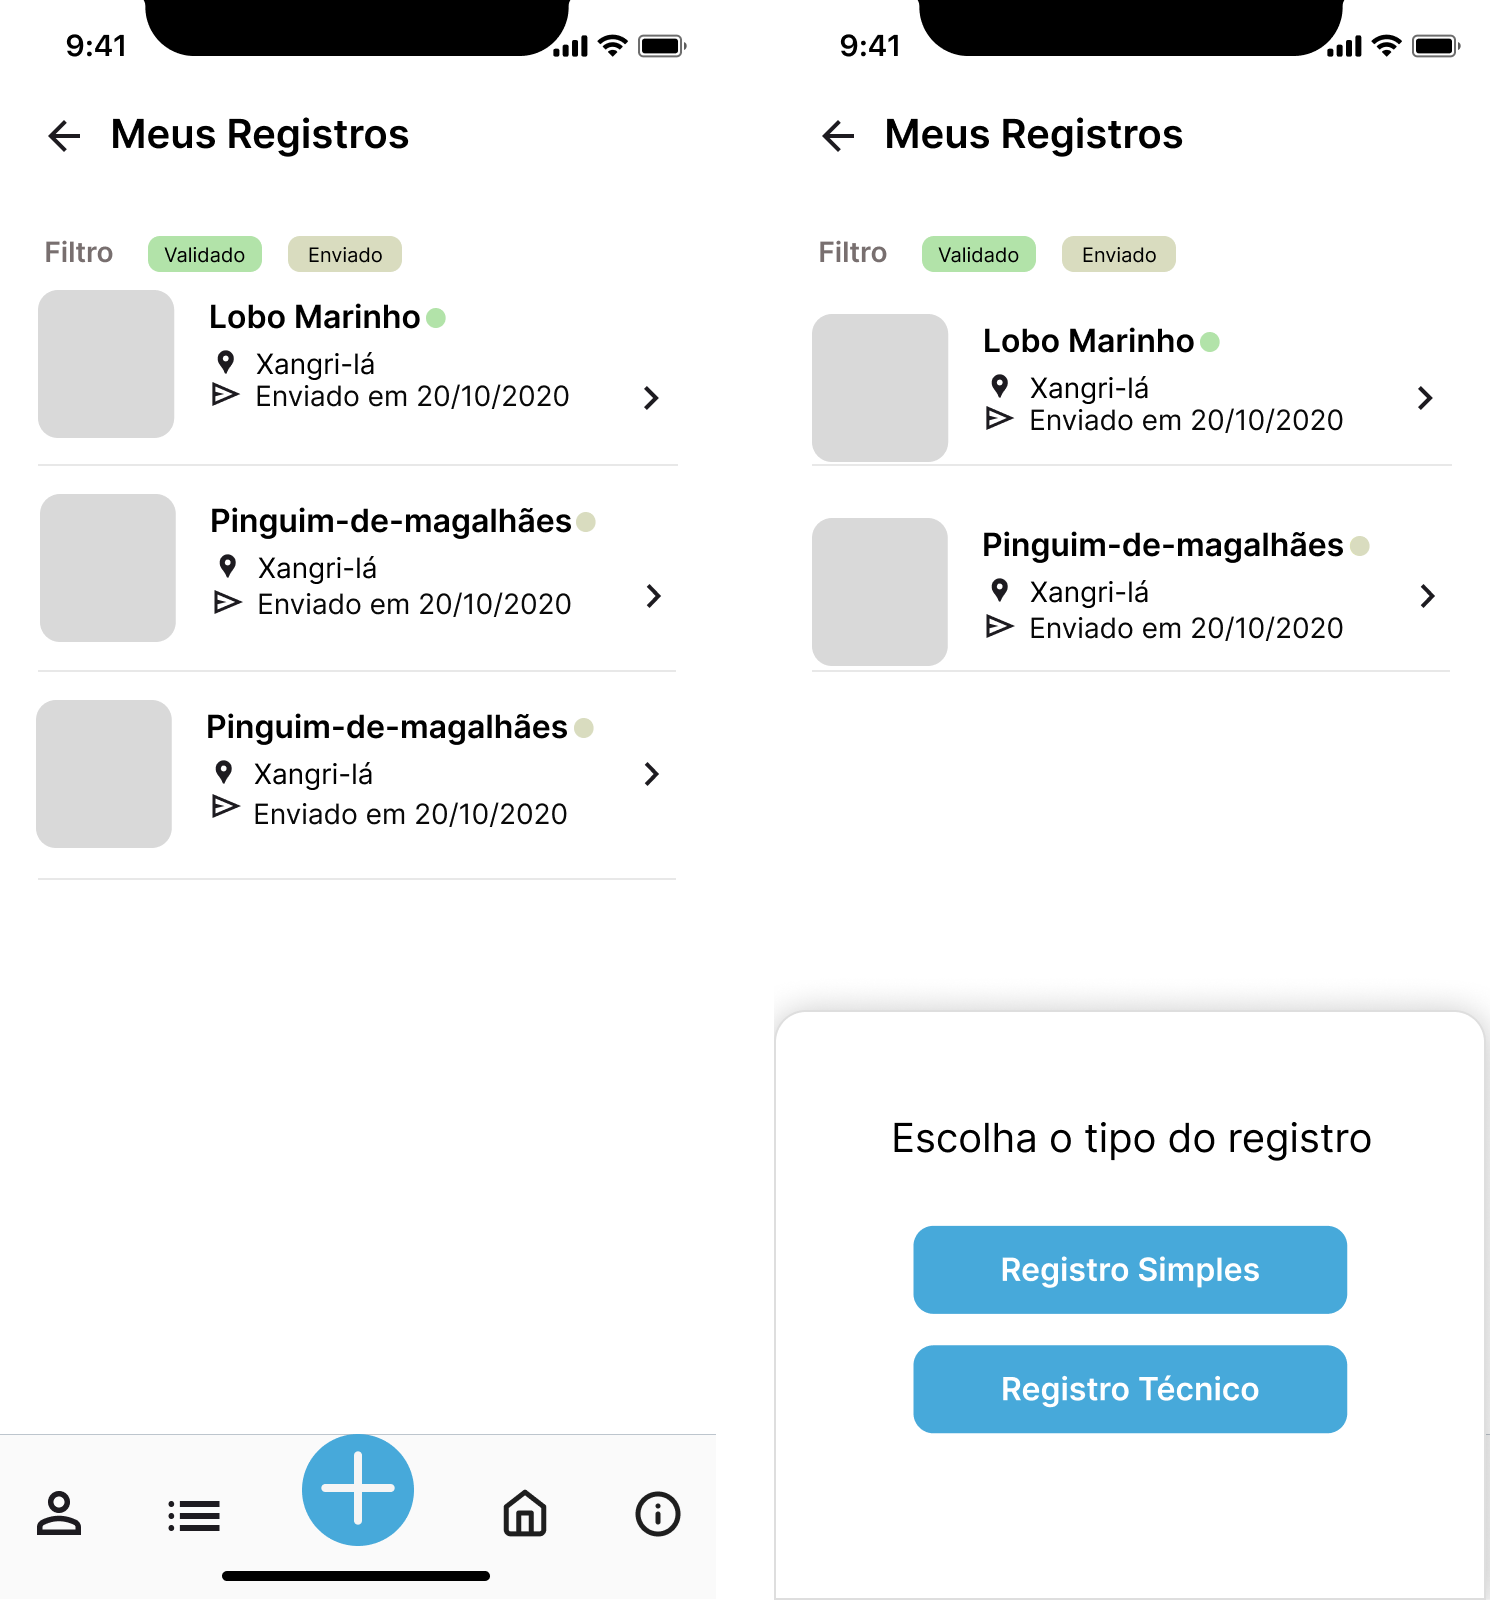
\includegraphics[height=0.6\textheight]{imagens/meus-registros-figma.png}
    \caption{Protótipo das telas de "Meus Registros" com estado ativo de adição de registro (direita).}
    \label{fig:prototipo-meus-registros}
\end{figure}
\legend{Fonte: Autor}

Dois tipos de formulários de registro foram projetados: um simples
 (Figura~\ref{fig:prototipo-registro-simples}), voltado a usuários leigos e envios rápidos, e 
 outro técnico (Figura~\ref{fig:prototipo-registro-tecnico}), com campos adicionais 
 para coleta de dados mais detalhados. Ambos possuem validações, campos obrigatórios e 
 opcionais, e suporte ao envio de imagens com orientações apresentadas em \textit{bottomsheet}.

Os campos específicos de classe, ordem, família e gênero foram projetados para serem um dropdown,
que apresentará as opções disponíveis para o usuário selecionar.

\begin{figure}[H]
    \centering
    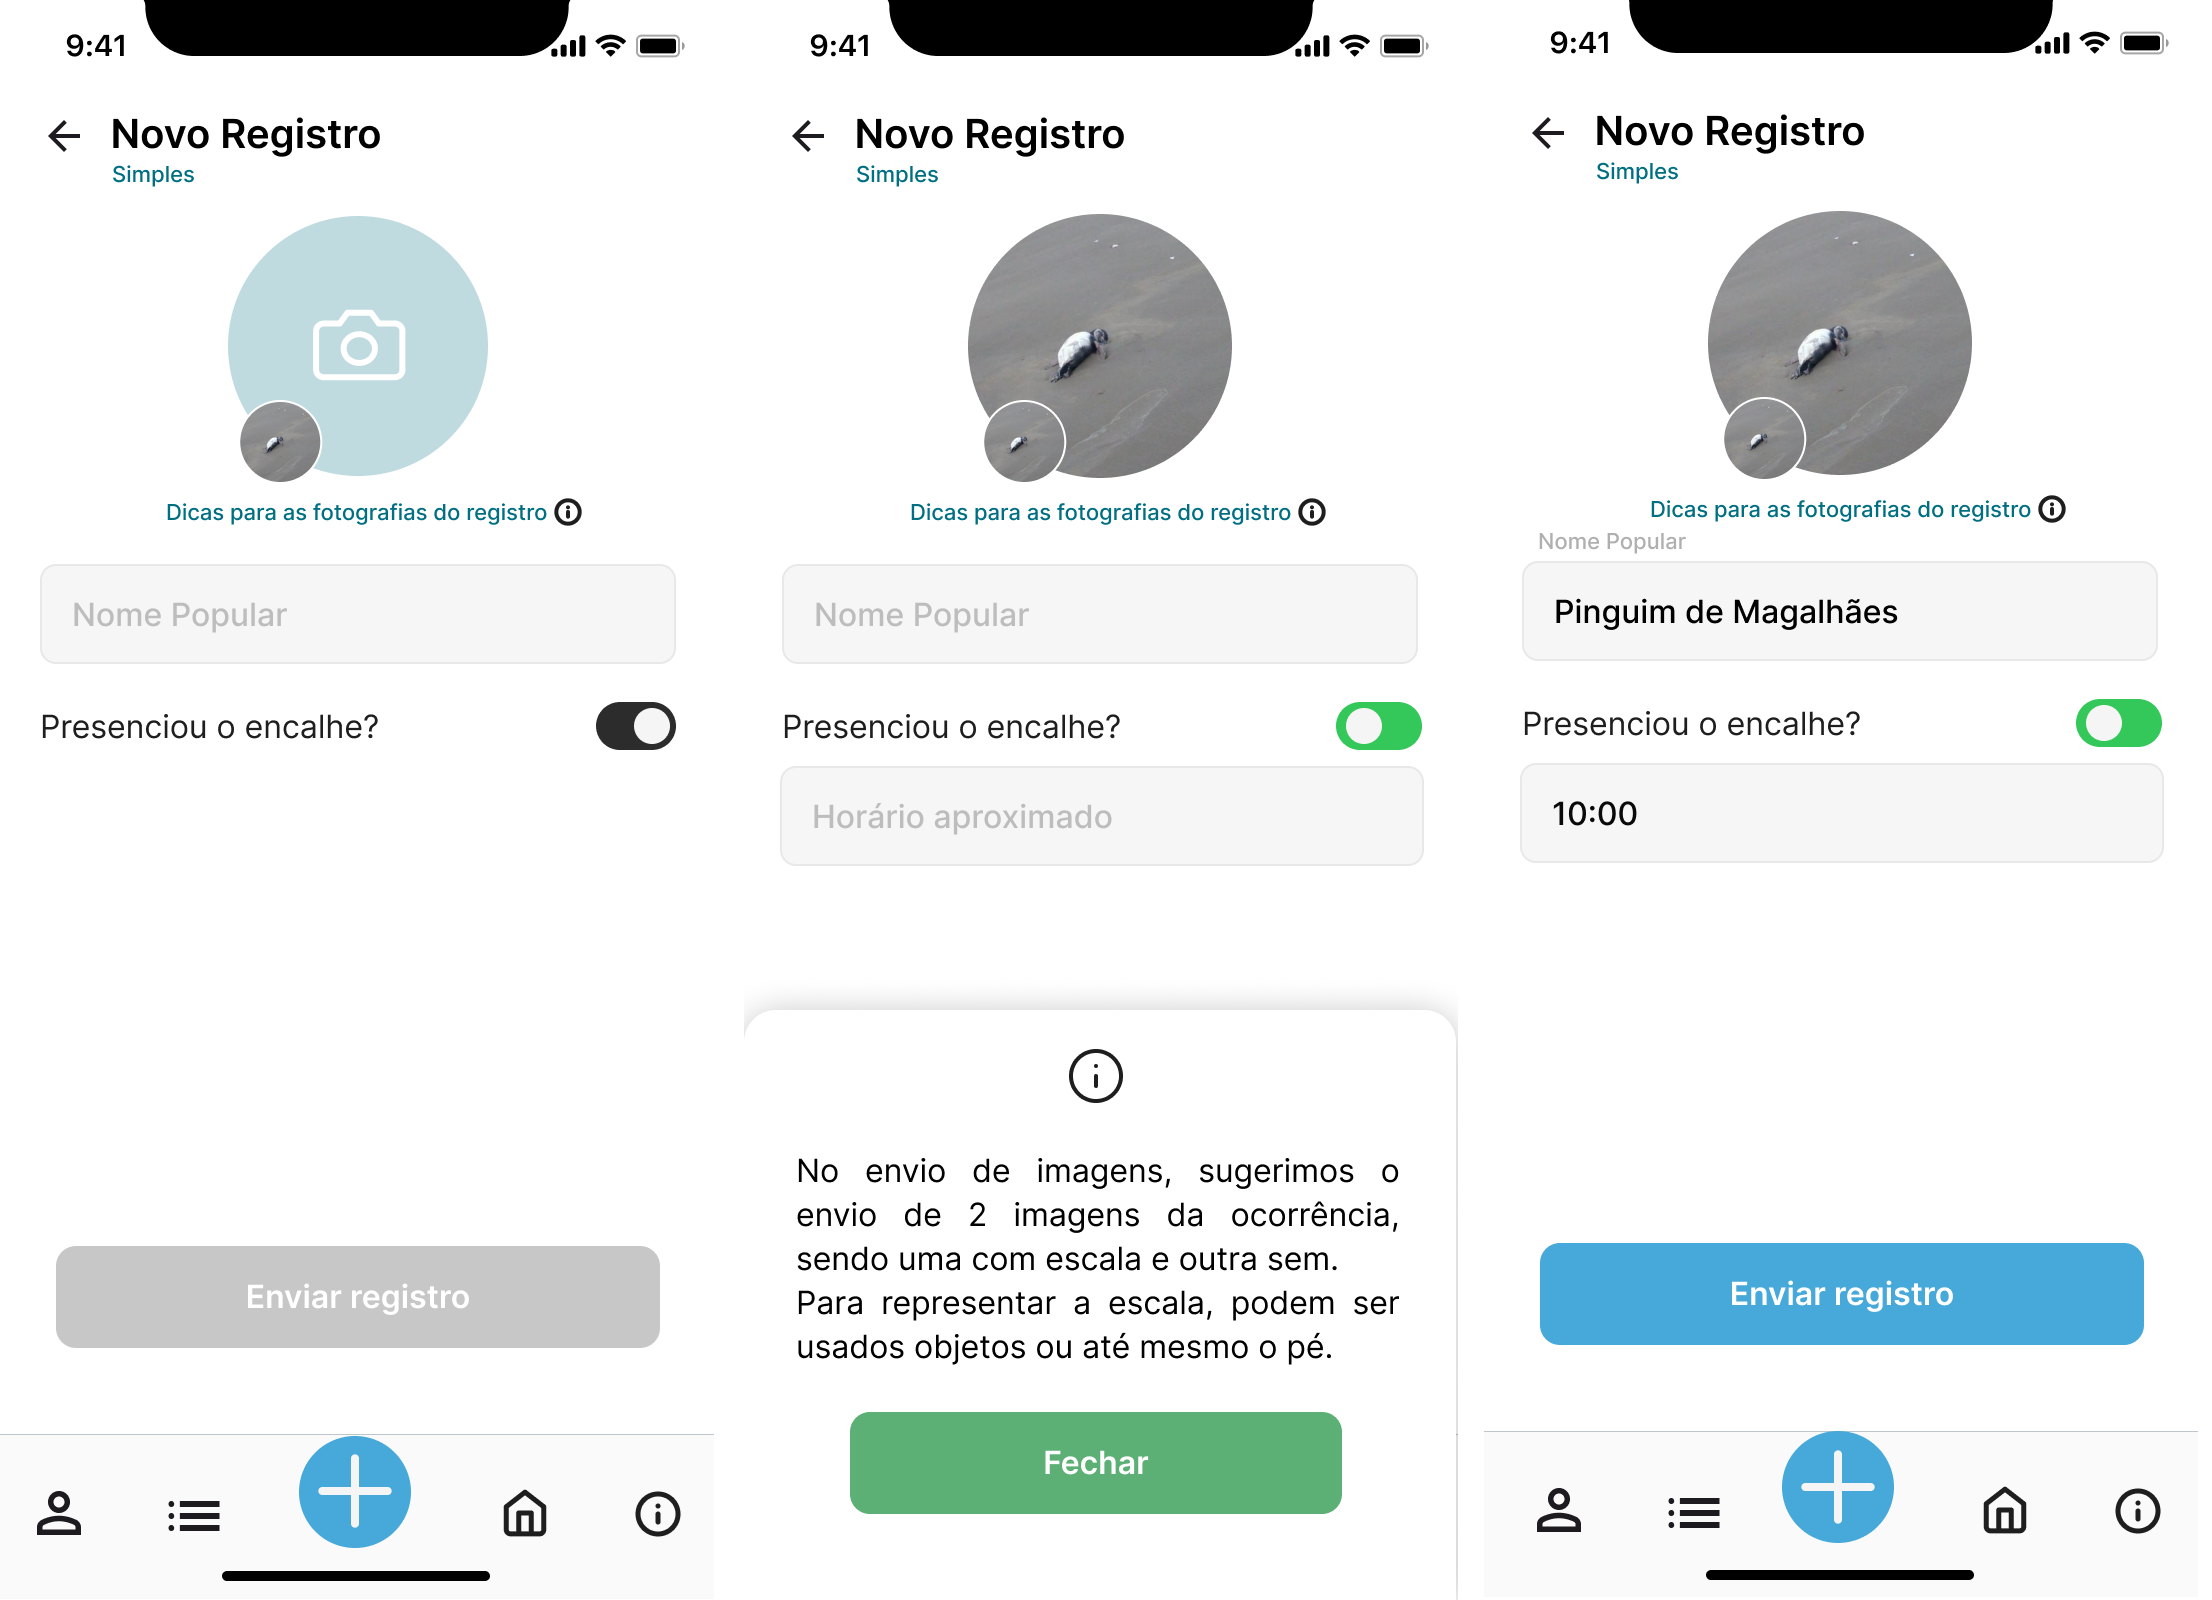
\includegraphics[height=0.55\textheight, width=\textwidth]{imagens/registro-simples-figma.png}
    \caption{Protótipo do formulário de registro simples. Centro: \textit{bottomsheet} informativa; direita: campo 
    adicional ativado.}
    \label{fig:prototipo-registro-simples}
\end{figure}
\legend{Fonte: Autor}

\begin{figure}[H]
    \centering
    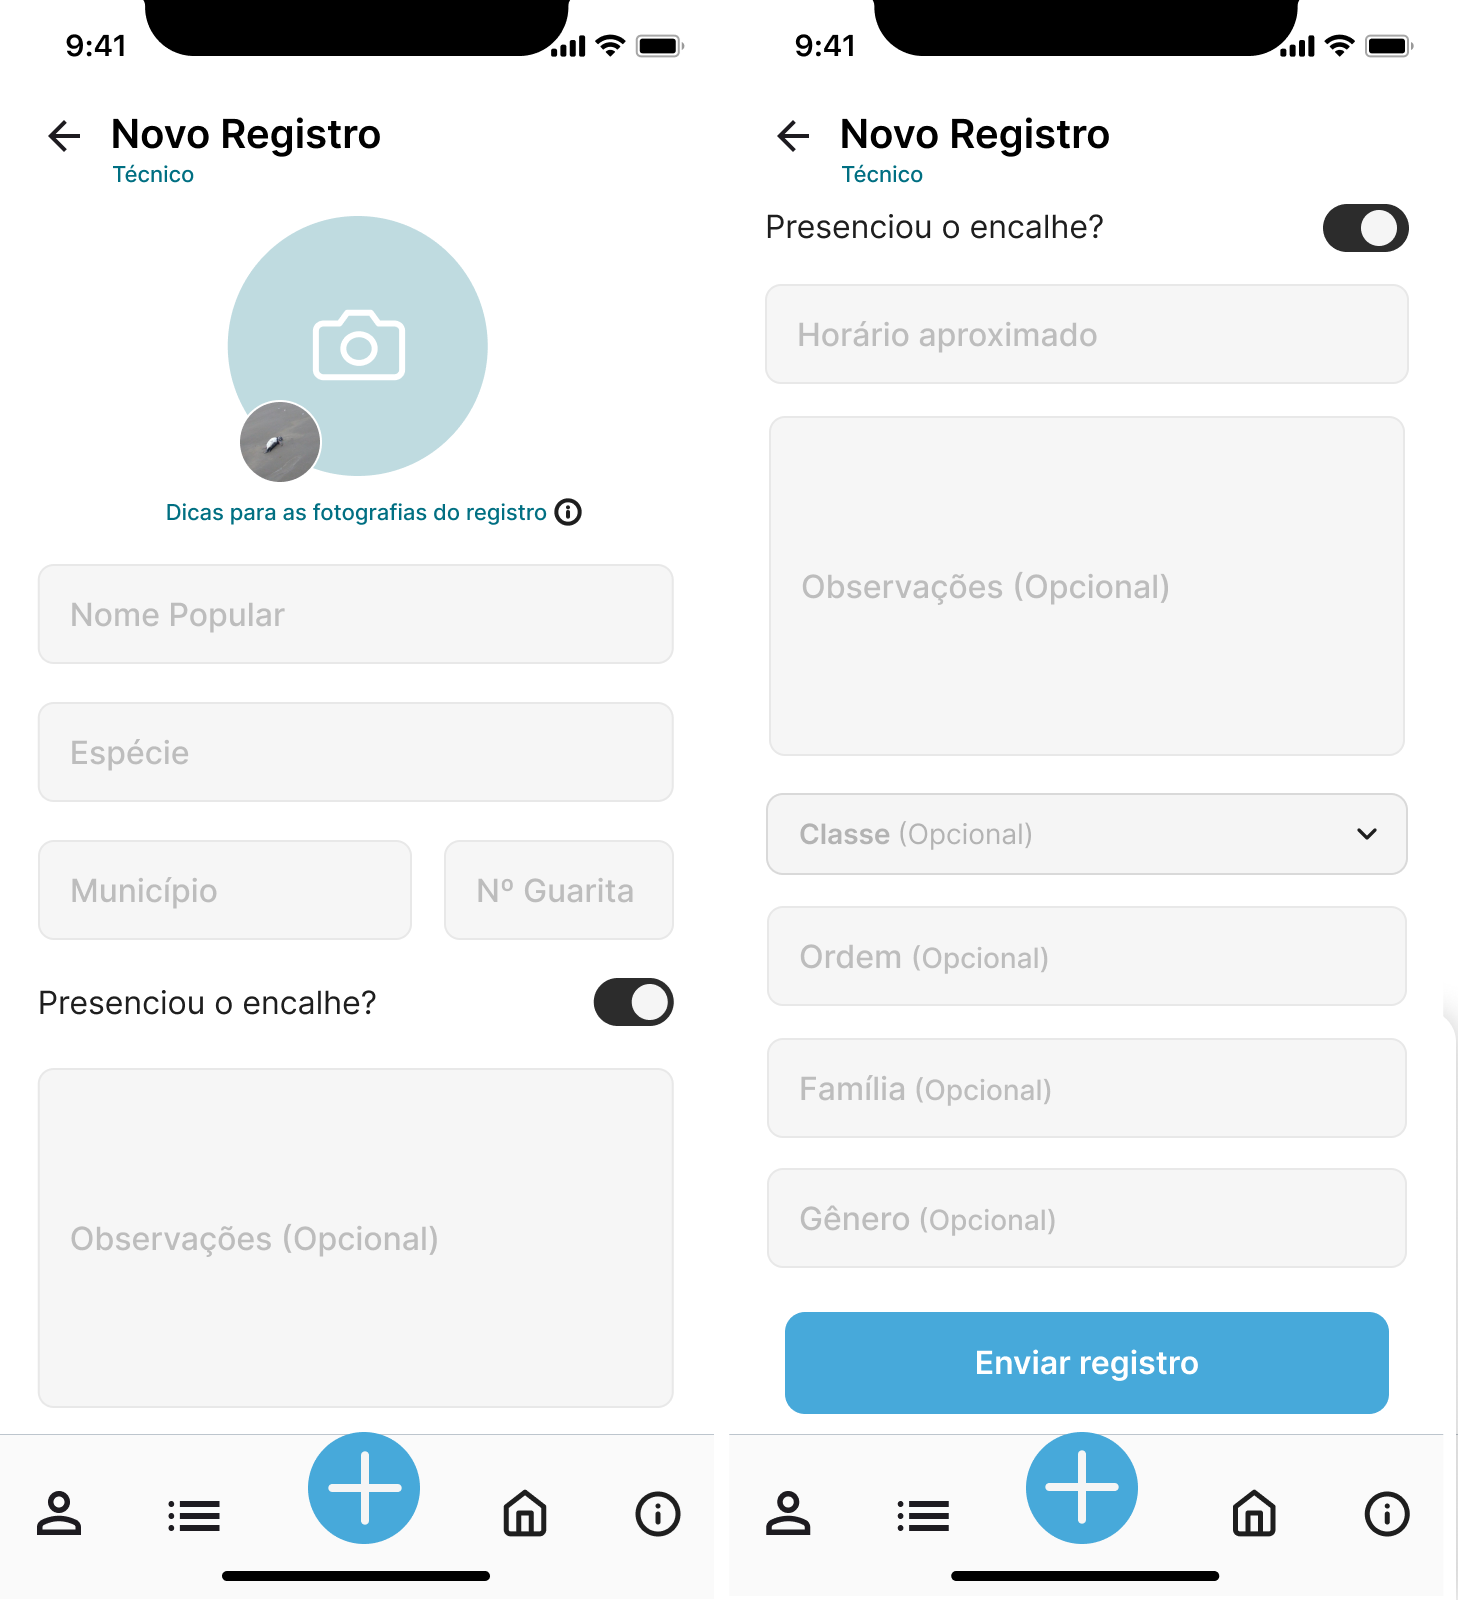
\includegraphics[height=0.6\textheight]{imagens/registro-tecnico-figma.png}
    \caption{Protótipo do formulário de registro técnico com campos taxonômicos e detalhamento avançado.}
    \label{fig:prototipo-registro-tecnico}
\end{figure}
\legend{Fonte: Autor}

A tela de "Registros Pendentes" (Figura~\ref{fig:prototipo-registros-pendentes}) foi projetada 
para uso exclusivo de pesquisadores, permitindo acesso aos registros ainda não avaliados enviados 
por todos os usuários.

\begin{figure}[H]
    \centering
    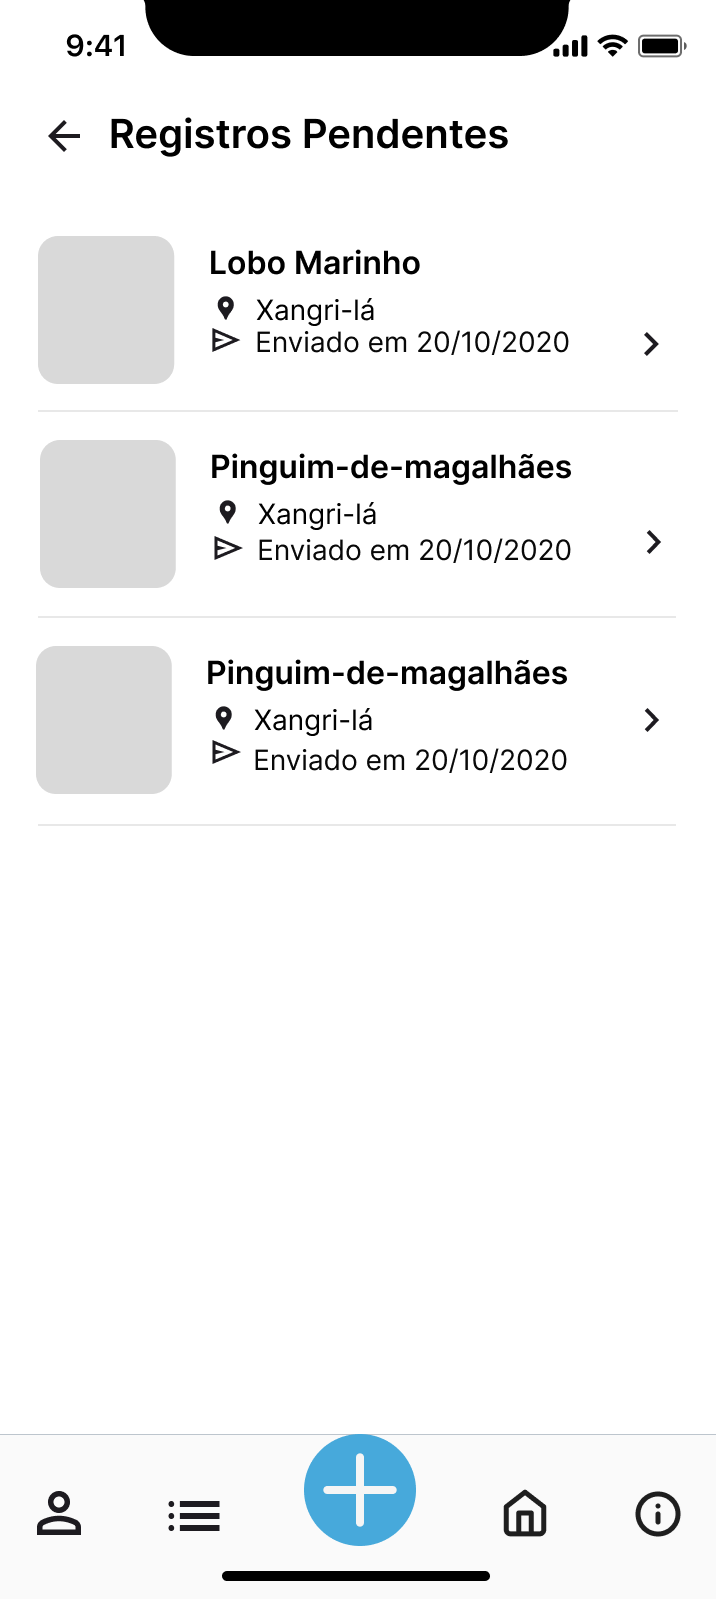
\includegraphics[height=0.6\textheight]{imagens/registro-pendente-figma.png}
    \caption{Protótipo da tela de registros pendentes, acessível apenas a pesquisadores.}
    \label{fig:prototipo-registros-pendentes}
\end{figure}
\legend{Fonte: Autor}

A tela de "Analisar Registro" (Figura~\ref{fig:prototipo-avaliar-registro}) foi projetada para 
permitir que o pesquisador visualize os dados enviados em cada registro 
com a possibilidade de editar os dados, adicionar comentários e enviar uma atualização o registro.
Se fez importante adicionar um estado para esta tela, onde o pesquisador consiga selecionar a imagem
para uma visualização em tela cheia, facilitando a análise do registro.

\begin{figure}[H]
    \centering
    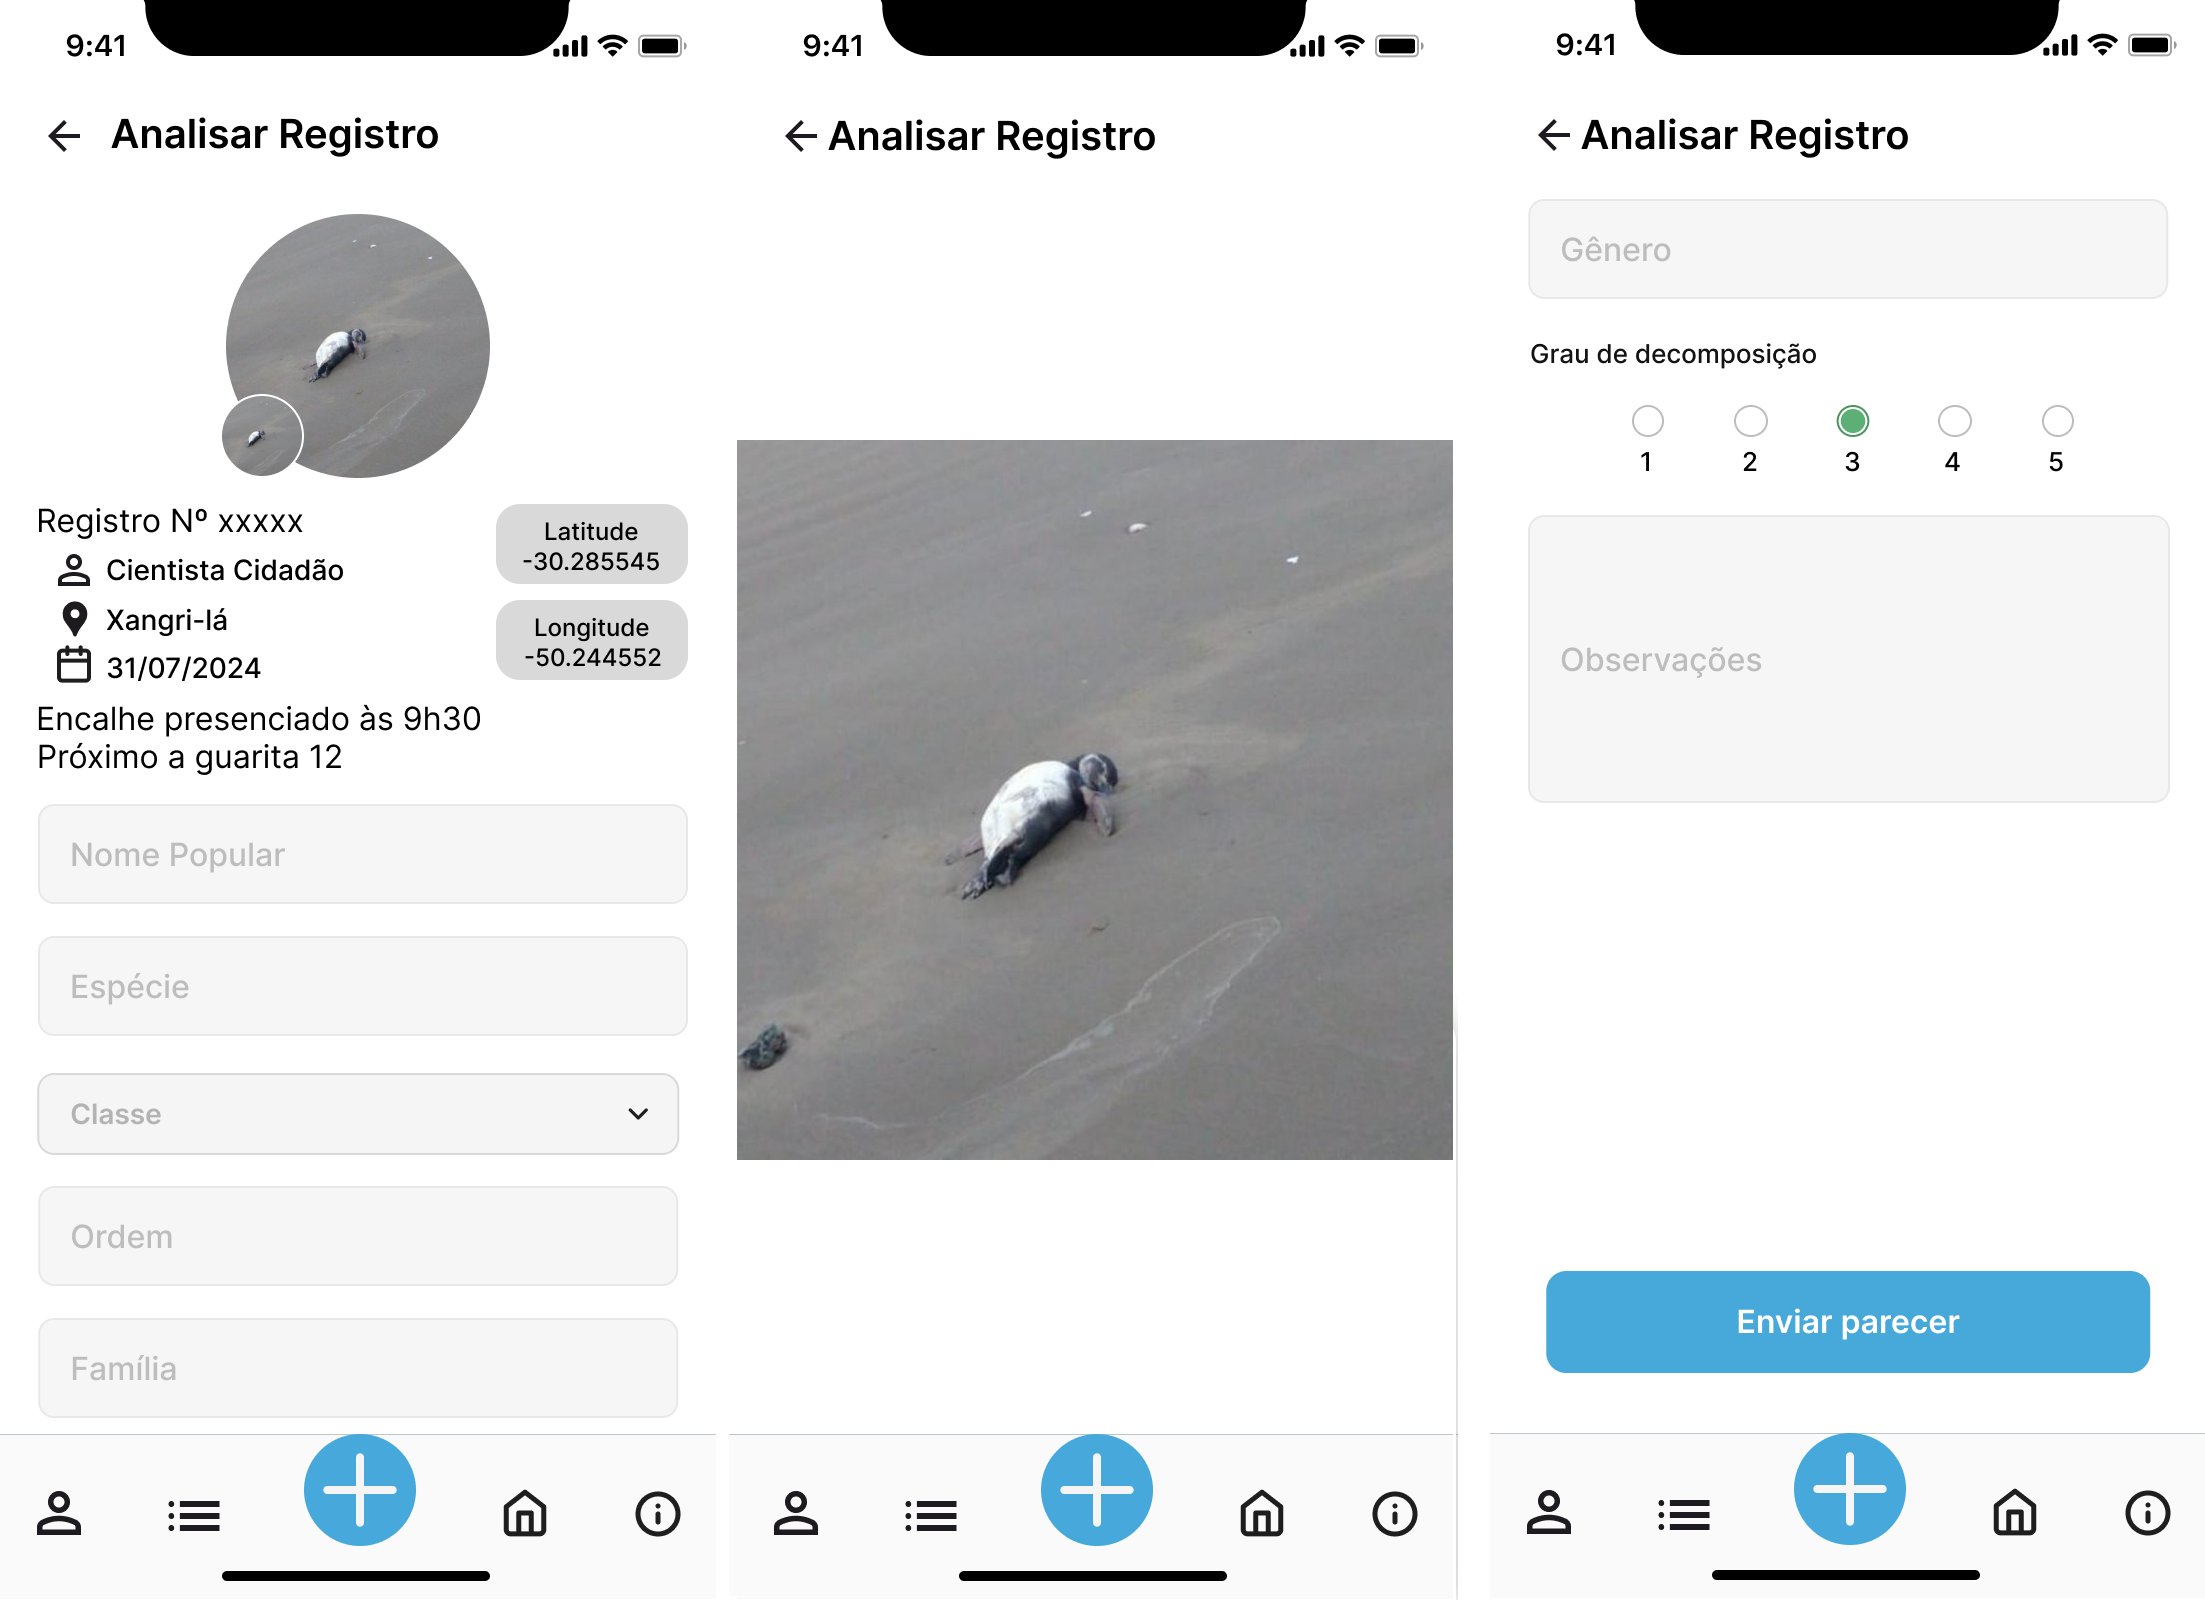
\includegraphics[height=0.55\textheight, width=\textwidth]{imagens/avaliar-registro-figma.png}
    \caption{Protótipo da tela de análise de registro. Ao centro, visualização ampliada da imagem.}
    \label{fig:prototipo-avaliar-registro}
\end{figure}
\legend{Fonte: Autor}

A tela de "Visualizar Registro" foi projetada para permitir que o usuário visualize os dados
enviados e validados. Para os dados já foram validados 
(Figura~\ref{fig:prototipo-ver-registro-validado}), o registro apresentará dados extras 
sobre aquele registro, como grau de decomposição, parecer do profissional e taxonomia avaliada.
Já para os dados que ainda não foram validados (Figura~\ref{fig:prototipo-ver-registro-enviado}), 
o usuário verá apenas as informações que ele mesmo enviou.

\begin{figure}[H]
    \centering
    \begin{minipage}[b]{0.48\textwidth}
        \centering
        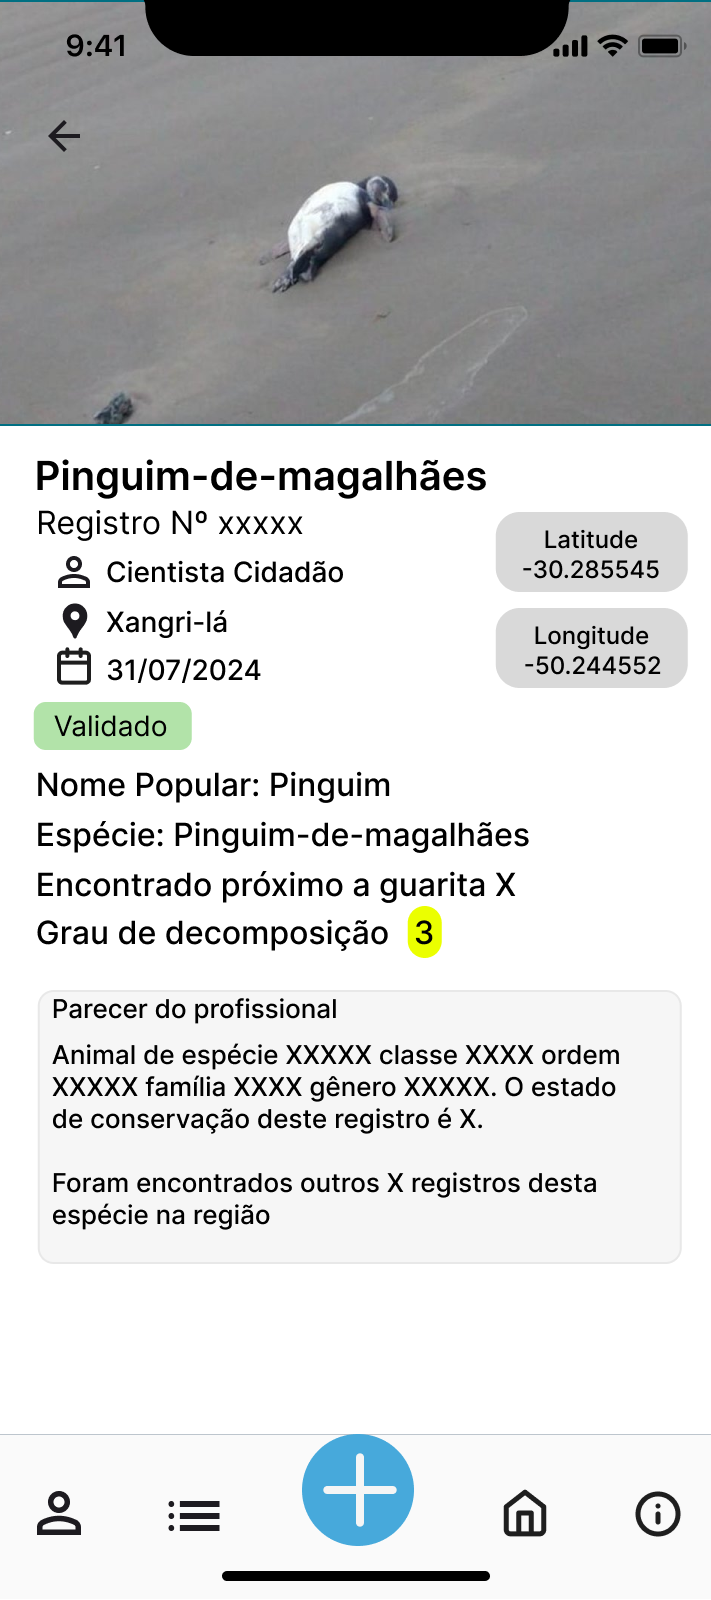
\includegraphics[height=0.6\textheight]{imagens/ver-registro-figma.png}
        \caption{Protótipo da visualização de registro validado.}
        \label{fig:prototipo-ver-registro-validado}
    \end{minipage}
    \hfill
    \begin{minipage}[b]{0.48\textwidth}
        \centering
        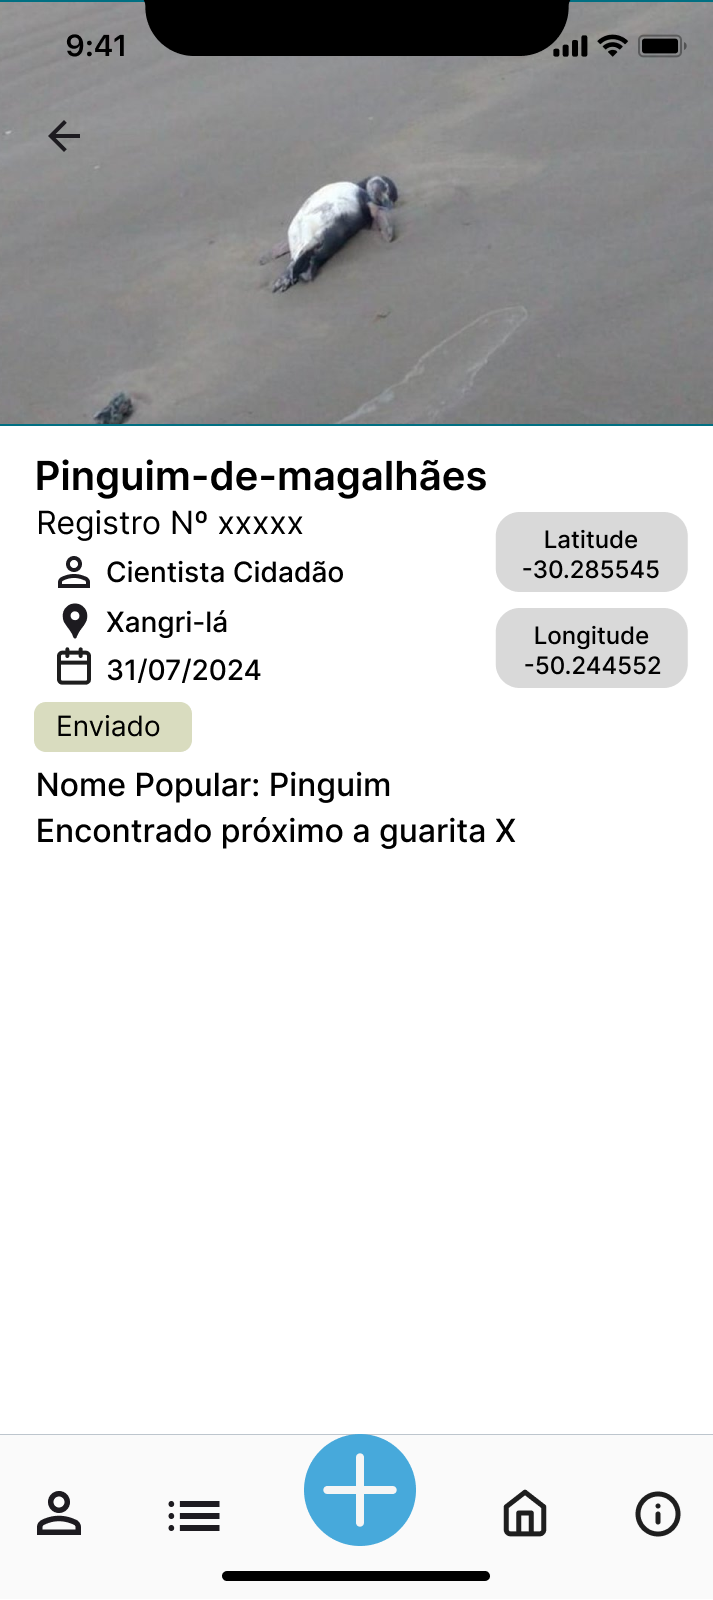
\includegraphics[height=0.6\textheight]{imagens/ve-registro-enviado-figma.png}
        \caption{Protótipo da visualização de registro enviado, ainda não avaliado.}
        \label{fig:prototipo-ver-registro-enviado}
    \end{minipage}
\end{figure}
\legend{Fonte: Autor}

A tela de perfil do usuário (Figura~\ref{fig:prototipo-perfil}) apresenta dados básicos, 
quantidade de registros enviados, últimos registros e conquistas. As conquistas são exibidas 
em formato de medalhas organizadas em uma grade com três colunas.

\begin{figure}[H]
    \centering
    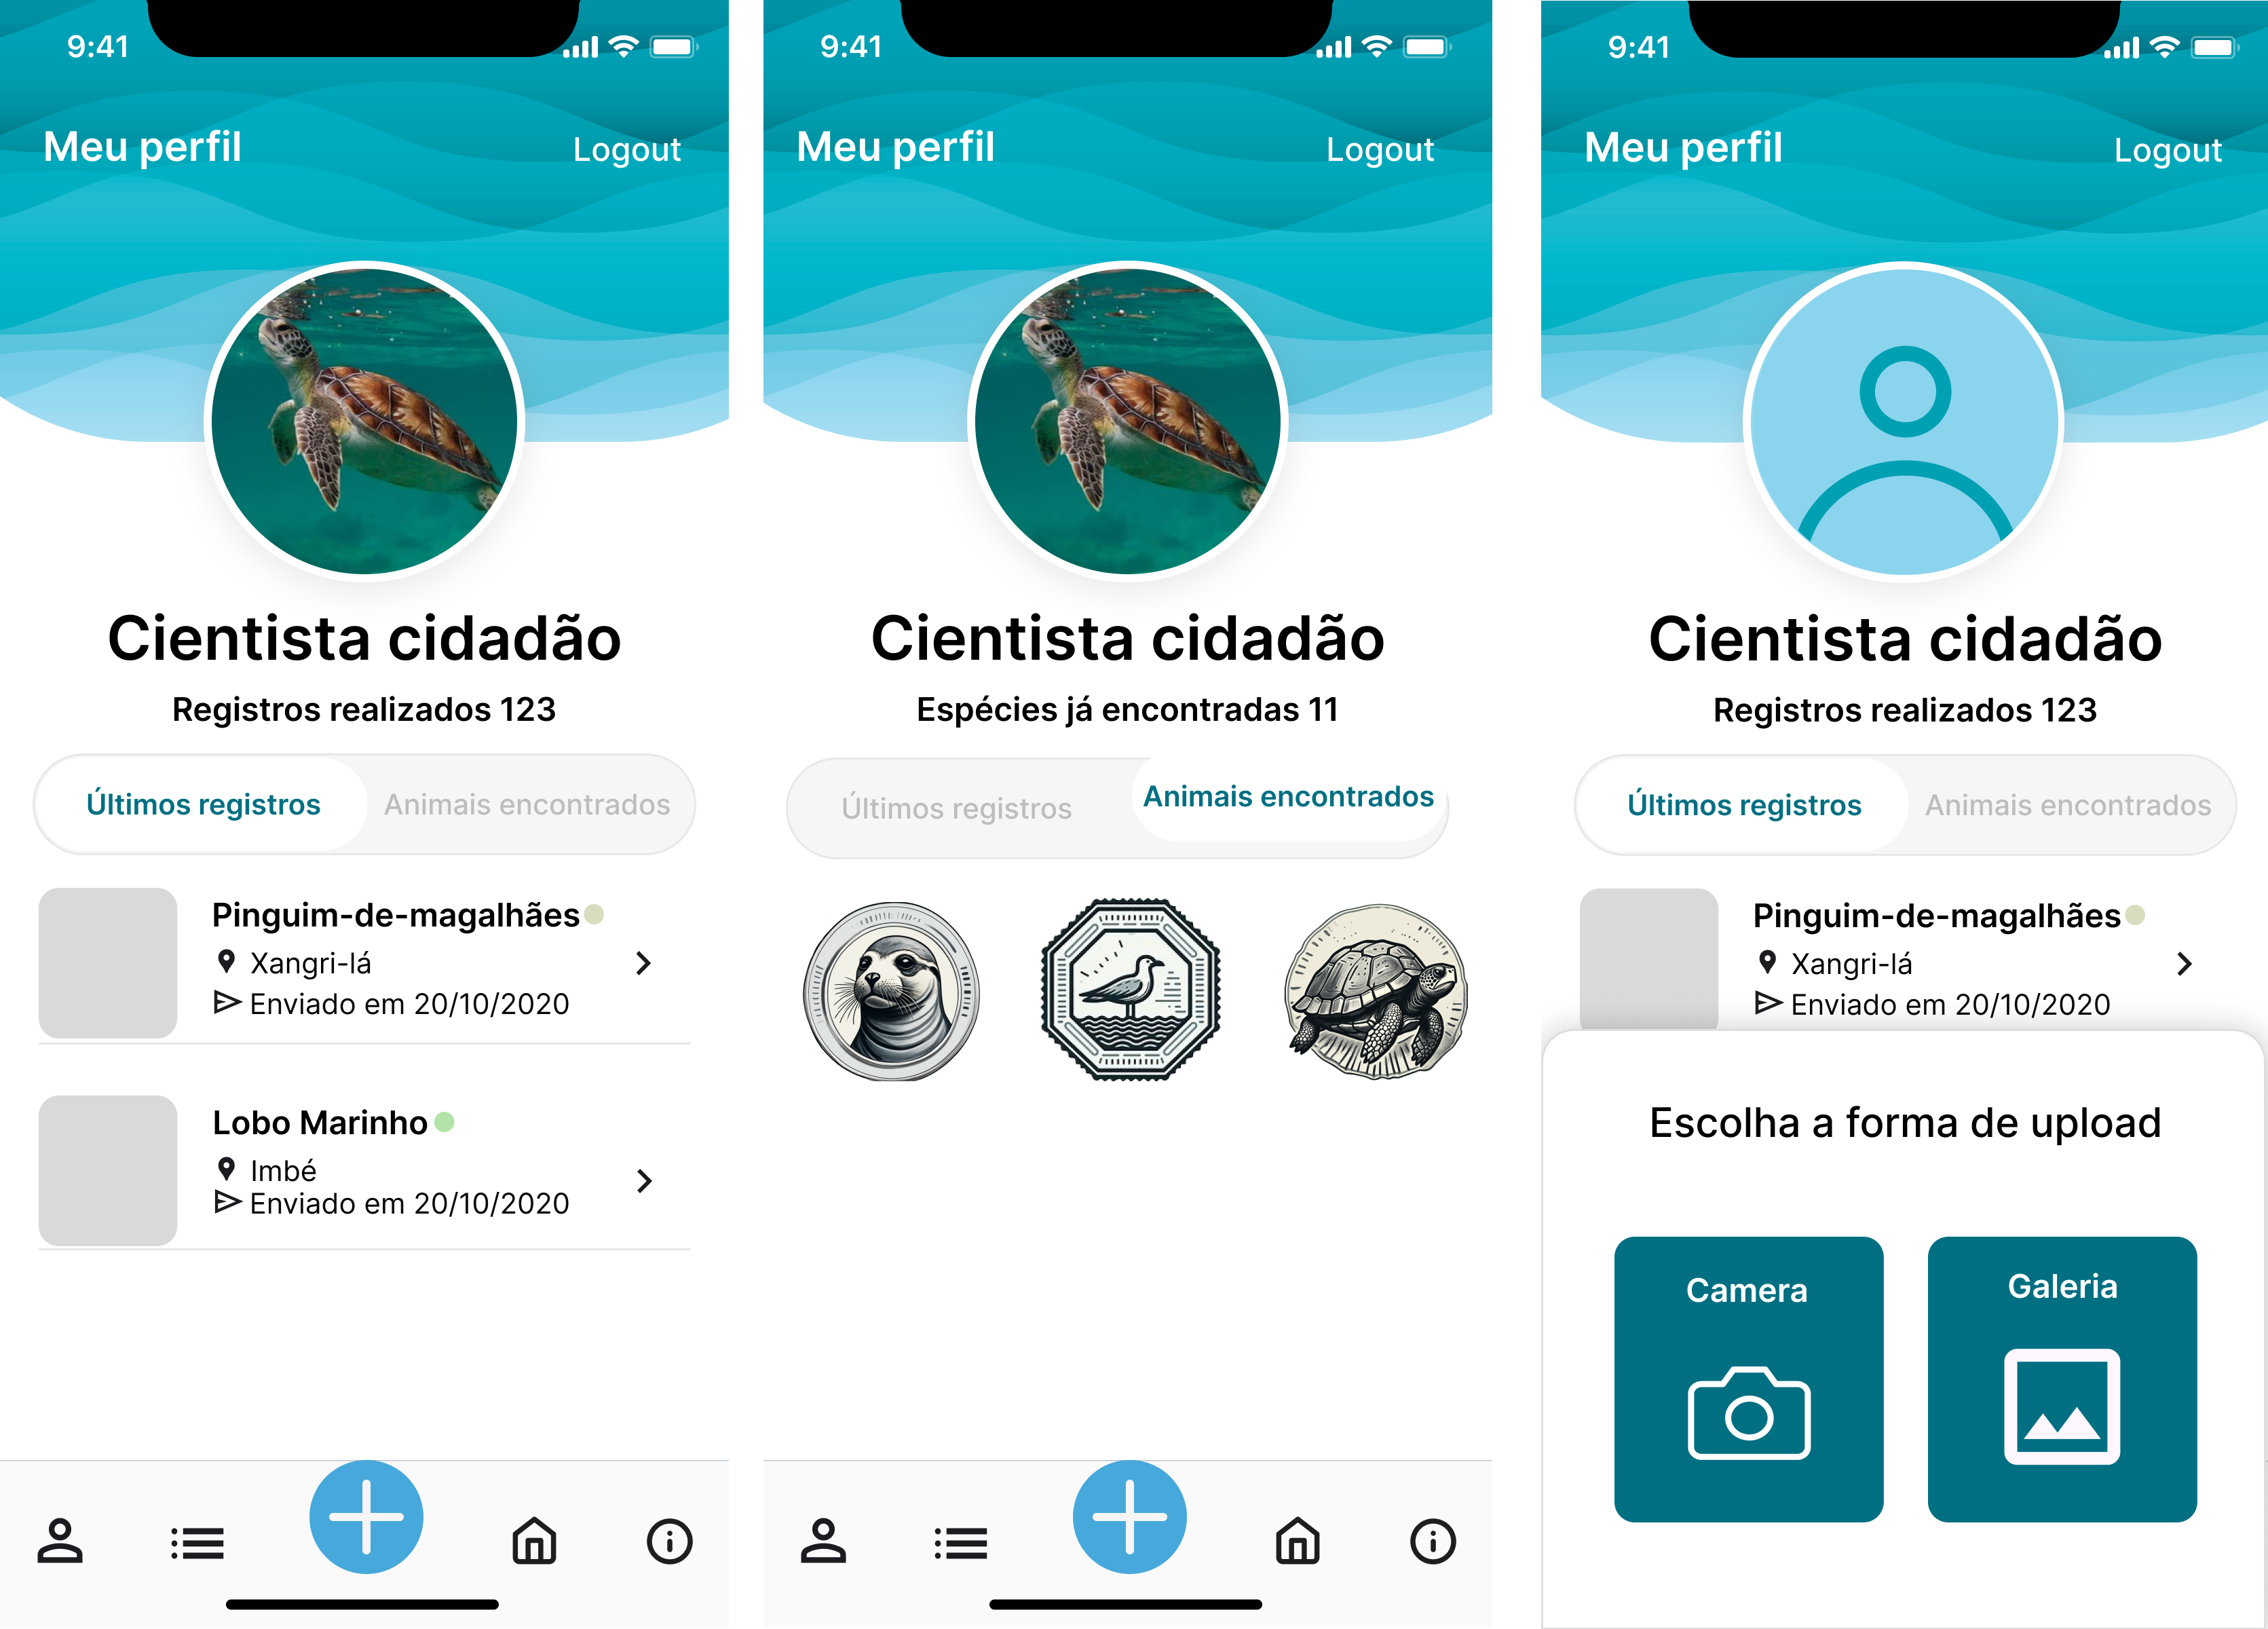
\includegraphics[height=0.53\textheight, width=\textwidth]{imagens/perfil-figma.png}
    \caption{Protótipo da tela de perfil do usuário com conquistas e histórico.}
    \label{fig:prototipo-perfil}
\end{figure}
\legend{Fonte: Autor}

As telas de fauna local (Figura~\ref{fig:prototipo-fauna-local}) seguem o mesmo padrão visual 
das demais telas do aplicativo, se assemelhando em estrutura com a de "Meus Registros" e 
"Visualizar Registro". Elas apresentam, respectivamente, uma lista de espécies e uma 
tela de detalhes com informações específicas sobre cada animal que for selecionado.

\begin{figure}[H]
    \centering
    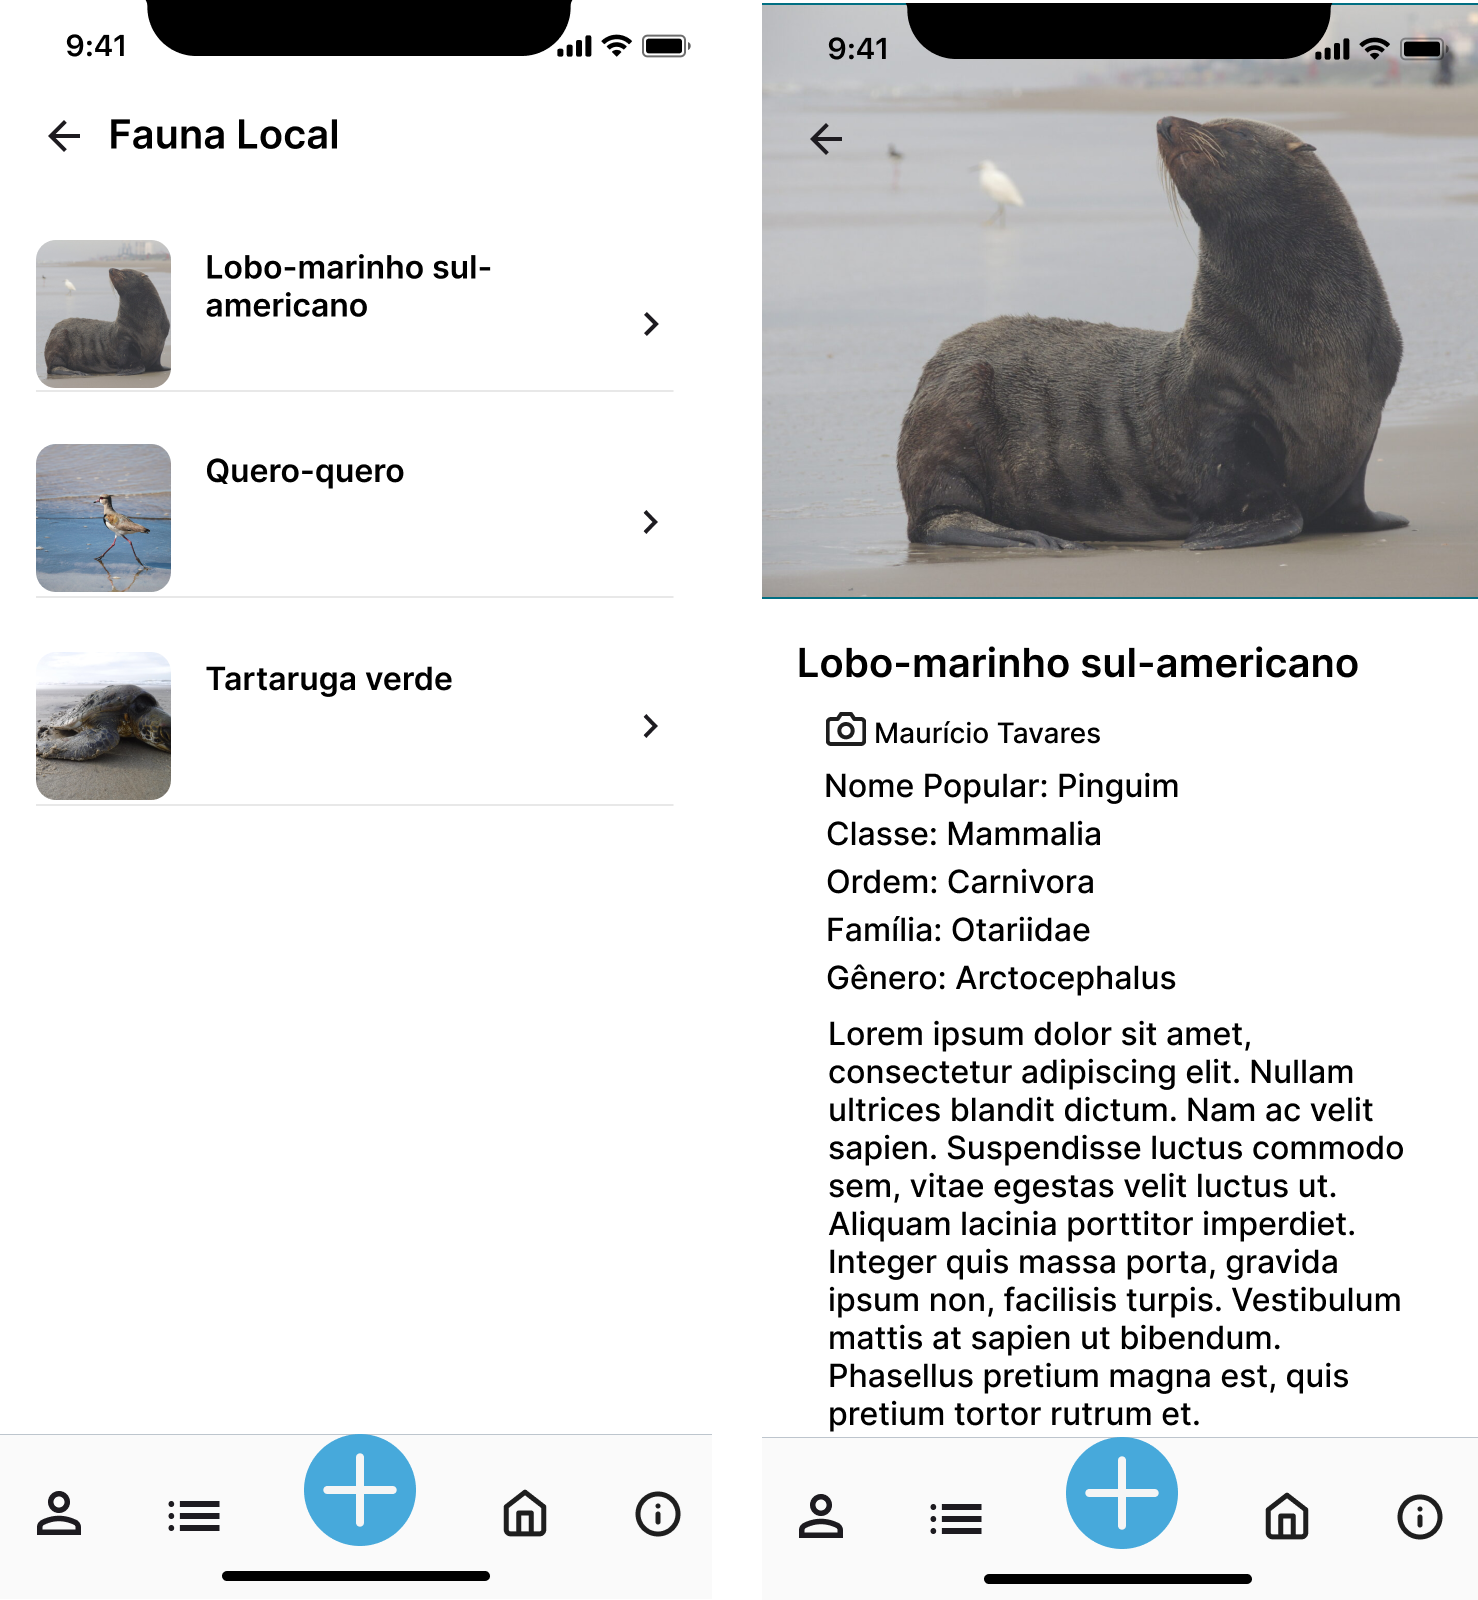
\includegraphics[height=0.6\textheight]{imagens/fauna-local-figma.png}
    \caption{Protótipo da tela de fauna local (esquerda) e detalhes da espécie (direita).}
    \label{fig:prototipo-fauna-local}
\end{figure}
\legend{Fonte: Autor}

Por fim, foi projetada a tela de recuperação de senha (Figura~\ref{fig:prototipo-esqueci-senha}), 
incluindo os estados de sucesso e de erro na validação dos campos de entrada. O padrão de erro 
apresentado nesta tela foi o mesmo utilizado em outras telas do aplicativo.

\begin{figure}[H]
    \centering
    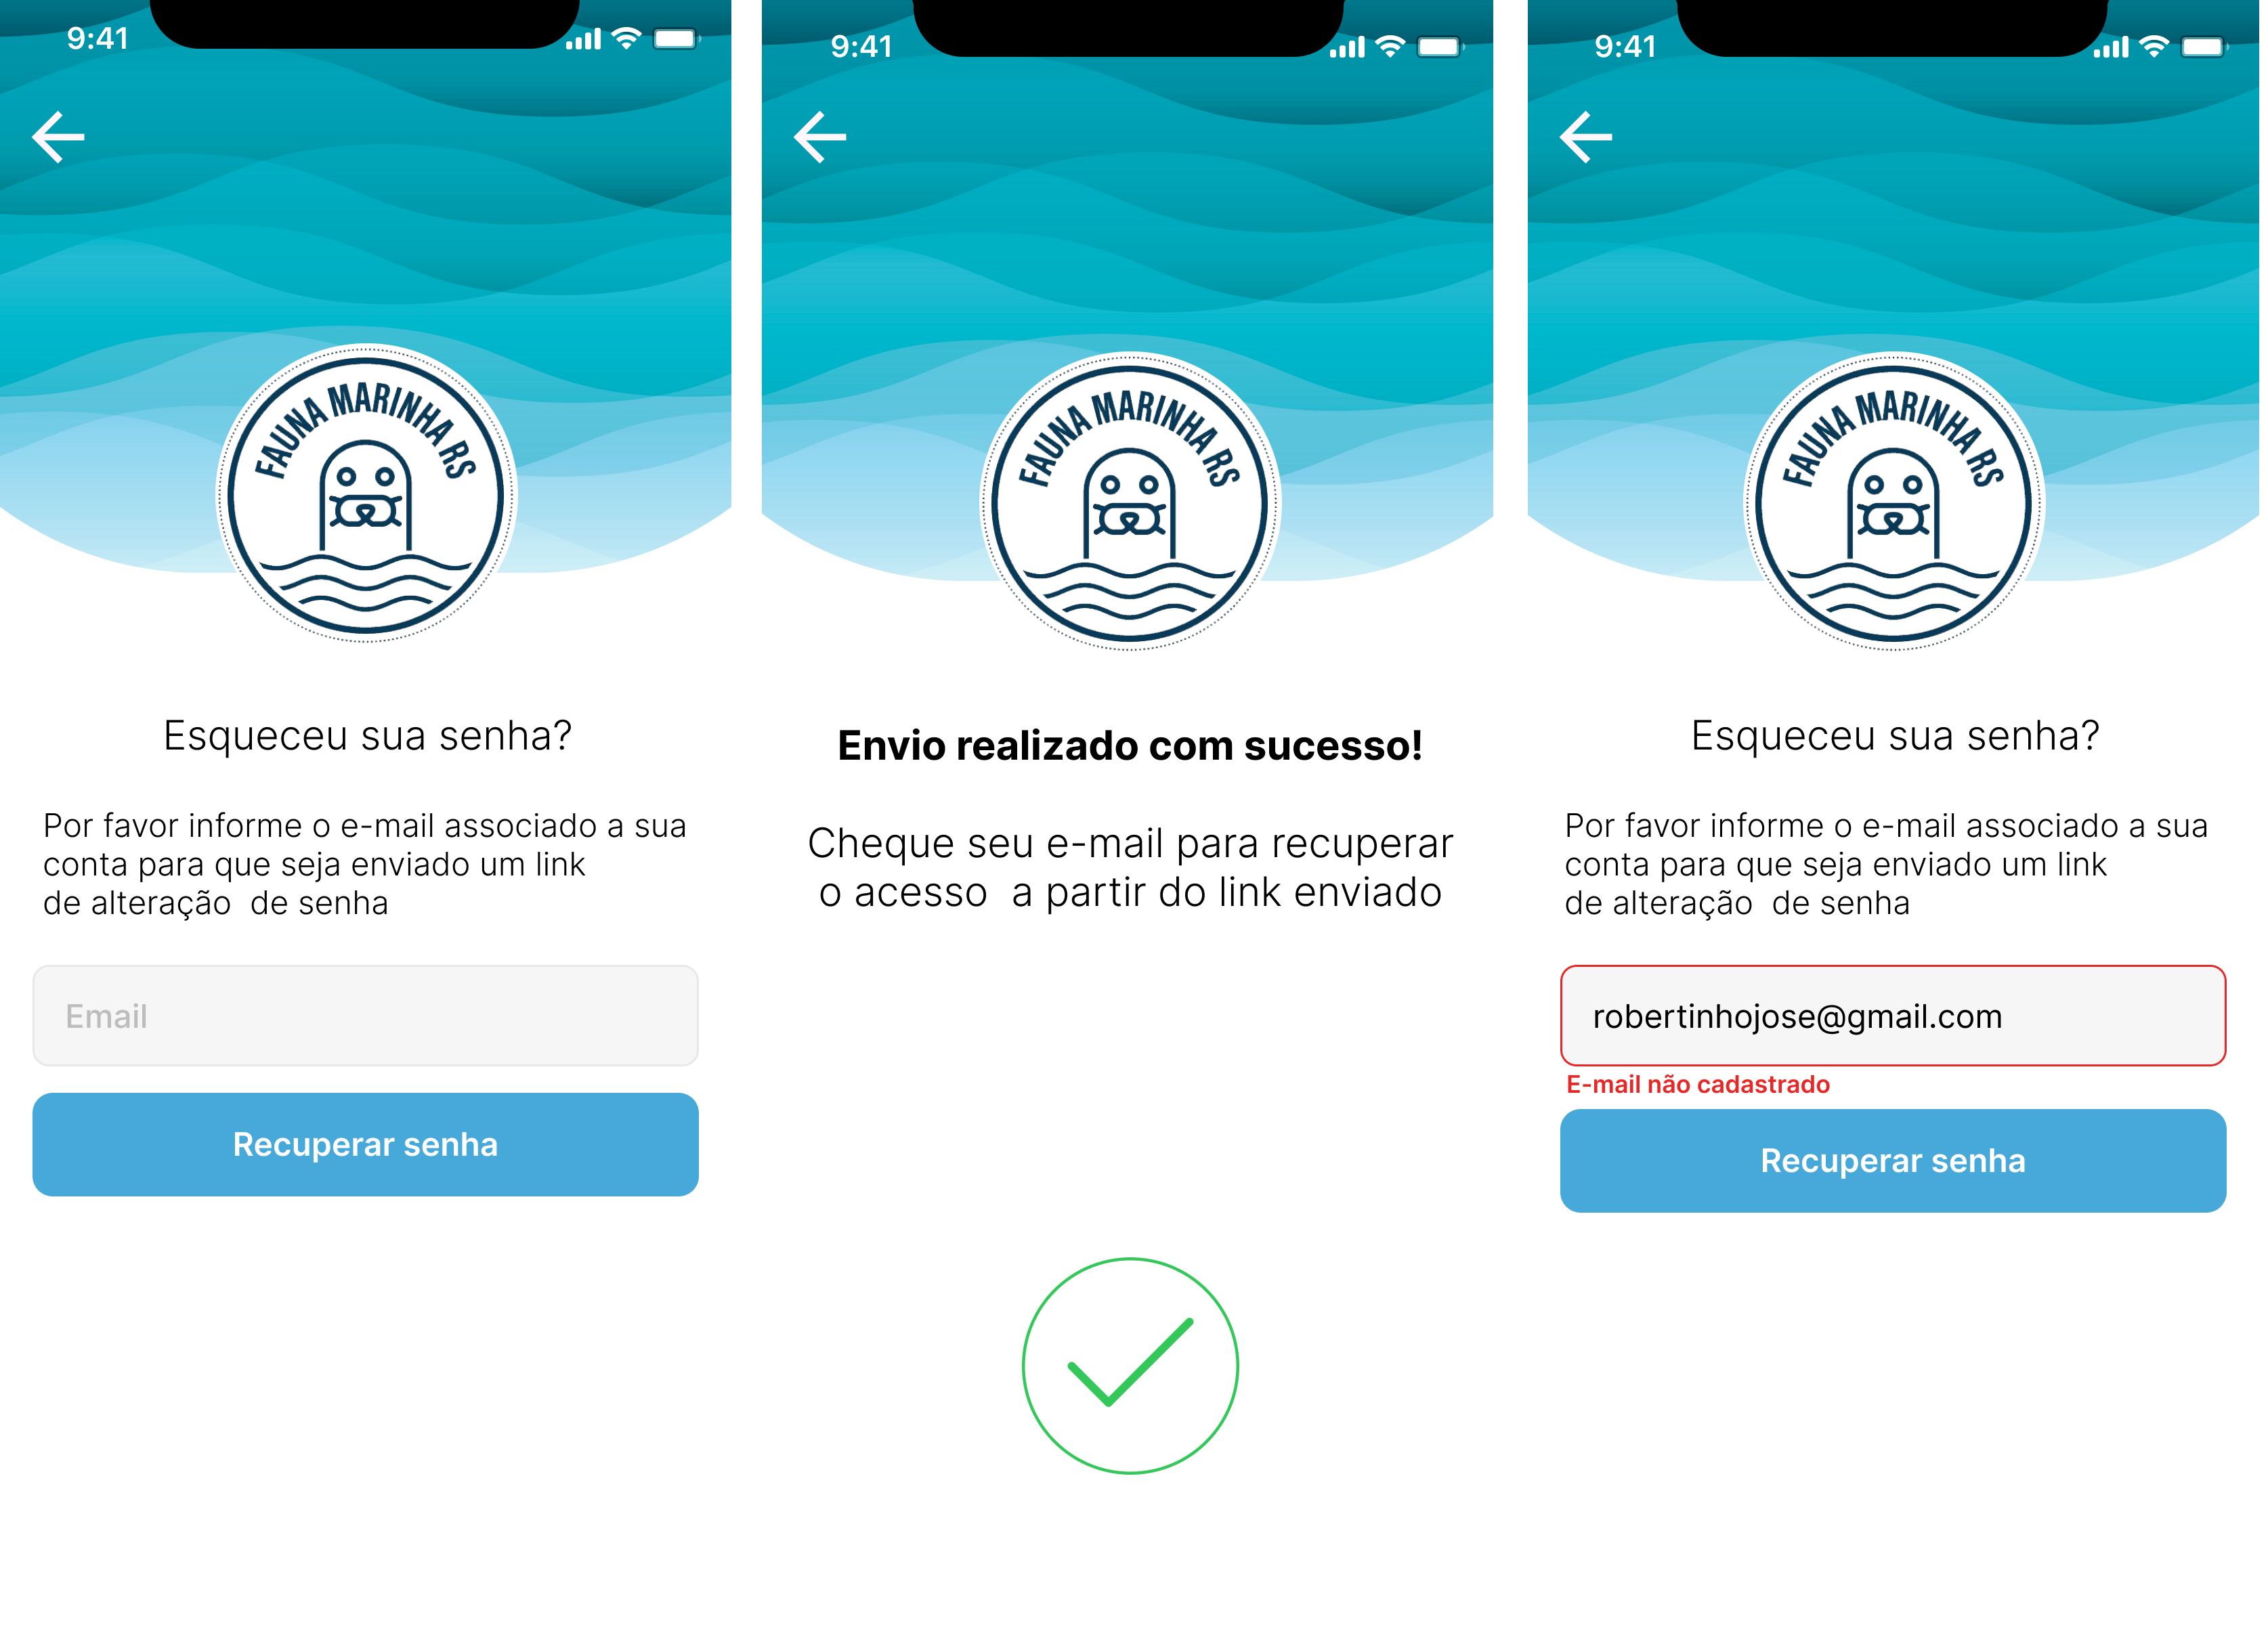
\includegraphics[height=0.53\textheight, width=\textwidth]{imagens/esqueceu-senha-figma.png}
    \caption{Protótipo da tela de recuperação de senha: formulário (esquerda), sucesso (centro) e erro de 
    validação (direita).}
    \label{fig:prototipo-esqueci-senha}
\end{figure}
\legend{Fonte: Autor}

\subsection{Desenvolvimento do Protótipo Navegável}

Utilizando a ferramenta Figma (versão gratuita \textit{online}), foi desenvolvido um
protótipo navegável de média/alta fidelidade. Essa etapa permitiu visualizar os fluxos de 
interação entre o usuário e o sistema, antecipar ajustes necessários e alinhar as funcionalidades 
às expectativas.

Foram criadas ligações interativas entre as principais telas, simulando os redirecionamentos e 
ações de navegação. O protótipo também serviu como ferramenta de validação junto a terceiros e 
como referência visual para a fase de implementação (Figura~\ref{fig:prototipo-fluxo-navegacao}).

\begin{figure}[H]
    \centering
    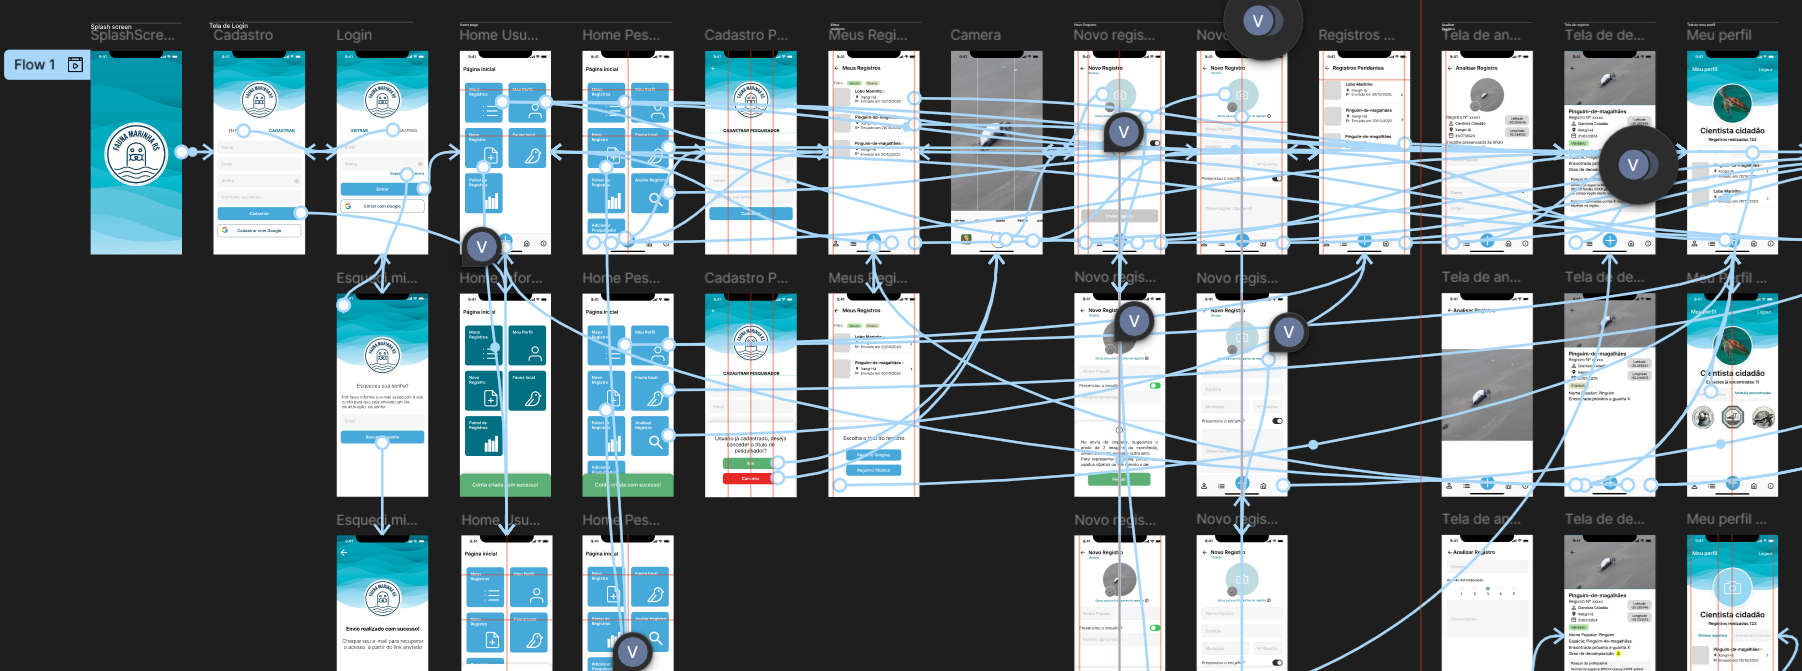
\includegraphics[width=\textwidth]{imagens/prototipo-navegavel-figma.png}
    \caption{Captura de tela do protótipo navegável desenvolvido no Figma.}
    \label{fig:prototipo-fluxo-navegacao}
\end{figure}
\legend{Fonte: Autor}

\section{Projeto Gerencial}
A gerência desse projeto foi realizada utilizando a ferramenta Jira, que possibilitou o
controle de tarefas e o acompanhamento do progresso do desenvolvimento. O fluxo de trabalho
descrito na \hyperref[sec:metodologia-desenv-software]{Seção de metodologia} deste trabalho foi 
seguido para garantir a organização e a eficiência
das tarefas. Os \textit{cards} gerados no \textit{board} foram puxados para trabalho a medida que 
havia tempo disponível para atuação. Foram catalogadas não só tarefas de codificação, como 
também tarefas de prototipação.

Foram gerados ao todo, 131 \textit{cards} desde julho de 2024 quando se deu inicio a prototipação 
da aplicação. Na Figura \ref{gra:cards-mes} é possível observar a quantidade de itens no eixo vertical
relacionada com o mês de criação no eixo horizontal. Com ele podemos concluir que os meses com 
mais entrada de demandas foram os meses de novembro de 2024, janeiro de 2025 e março de 2025,
onde o número de \textit{cards} criados foi maior que 18.

\begin{figure}[H]
    \centering
    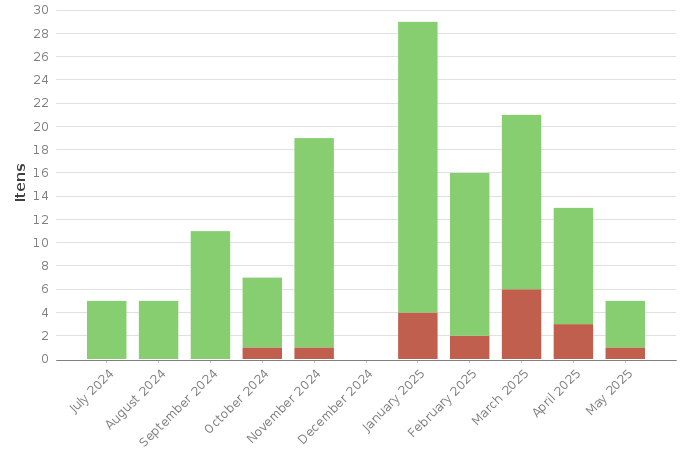
\includegraphics[width=\textwidth]{imagens/itensMes.png}
    \caption{Gráfico demonstrativo de \textit{cards} criados por mês no Jira. As 
    barras em verde representam demandas que, até a data de criação do gráfico, já haviam sido finalizadas.
    As barras em vermelho representam demandas que ainda estavam em aberto.}
    \label{gra:cards-mes}
\end{figure}
\legend{Fonte: Autor}

A Figura \ref{gra:cards-vs-resolvidos} traz uma visão cumulativa do trabalho realizado no board.
A partir dele podemos ver que, dos 131 cards criados, 113 foram concluídos, o que representa 86,26\% 
do total. Podemos observar também que, em momentos de maior atuação no projeto, a criação de 
cards está diretamente relacionada com a quantidade de cards resolvidos.
Isso está principalmente relacionado com a disponibilidade de tempo para atuar no projeto, e também
com a criação de bugs e novas demandas que surgiram durante o desenvolvimento.

\begin{figure}[H]
    \centering
    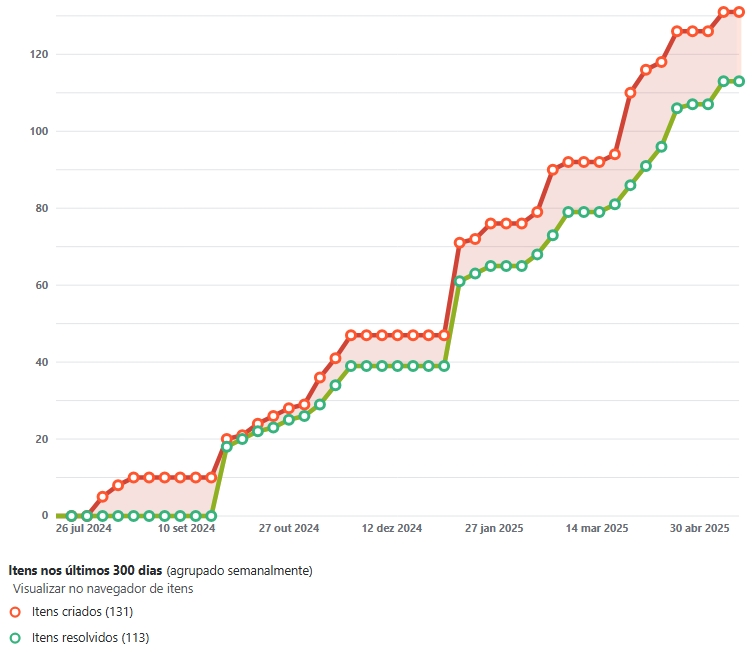
\includegraphics[width=\textwidth]{imagens/burnup-jira.jpeg}
    \caption{Gráfico demonstrativo de \textit{cards} vs resolvidos no Jira}
    \label{gra:cards-vs-resolvidos}
\end{figure}
\legend{Fonte: Autor}

A Figura~\ref{gra:tempo-medio-resolucao} apresenta o tempo médio, em dias, 
para a resolução dos \textit{cards} ao longo das semanas. É possível notar uma grande variação 
nos tempos médios, com valores baixos no período de novembro e um pico em maio de 2025. 
Esse aumento progressivo reflete a falta de atuação evidenciada no mês de dezembro vide 
Figura\ref{gra:cards-vs-resolvidos}, o aumento na complexidade das demandas e o acumulo de 
cards de melhoria no \textit{Backlog} que foram criados e não priorizados.

\begin{figure}[H]
    \centering
    \includegraphics[width=\textwidth]{imagens/tempo-médio-cards.png}
    \caption{Gráfico demonstrativo de tempo de resolução médio dos \textit{cards} por semana no Jira}
    \label{gra:tempo-medio-resolucao}
\end{figure}
\legend{Fonte: Autor}

Os \textit{cards} foram organizados em três grupos principais, que representam as diferentes
atuações necessárias para atuar em cada uma delas.
\subsection{Desenvolvimento Geral}
Esses cards representam demandas que passaram por etapas de planejamento e refinamento, 
refletindo as histórias de usuário e tarefas técnicas previstas ou requisitadas durante o desenvolvimento.
A Tabela~\ref{tab:desenv_geral_sorted} apresenta esse conjunto de funcionalidades. Ao todo foram 66 demandas
sendo 62 concluídas e 4 que ainda estão no \textit{Backlog}.

% manter essa tabela aqui ou colocar no anexo?
% talvez isso deveria ser um anexo? 

\begin{longtable}{@{}lp{7cm}ll@{}}
\caption{Registro de desenvolvimento geral (Ordenado por Data de Entrega)}\label{tab:desenv_geral_sorted}\\
\toprule
\textbf{Chave} & \textbf{Resumo} & \textbf{Status} & \textbf{Entregue} \\
\midrule
\endfirsthead

\caption{(Continuação) Registro de desenvolvimento geral (Ordenado por Data de Entrega)}\\
\toprule
\textbf{Chave} & \textbf{Resumo} & \textbf{Status} & \textbf{Entregue} \\
\midrule
\endhead

\midrule
\multicolumn{4}{r@{}}{(Continua na próxima página)} \\
\endfoot

\bottomrule
\endlastfoot

CEC-1 & Prototipação inicial das telas & Concluído & 2024-09-27 \\
CEC-2 & Tela de registro & Concluído & 2024-09-27 \\
CEC-3 & Tela de login & Concluído & 2024-09-27 \\
CEC-4 & Tela de novo registro Simples & Concluído & 2024-09-27 \\
CEC-5 & Tela de meus registros & Concluído & 2024-09-27 \\
CEC-6 & Tela de Coletanea animais & Concluído & 2024-09-27 \\
CEC-7 & Tela de perfil do usuário & Concluído & 2024-09-27 \\
CEC-8 & Tela de adicionar pesquisador & Concluído & 2024-09-27 \\
CEC-9 & Tela de esqueci minha senha & Concluído & 2024-09-27 \\
CEC-10 & Tela de selos de conquista & Concluído & 2024-09-27 \\
CEC-11 & Tela de novo registro Técnico & Concluído & 2024-09-27 \\
CEC-12 & Tela de home & Concluído & 2024-09-27 \\
CEC-13 & Tela de analisar Registro & Concluído & 2024-09-27 \\
CEC-14 & Tela de SplashScreen & Concluído & 2024-09-27 \\
CEC-15 & Tela sobre o app & Concluído & 2024-09-27 \\
CEC-16 & Codificação da SplashScreen & Concluído & 2024-09-27 \\
CEC-17 & Codificação da Tela de Registro & Concluído & 2024-09-28 \\
CEC-18 & Codificação da Tela de Login & Concluído & 2024-09-28 \\
CEC-21 & Codificação esqueci minha senha & Concluído & 2024-09-29 \\
CEC-20 & Codificação da Tela de Cadastrar Pesquisador & Concluído & 2024-10-03 \\
CEC-19 & Codificação da HomePage & Concluído & 2024-10-07 \\
CEC-22 & Adição funcionalidade de adicionar novo registro + bottom sheet & Concluído & 2024-10-09 \\
CEC-23 & Tela de registro simples & Concluído & 2024-10-15 \\
CEC-24 & Tela de registro tecnico & Concluído & 2024-10-21 \\
CEC-25 & Tela de registro controller & Concluído & 2024-10-21 \\
CEC-28 & Tela de perfil do usuário & Concluído & 2024-11-02 \\
CEC-30 & Mensagens de feedback para usuario: sucesso e erro & Concluído & 2024-11-23 \\ 
CEC-29 & Tela Meus registros & Concluído & 2024-11-03 \\
CEC-31 & Criar listas para os itens da tela de perfil & Concluído & 2024-11-03 \\
CEC-33 & Tela view de Registro & Concluído & 2024-11-08 \\
CEC-35 & Texto da tela de sobre o app & Concluído & 2024-11-16 \\
CEC-38 & Adicionar dependencia e configurar para captar a localizacao & Concluído & 2024-11-10 \\
CEC-34 & Criar montagem do registro + cadastrar registro & Concluído & 2024-11-11 \\
CEC-40 & Tela de avaliar registro & Concluído & 2024-11-15 \\
CEC-39 & Adicionar botao para remover imagem adicionada & Concluído & 2024-11-16 \\ 
CEC-42 & Funcionalidade de deletar conta & Concluído & 2024-11-23 \\
CEC-44 & Tratamento de erros do login firebase & Concluído & 2024-11-23 \\ 
CEC-41 & Adicionar badge para o icone de meus registros & Concluído & 2024-11-23 \\ 
CEC-48 & Criação do BD firebase & Concluído & 2025-01-07 \\
CEC-53 & Ordenaçao por data dos registros & Concluído & 2025-01-08 \\
CEC-59 & Adicionar skeleton de carregamento em alguns widgets & Concluído & 2025-01-09 \\
CEC-46 & Lógica de adição de pesquisador + lógica de conceder role de pesquisador pra usuário já existente & Concluído & 2025-01-10 \\
CEC-66 & Adição de uma badge para avisar registros nao visualizados & Concluído & 2025-01-11 \\
CEC-60 & Adicionar facilidade para ativar a geolocalizacao do dispositivo & Concluído & 2025-01-11 \\
CEC-78 & Skeletonizer tela inicial & Concluído & 2025-02-14 \\
CEC-98 & Geração de csv para exportação & Concluído & 2025-03-21 \\
CEC-54 & Tela painel de registros & Concluído & 2025-03-23 \\
CEC-110 & Adicionar update de localização na avaliação do registro & Concluído & 2025-03-31 \\
CEC-116 & Atualização da versão do projeto* & Concluído & 2025-03-31 \\
CEC-111 & Adicionar o campo das quaritas/ municipio para avaliar registro & Concluído & 2025-03-31 \\
CEC-118 & Adição de campo livre ponto de referencia & Concluído & 2025-04-06 \\
CEC-112 & Migraçao dos dados atuais para o firebase & Refinamento & 2025-04-06 \\
CEC-109 & Deletar registros & Concluído & 2025-04-07 \\
CEC-125 & badges para classes no perfil com contador & Concluído & 2025-04-17 \\
CEC-106 & Possibilidade de adicionar um novo animal nao presente no banco de dados quando for identificado & Concluído & 2025-04-18 \\
CEC-114 & Modificar restrições do csv & Concluído & 2025-04-18 \\
CEC-108 & Filtrar quantidade por classe & Concluído & 2025-04-18 \\
CEC-55 & Criação de badges para os animais & Concluído & 2025-04-23 \\
CEC-49 & Implementar cache dos registros enviados quando nao há internet & Concluído & 2025-05-12 \\
CEC-37 & Realizar integração front para receber dados da API baseado em criterios dos inputs & Concluído & 2025-05-12 \\
CEC-76 & Ajustes de responsividade devices menors & Concluído & 2025-05-12 \\
CEC-107 & Adicionar pedido para que a pessoa nao mostre seu rosto no informativo da foto & Concluído & 2025-05-12 \\
CEC-81 & Desenvolvimento de redirect para opção de fauna local & Concluído & 2025-05-12 \\
CEC-58 & Tela fauna local & Backlog & \\
CEC-115 & Gerar termos de uso & Backlog & \\
CEC-105 & Adicionar campo de tipo de usuário que realizou o envio do registro & Backlog & \\
CEC-113 & Mapa para marcar local aproximado no envio do registro & Backlog & \\

\end{longtable}

\subsection{Correções}
Ao longo do processo de desenvolvimento, foram identificados e registrados bugs e falhas 
de funcionamento, a origem da geração desses cards pode ser tanto de testes internos, quanto de 
validações de testadores que obtiveram alguma das builds do projeto e reportaram alguma inconsistência. 
Essas inconsistências foram tratadas por meio de cards como correções (\textit{fixes}) no ambiente Jira.

A Tabela~\ref{tab:fixes_sorted} a seguir apresenta uma relação dos 43 apontamentos dessa categoria que foram documentados, desse total, 
42 foram resolvidos e 1 ainda está no \textit{Backlog}. Isso demonstra a evolução contínua do 
sistema em busca de estabilidade e qualidade do produto final.

% manter essa tabela aqui ou colocar no anexo?

\begin{longtable}{@{}lp{7cm}ll@{}}
\caption{Registro de Correções (Fixes) (Ordenado por Data de Entrega)}\label{tab:fixes_sorted}\\
\toprule
\textbf{Chave} & \textbf{Resumo} & \textbf{Status} & \textbf{Entregue} \\
\midrule
\endfirsthead

\caption{(Continuação) Registro de Correções (Fixes) (Ordenado por Data de Entrega)}\\
\toprule
\textbf{Chave} & \textbf{Resumo} & \textbf{Status} & \textbf{Entregue} \\
\midrule
\endhead

\midrule
\multicolumn{4}{r@{}}{(Continua na próxima página)} \\
\endfoot

\bottomrule
\endlastfoot

CEC-61 & Fix: Feedback para o usuario quando um registro offline é enviado & Concluído & 2025-01-10 \\
CEC-67 & Fix: Ajustes de condicionais de tela de avaliar registro & Concluído & 2025-01-11 \\
CEC-65 & Fix: Mensagem de não adição de imagem & Concluído & 2025-01-11 \\
CEC-69 & Fix: Ajuste de envio da imagem independente do input escolhido & Concluído & 2025-01-11 \\
CEC-63 & Fix: Adicionar um icone X no input de dropdown para deletar o conteudo & Concluído & 2025-01-11 \\
CEC-36 & Fix: Mensagem de dicas para fotografia & Concluído & 2025-01-11 \\
CEC-71 & Fix: Deletar foto de perfil quando conta é deletada & Concluído & 2025-01-11 \\
CEC-62 & Fix: Ajustar visualização de filtros para ser mais intuitivo & Concluído & 2025-01-11 \\
CEC-56 & Fix: Ajuste do header registros pendentes + meus registros & Concluído & 2025-01-17 \\
CEC-77 & Fix: Ajuste dos cards de meus registros (responsividade) & Concluído & 2025-01-23 \\
CEC-92 & Fix: Ajuste de italico na apresentação da taxonomia & Concluído & 2025-02-22 \\
CEC-95 & Fix: Alterar a quantidade de caracteres do campo obs para 600 + travar escrita & Concluído & 2025-02-22 \\
CEC-83 & Fix: Ajuste no regex de cadastro do campo de nome popular & Concluído & 2025-02-22 \\
CEC-94 & Fix: Ajuste de campos opcionais que estao sendo apresentados como obrigatorios no envio da avaliacao do registro & Concluído & 2025-02-22 \\
CEC-88 & Fix: A partir da localizacao do registro adicionar o campo nome da cidade & Concluído & 2025-02-23 \\
CEC-90 & Fix: Na tela de registro simples, permitir que o usuario adicione a cidade e a guarita & Concluído & 2025-02-23 \\
CEC-86 & Fix: Alteração do gráfico em pontos por gráfico em barras tela de painel de registros & Concluído & 2025-02-23 \\
CEC-99 & Fix: Campo de obs nao está sendo mantido & Concluído & 2025-03-21 \\
CEC-102 & Fix: Botão voltar tela de registros avaliados & Concluído & 2025-03-23 \\
CEC-100 & Fix: Loading da image do bottomsheet mapa & Concluído & 2025-03-24 \\
CEC-117 & Fix: Limpar dados de guarita municipio & Concluído & 2025-04-01 \\
CEC-119 & Fix: Ajustar aparecimento dos botoes de avaliar registro + adicionar pesquisador & Concluído & 2025-04-05 \\
CEC-121 & Fix: Validaçao de liberar envio de registros & Concluído & 2025-04-06 \\
CEC-101 & Fix: Loading entrar com Google ausente & Concluído & 2025-04-06 \\
CEC-127 & Fix: Ajuste na visualizacao do retorno do profissional na tela de register view & Concluído & 2025-04-17 \\
CEC-126 & Fix: Ajuste de estado inicia do seletor dde avaliar registro & Concluído & 2025-04-17 \\
CEC-128 & Fix: Classe no model de AnimalResponse & Concluído & 2025-04-18 \\
CEC-131 & Fix: Overflow do nome na tela de perfil & Concluído & 2025-04-18 \\
CEC-132 & Fix: Problema no envio de registro offline sem localização & Concluído & 2025-05-06 \\
CEC-133 & Fix: Validacao dos campos registros simples & Concluído & 2025-05-06 \\
CEC-134 & Fix: Ajuste de mostrar registros de guaritdas no mapa & Concluído & 2025-05-06 \\
CEC-136 & Fix: Formatacao de coordenadas quando randomizador de guarita é acionadio & Concluído & 2025-05-06 \\
CEC-43 & Fix: Arrumar redirect após o cadastro & Concluído & 2025-05-12 \\
CEC-50 & Fix: Alteração semantica do campo de genero & Concluído & 2025-05-12 \\
CEC-51 & Fix: Ajustes propostos pela professora Karen & Concluído & 2025-05-12 \\
CEC-52 & Fix: Comportamento do dropdown dos inputs de pesquisa & Concluído & 2025-05-12 \\
CEC-68 & Fix: Ajustes de condicionais da tela de visualizar registro & Concluído & 2025-05-12 \\
CEC-75 & Fix: Adicionar lógica de contador de animais encontrados após avaliações & Concluído & 2025-05-12 \\
CEC-79 & Fix: Lógica para permitir acesso a features offline HomePage & Concluído & 2025-05-12 \\
CEC-130 & Fix: Ajuste de bloqueio de switch quando gps esta desligado & Concluído & 2025-05-12 \\
CEC-82 & Fix: Ajuste no datePicker register pannel & Concluído & 2025-05-12 \\
CEC-85 & Fix: Ajuste no tamanho do campo de observacao e retorno do profissional & Concluído & 2025-05-12 \\
CEC-80 & Fix: Enviar e manipular o switch permite duplicar o registro & Concluído & 2025-05-12 \\
CEC-104 & Fix: Campo de busca quando apagado deve apresentar todas as opcoes novamente & Backlog & \\

\end{longtable}


\subsection{Débitos Técnicos e Melhorias}
Além das funcionalidades previstas e dos \textit{bugs} encontrados, também foram abertos \textit{cards} 
para apontamentos de melhorias para algumas funcionalidades e respostas do sistema e débitos técnicos produzidos 
durante a codificação. 
Esses pontos surgiram durante a implementação de funcionalidades, revisões de código ou testes 
exploratórios e regressivos.

A Tabela~\ref{tab:dt_melhorias_sorted} apresenta as melhorias e ajustes técnicos catalogados, 
evidenciando práticas de refatoração e aprimoramento contínuo. Ao todo foram 19 \textit{cards} abertos com esse intuito,
dos quais 8 foram resolvidos e 11 ainda estão no \textit{Backlog}.

% manter essa tabela aqui ou colocar no anexo?
% talvez isso deveria ser um anexo? 
\begin{longtable}{@{}lp{7cm}ll@{}}
\caption{Registro de Débitos Técnicos e Melhorias (Ordenado por Data de Entrega)}\label{tab:dt_melhorias_sorted}\\
\toprule
\textbf{Chave} & \textbf{Resumo} & \textbf{Status} & \textbf{Entregue} \\
\midrule
\endfirsthead

\caption{(Continuação) Registro de Débitos Técnicos e Melhorias (Ordenado por Data de Entrega)}\\
\toprule
\textbf{Chave} & \textbf{Resumo} & \textbf{Status} & \textbf{Entregue} \\
\midrule
\endhead

\midrule
\multicolumn{4}{r@{}}{(Continua na próxima página)} \\
\endfoot

\bottomrule
\endlastfoot
CEC-74 & Melhoria: Adicionar um marcador nos registros que ainda nao foram visualizados na tela de meus registros & Concluído & 2024-11-23\\
CEC-73 & Melhoria: Poder abrir a imagem na tela de visualizar registro & Concluído & 2025-01-11 \\
CEC-70 & Melhoria: Melhorar carregamento das imagens nas telas que apresentam todos os registros & Concluído & 2025-01-11 \\
CEC-123 & Melhoria: Alterar nome de salvamento das imagens dos registros & Concluído & 2025-04-07 \\
CEC-129 & Melhoria Adicionar loading no botao de avaliar registro & Concluído & 2025-04-18 \\
CEC-87 & Melhoria: Captar localizacao de uma imagem da galeria quando presente & Concluído & 2025-05-12 \\
CEC-32 & Melhoria: Ajustar centralização da lista de badges na tela de perfil & Concluído & 2025-05-12 \\
CEC-96 & Melhoria: Adicionar switch para envio de imagens da galeria tela de registro técnico & Concluído & 2025-05-12 \\
CEC-93 & Melhoria: Adicionar pré cadastro dos municpios do litoral norte, apenas seleção & Concluído & 2025-05-12 \\
CEC-45 & Melhoria: Modificar logica de tratamento de exceptions para remocao da passagem de BuildContext & Backlog &  \\
CEC-124 & Melhoria: Notificação quando registro é avaliado & Backlog & \\
CEC-122 & Melhoria: Exception de email nao encontrado & Backlog & \\
CEC-137 & Melhoria: Lógica de retry quando a internet está ruim & Backlog & \\
CEC-91 & Melhoria: Glossário ilustrado dos principais animais & Backlog & \\
CEC-57 & Melhoria: Validação de email cadastrado esqueci minha senha & Backlog & \\
CEC-120 & Melhoria: Criar uma thumb com a imagem dos registros no mapa do painel & Backlog & \\
CEC-26 & Melhoria: Refac da navegação & Backlog & \\
CEC-97 & Fix: Alteracao da ordem dos campos do formulário de avaliar registro & Backlog & \\
CEC-72 & Fix: Ajustar lógica de visualização da foto de perfil & Backlog & \\
CEC-103 & Fix: Pop up informando saída do app no botao de fauna local & Backlog & \\

\end{longtable}



\section{Implementação do Sistema}
% descrever a implementação do sistema, com detalhes técnicos e decisões de projeto.
% fazer relações com o projeto gerencial e com os requisitos funcionais e não funcionais.
Nesta seção, iremos abordar a codificação do aplicativo e apresentar o produto final gerado após  
as entrevistas, desenvolvimento, ajustes de funcionamento e correções de \textit{bugs}.

O aplicativo FaunaMar foi desenvolvido utilizando uma arquitetura modular baseada no padrão \textit{MVC} 
(Model-View-Controller), que promove a separação clara entre as responsabilidades da aplicação. 
A camada Model sendo responsável pelos dados e pela comunicação com o banco, enquanto a View, trata 
da interface e interação com o usuário e a Controller gerencia a lógica de negócio e coordena a 
comunicação entre as outras duas. Além disso, foram desenvolvidos widgets personalizados reutilizáveis, 
aplicados em diversos pontos da interface, com o objetivo de padronizar elementos visuais e reduzir a 
duplicação de código facilitando alterações na interface. Essa estrutura segue princípios fundamentais 
da engenharia de software, como coesão, baixo acoplamento e reutilização de componentes, o 
que contribui para a escalabilidade do sistema e a manutenção do código.

As funcionalidades do sistema foram construídas de maneira independente,
permitindo que as alterações e melhorias possam ser implementadas de forma isolada, 
sem impactar outras partes do sistema. Existem dois tipos de usuários no sistema, os usuários comuns, 
chamados de cientistas cidadãos, e os pesquisadores, que são os profissionais que validam os dados 
enviados. 

As principais seções do aplicativo incluem:

\begin{itemize}
    \item \textbf{Login/Cadastro:} autenticação e criação de contas de usuários;
    \item \textbf{Menu Inicial:} tela de acesso rápido às funcionalidades principais;
    \item \textbf{Envio de Registros:} seção destinada ao cadastro de novos avistamentos de fauna, é possível enviar dois tipos de registros, um simples e outro técnico;
    \item \textbf{Painel de Registros:} seção que centraliza informações sobre os registros enviados, permitindo visualização, filtragem e exportação de dados;
    \item \textbf{Meus Registros:} seção onde o usuário pode acompanhar e gerenciar os registros enviados por ele;
    \item \textbf{Avaliar Registro:} seção exclusiva para pesquisadores, para análise e validação de dados enviados por todos os usuários;
    \item \textbf{Fauna Local:} catálogo externo de espécies da fauna marinha local;
    \item \textbf{Meu Perfil:} seção de visualização e edição de informações pessoais do usuário;
    \item \textbf{Adicionar Pesquisador:} seção exclusiva para pesquisadores, permitindo a inclusão de novos usuários com perfil de pesquisador;
    \item \textbf{Sobre o app:} informações sobre a versão e créditos do projeto.
\end{itemize}

A seguir, cada uma dessas seções será apresentada com suas respectivas telas, fluxos de interação, 
decisões de projeto e aspectos técnicos sobre o funcionamento do sistema.

\subsection{Splashscreen}
Foi gerada uma \textit{splashscreen} para o aplicativo, essa tela traz o logo do projeto 
Fauna Marinha RS e é apresentada durante o carregamento completo do aplicativo 
para que o usuário tenha um feedback visual de que o aplicativo está sendo iniciado (Figura~\ref{fig:splashscreen}).

\begin{figure}[H]
    \centering
    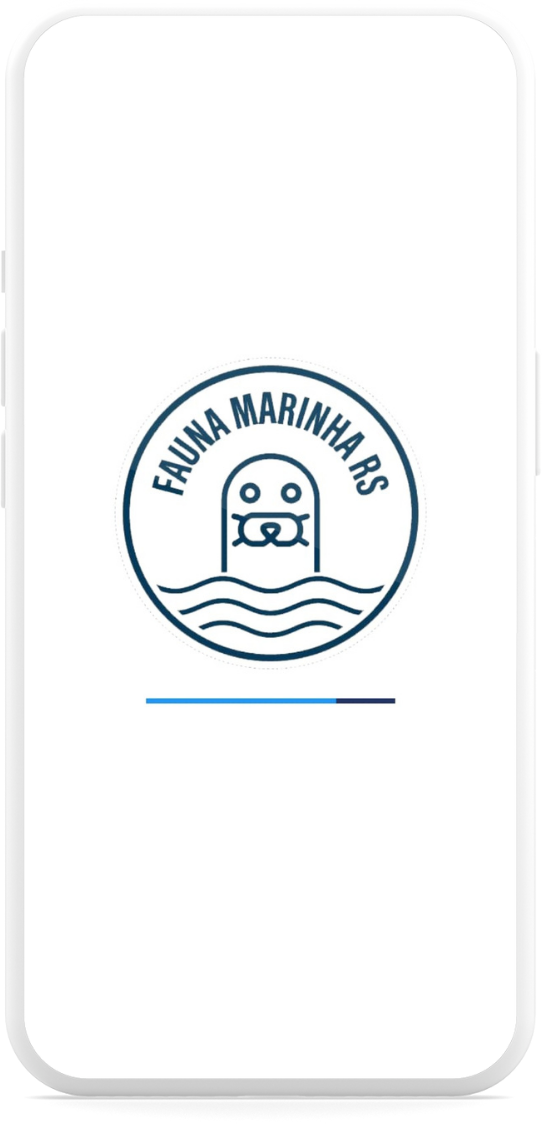
\includegraphics[width=0.5\textwidth]{imagens/sistema/device_frame/splashscreen.png}
    \caption{\textit{Splashscreen} do aplicativo.}
    \label{fig:splashscreen}
\end{figure}
\legend{Fonte: Autor}

\subsection{Login e Cadastro}
Após a \textit{splashscreen}, caso o usuário não tenha feito login previamente, ele 
é direcionado para a tela de login. Esta tela apresenta as seguintes opções: login com e-mail e senha, login via 
conta Google, realizar cadastro e recuperar senha (Figura~\ref{fig:login}).

A Figura~\ref{fig:fluxo-login-cadastro} apresenta o diagrama de fluxo que resume o processo de autenticação 
do aplicativo, abrangendo os principais caminhos possíveis, como login com diferentes provedores, 
recuperação de senha e cadastro de novos usuários. Esse diagrama auxilia na compreensão geral 
da navegação inicial e da lógica de acesso implementada no sistema.

\begin{figure}[H]
    \centering
    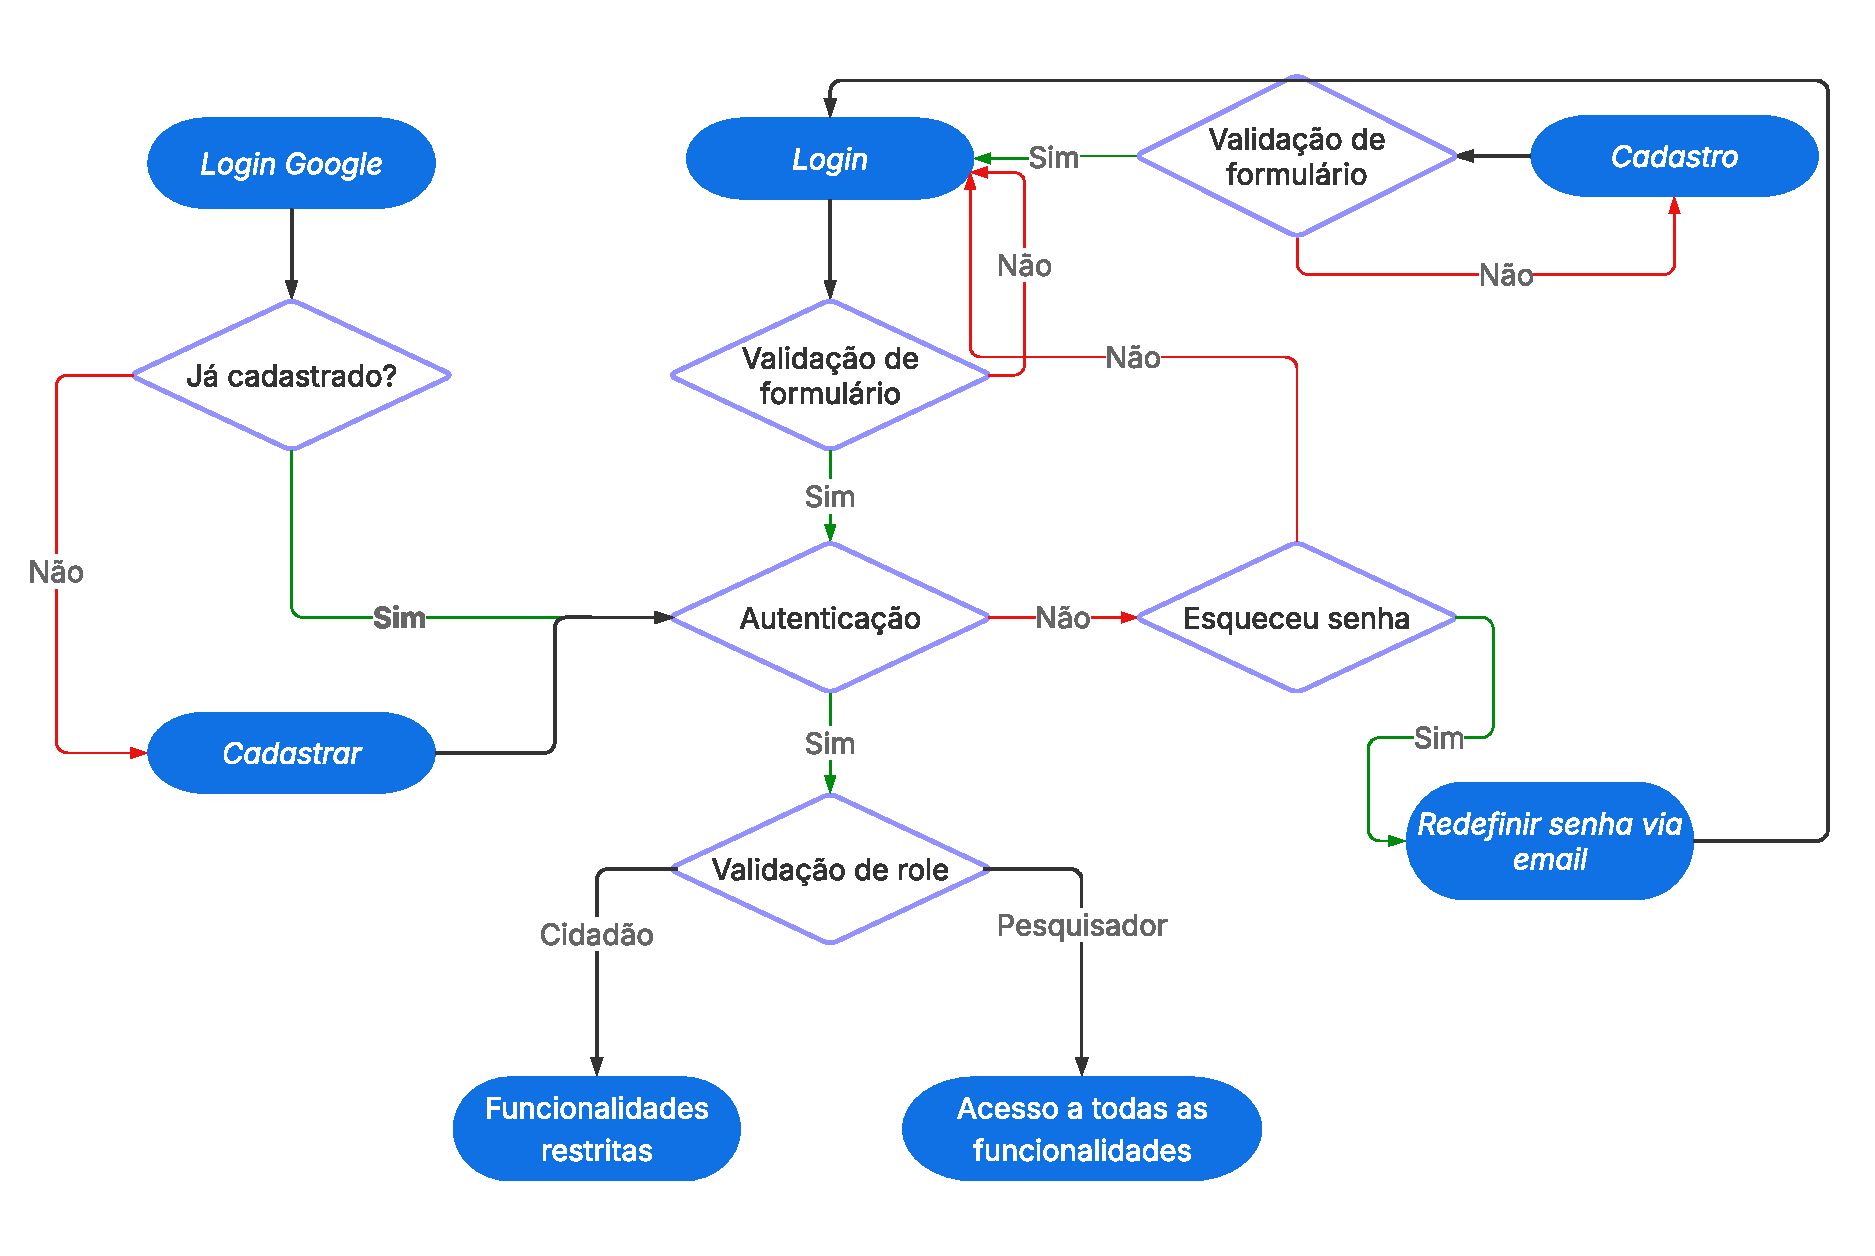
\includegraphics[width=1\textwidth]{diagrams/fluxograma_login-cadatro.pdf}
    \caption{Diagrama de fluxo do processo de autenticação e cadastro no aplicativo.}
    \label{fig:fluxo-login-cadastro}
\end{figure}
\legend{Fonte: Autor}

Em ambos os provedores de login, o processo de autenticação é realizado por meio do Firebase Authentication,
para garantir a segurança e a privacidade dos dados do usuário. A autenticação via Google
é implementada utilizando o pacote \texttt{google\_sign\_in}, que permite integração com a conta Google do usuário, 
facilitando o acesso ao aplicativo. O forumulário de login possui validações para garantir que o usuário
informe um e-mail em formato válido (com "@" e ".com"), e uma senha que atenda o padrão esperado (Figura~\ref{fig:login-erro}).

\begin{figure}[H]
    \centering
    \begin{minipage}[t]{0.48\textwidth}
        \centering
        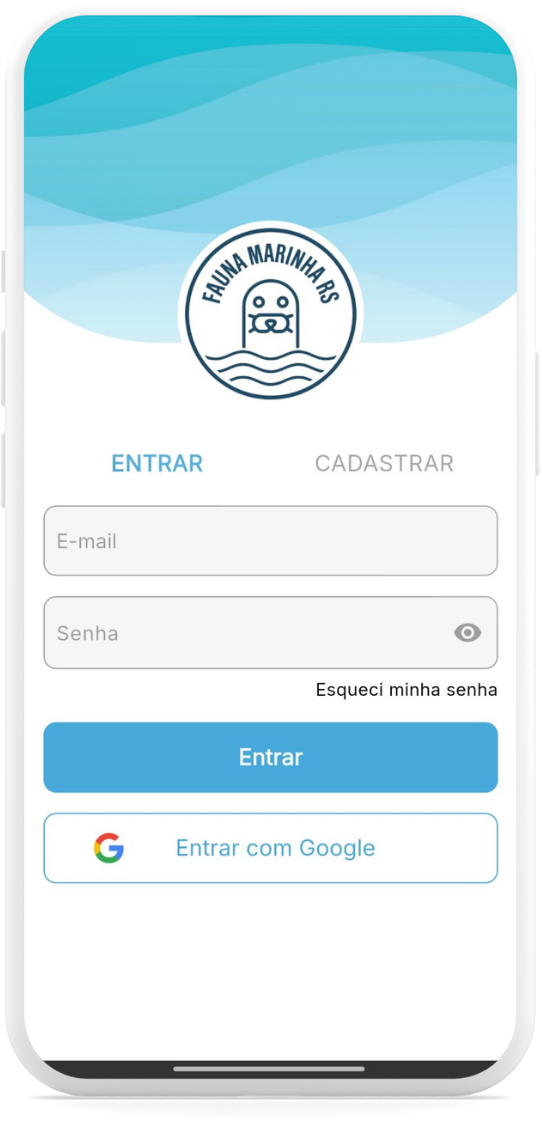
\includegraphics[height=0.72\textheight]{imagens/sistema/device_frame/login.png}
        \caption{Tela de login com formulário de entrada.}
        \label{fig:login}
    \end{minipage}
    \hfill
    \begin{minipage}[t]{0.48\textwidth}
        \centering
        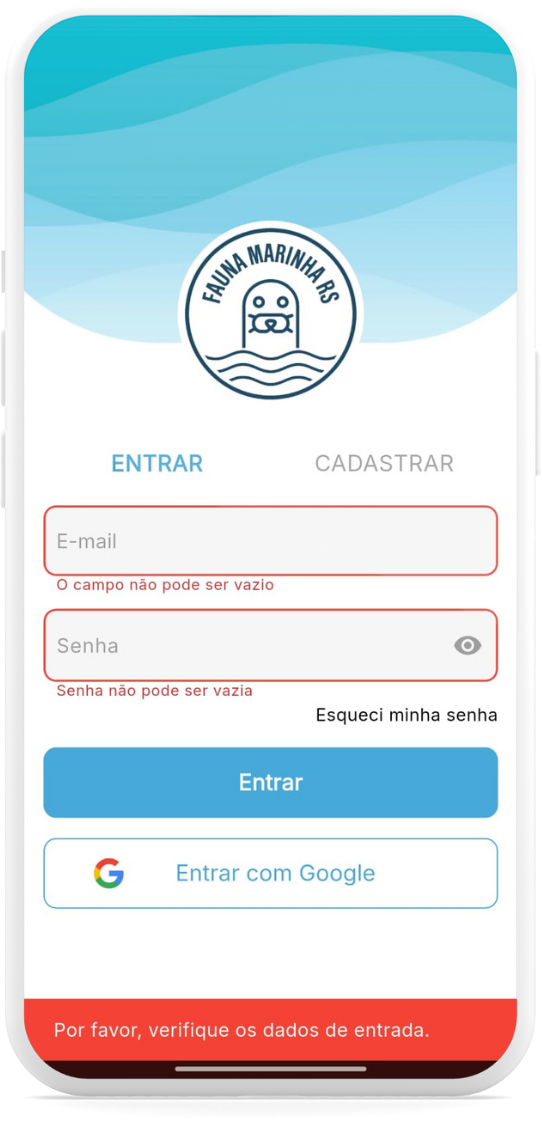
\includegraphics[height=0.72\textheight]{imagens/sistema/device_frame/formularioLogin_erro.png}
        \caption{Exemplo de erro de validação do formulário de login.}
        \label{fig:login-erro}
    \end{minipage}
\end{figure}
\legend{Fonte: Autor}

O Firebase Authentication utiliza uma versão internamente modificada do algoritmo \textit{Scrypt} 
para realizar o \textit{hash} das senhas dos usuários \cite{firebaseScrypt2023}. Durante o processo de registro, 
ao criar uma senha, o sistema aplica uma função de \textit{hash} criptográfica à senha fornecida, gerando uma sequência 
de caracteres única, conhecida como \textit{hash}. Segundo \citeonline{Serafim2012}, “o \textit{hash} é irreversível. Não 
há informação suficiente no valor do \textit{hash} h para recuperar a mensagem m”, o que assegura que a senha 
original não possa ser obtida a partir do valor armazenado. Essa abordagem está em conformidade com a Lei Geral 
de Proteção de Dados (LGPD), que exige que dados pessoais, como senhas, sejam tratados de 
forma segura e responsável \cite{BRASIL2018lgpd}.

Apenas o \textit{hash} gerado é armazenado no banco de dados, vinculado ao identificador do usuário. No momento do login, 
a senha fornecida é novamente processada pela mesma função de \textit{hash} e comparada ao valor armazenado. Caso os dois 
hashes coincidam, a autenticação é concluída com sucesso, caso contrário, o acesso é negado.

Para evitar duplicidade de contas e oferecer maior flexibilidade ao usuário, optou-se pela utilização da 
funcionalidade de vinculação de contas do Firebase. Essa funcionalidade permite que, 
quando um usuário tenta se autenticar com um provedor (por exemplo, e-mail e senha) usando um endereço de 
e-mail que já está associado a outro provedor (como o Google Sign-In), 
o Firebase automaticamente une esses métodos de login em uma única chave de usuário.

Caso o usuário tenha esquecido a senha, ele pode solicitar a recuperação por meio do e-mail cadastrado.
Para isso, o usuário deve clicar em "Esqueci minha senha" na tela de login, que irá realizar o 
redirecionamento para a tela de recuperação de senha (Figura~\ref{fig:esqueci-senha}). Após a inserção e validação 
do e-mail, o aplicativo envia um e-mail de recuperação com um link seguro para redefinir a senha 
(Figuras~\ref{fig:email-esqueci-senha-sucesso} e ~\ref{fig:email-esqueci-senha}). Todo esse processo 
é realizado utilizando métodos do Firebase Authentication, que permite gerenciar o envio do e-mail e realiza 
o processo de substituição da senha antiga pela nova.

\begin{figure}[H]
        \centering
        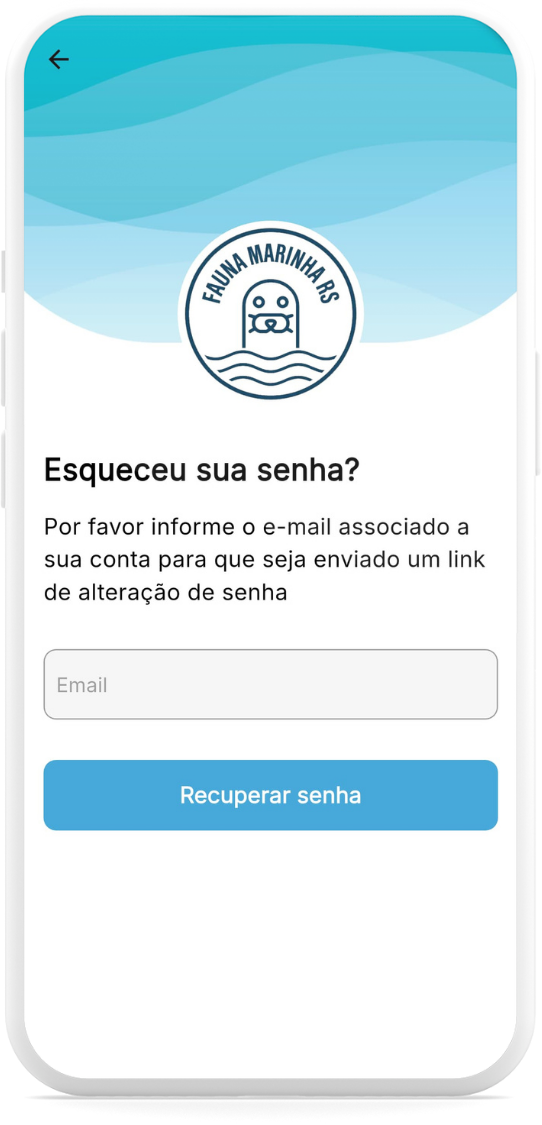
\includegraphics[height=0.72\textheight]{imagens/sistema/device_frame/recuperarSenha.png}
        \caption{Tela de recuperação de senha.}
        \label{fig:esqueci-senha}
\end{figure}
\legend{Fonte: Autor}

\begin{figure}[H]
    \centering
    \begin{minipage}[t]{0.48\textwidth}
        \centering
        
\includegraphics[height=0.72\textheight]{imagens/sistema/device_frame/recuperarSenhaEnvio.png}
        \caption{Tela de recuperação de senha após e-mail enviado.}
        \label{fig:email-esqueci-senha-sucesso}
    \end{minipage}
    \hfill
    \begin{minipage}[t]{0.48\textwidth}
        \centering
        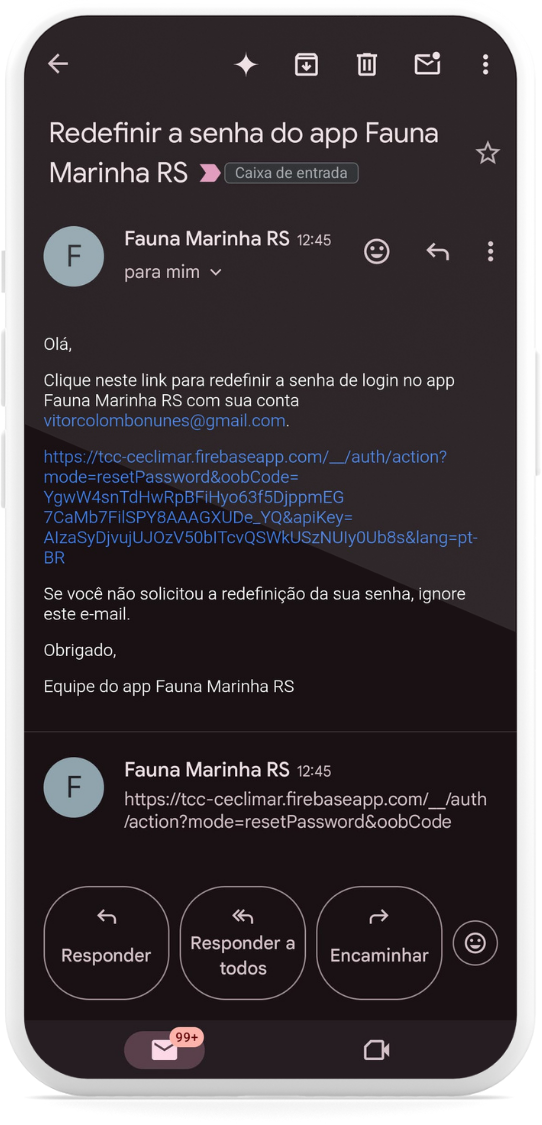
\includegraphics[height=0.72\textheight]{imagens/sistema/device_frame/emailRecSenha.png}
        \caption{E-mail personalizado de recuperação de senha.}
        \label{fig:email-esqueci-senha}
    \end{minipage}
\end{figure}
\legend{Fonte: Autor}

Para usuários que ainda não possuem uma conta, a tela de cadastro (Figura~\ref{fig:cadastro})
oferece a opção de criar uma nova conta. O cadastro é realizado por meio de um formulário com validação 
(Figura~\ref{fig:cadastro-erro}) que exige apenas dados básicos necessários para o funcionamento do sistema, 
como nome, e-mail e senha, evitando a coleta excessiva de informações pessoais conforme as diretrizes da 
LGPD \cite{BRASIL2018lgpd}. Todos os usuários criados por essa tela serão registrados inicialmente como usuários 
comuns.
A senha deve atender aos critérios de segurança, incluindo pelo menos um caractere especial, uma letra minúscula, 
uma letra maiúscula e deve possuir, no mínimo, 6 caracteres. Após o cadastro bem sucedido, o usuário 
é autenticado e redirecionado para o menu inicial da aplicação.

\begin{figure}[H]
    \centering
    \begin{minipage}[t]{0.48\textwidth}
        \centering
        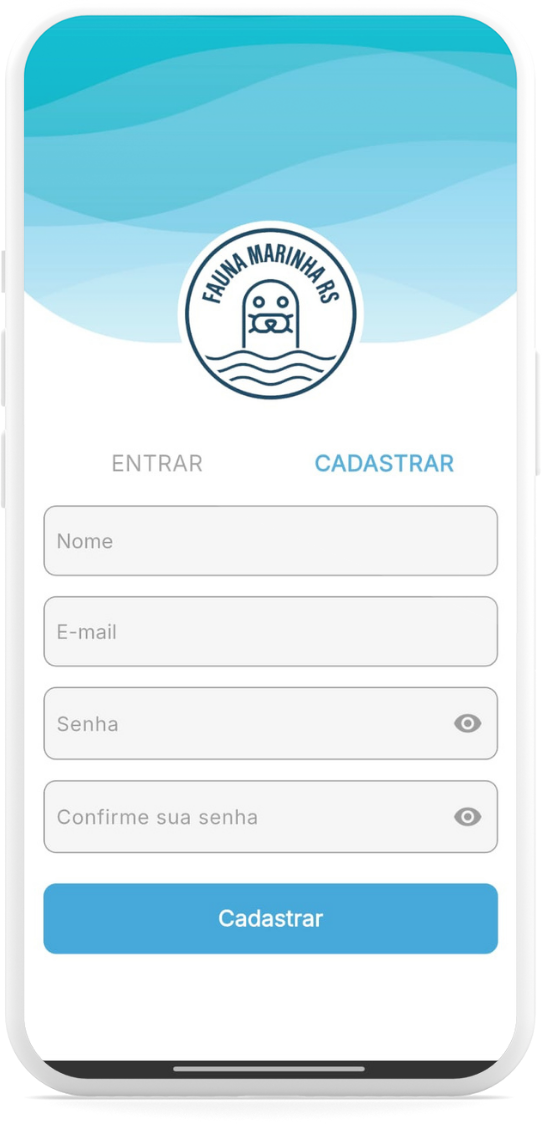
\includegraphics[height=0.72\textheight]{imagens/sistema/device_frame/cadastro.png}
        \caption{Tela de cadastro de usuário com formulário simples.}
        \label{fig:cadastro}
    \end{minipage}
    \hfill
    \begin{minipage}[t]{0.48\textwidth}
        \centering
        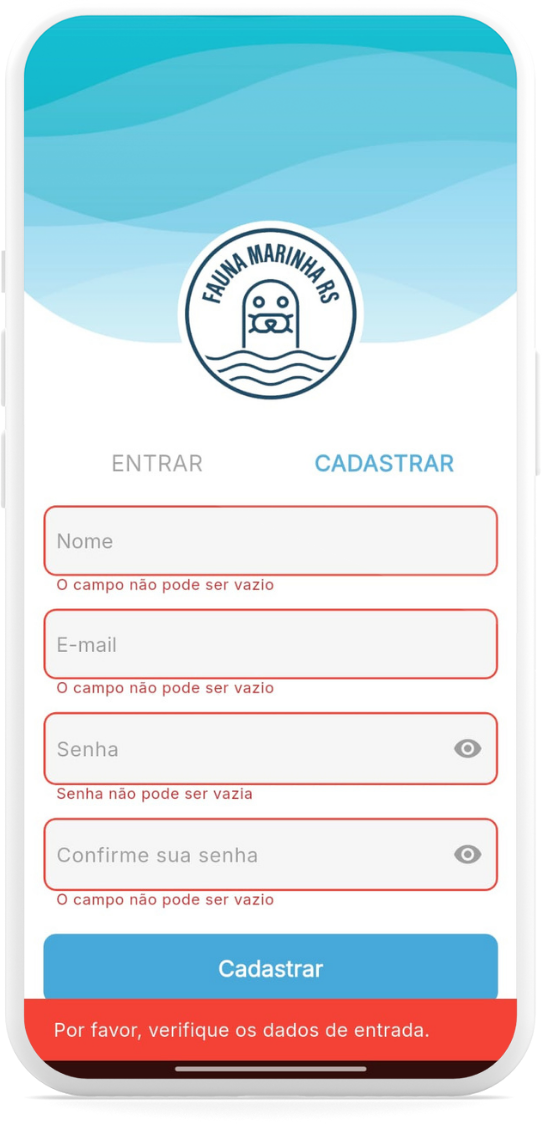
\includegraphics[height=0.72\textheight]{imagens/sistema/device_frame/formularioCadastro_erro.png}
        \caption{Exemplo de mensagens de erro na validação do formulário de cadastro.}
        \label{fig:cadastro-erro}
    \end{minipage}
\end{figure}
\legend{Fonte: Autor}

\subsection{Menu Inicial e Barra de Navegação}
Com o usuário autenticado, o aplicativo exibe o menu inicial (Figura~\ref{fig:menu-inicial-user}),
que centraliza todas as funcionalidades do sistema em um \textit{grid} 4x2. Nele estão dispostos \textit{cards} 
padronizados com o nome e ícones representativos para cada uma das funcionalidades existentes para facilitar a 
navegação do usuário. 

\begin{figure}[H]
    \centering
    \begin{minipage}[t]{0.48\textwidth}
        \centering
        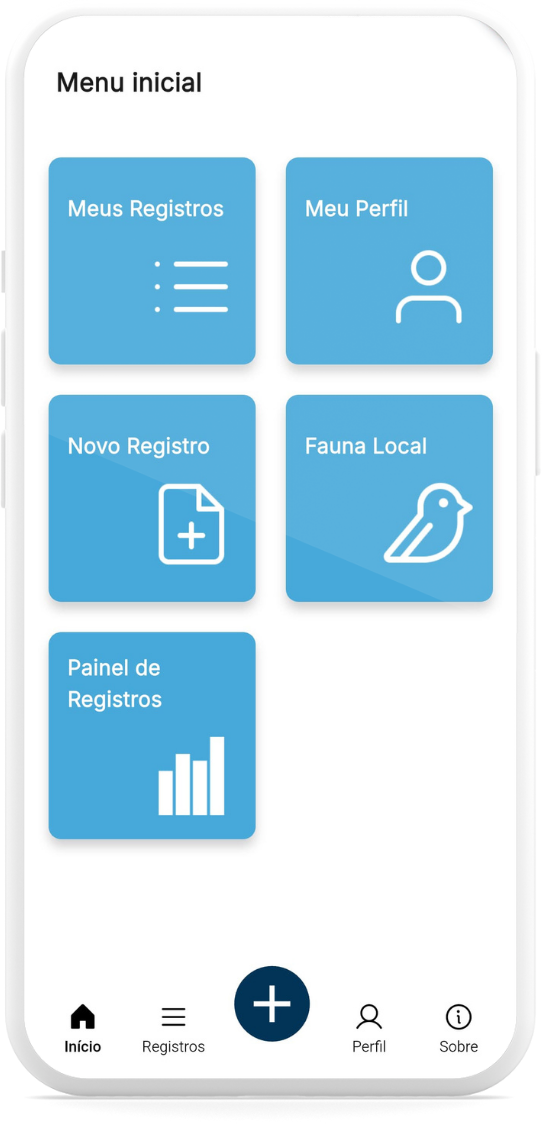
\includegraphics[height=0.72\textheight]{imagens/sistema/device_frame/menuCidadao.png}
        \caption{Tela de Menu Inicial com funcionalidades liberadas para usuários comuns.}
        \label{fig:menu-inicial-user}
    \end{minipage}
    \hfill
    \begin{minipage}[t]{0.48\textwidth}
        \centering
        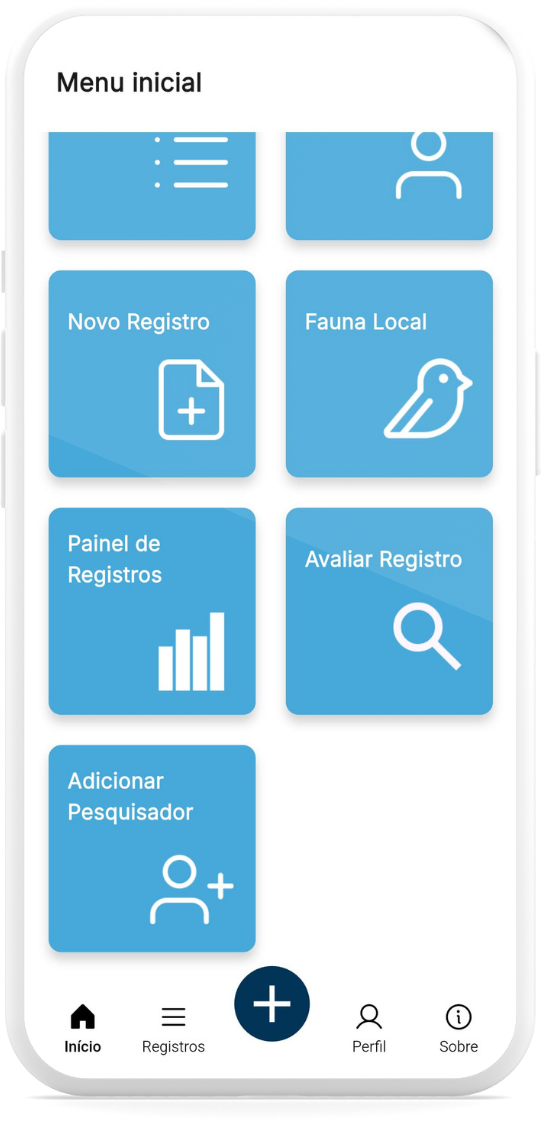
\includegraphics[height=0.72\textheight]{imagens/sistema/device_frame/menuPesquisador.png}
        \caption{Tela de Menu Inicial com funcionalidades exclusivas de pesquisadores.}
        \label{fig:menu-inicial-admin}
    \end{minipage}
\end{figure}
\legend{Fonte: Autor}

Este menu possui variações que dependem do tipo de usuário autenticado e da conexão do 
dispositivo com a internet. Se o usuário for um cientista cidadão, ele terá acesso apenas às funcionalidades 
básicas de "Meus Registros", "Meu Perfil", "Novo Registro", "Fauna Local" e "Painel de Registros".

Por outro lado, se o usuário for um pesquisador, ele terá acesso às funcionalidades adicionais 
de "Avaliar Registros" e "Adicionar Pesquisador" (Figura~\ref{fig:menu-inicial-admin}), porém essas 
funcionalidades só estarão disponíveis se o dispositivo estiver conectado à internet, 
pois dependem de acesso ao banco de dados remoto para funcionar corretamente. A Figura~\ref{fig:menu-pesq-off}
apresenta o estado do menu inicial quando essas funcionalidades estão desabilitadas. Os \textit{cards}
das funcionalidades em questão dão lugar a um outro que informa que elas estão indisponíveis por 
falta de conexão com a internet.

\begin{figure}[H]
    \centering
    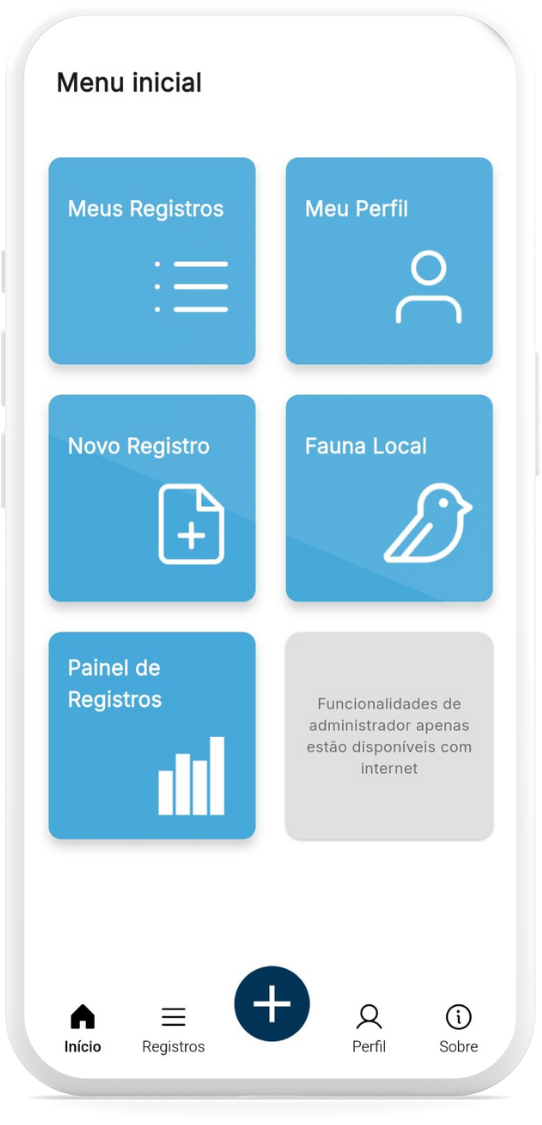
\includegraphics[height=0.72\textheight]{imagens/sistema/device_frame/menuPesquisadorOff.png}
    \caption{Tela de menu inicial com funcionalidades restritas para pesquisadores.}
    \label{fig:menu-pesq-off}
\end{figure}
\legend{Fonte: Autor}

O aplicativo apresenta também conta com uma barra de navegação inferior fixa que apenas não está presente 
nas telas de login e cadastro. Ela contém botões de acesso rápido com texto e ícones representativos de 
cada funcionalidade, permitindo que o usuário navegue facilmente entre as principais seções do aplicativo. 

A barra é composta por cinco elementos principais. O primeiro botão, da esquerda para a direita é o de 
"Início", representado por um ícone de casa, que redireciona o usuário ao "Menu Inicial" da aplicação. 
O segundo botão, "Registros", representado por um ícone de lista e leva à tela de "Meus registros". 
Centralizado na barra existe um botão flutuante com um ícone de "+", que permite que o usuário acesse 
rapidamente um formulário para envio de um registro. O quarto botão é o de "Perfil", identificado por um 
ícone de usuário ele redireciona para a tela de "Meu Perfil". E, por último, o botão "Sobre", indicado por 
um ícone de informação, redireciona para a tela de "Sobre o app".

É possível identificar em qual seção o usuário está no momento, pois o ícone se torna preenchido na coloração
preta, enquanto os demais ícones permanecem no formato vazado (Figura~\ref{fig:navbar}). 

\begin{figure}[H]
    \centering
    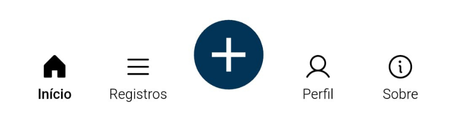
\includegraphics[width=0.7\textwidth]{imagens/sistema/device_frame/navBar.png}
    \caption{Barra de navegação fixa com o início selecionado.}
    \label{fig:navbar}
\end{figure}
\legend{Fonte: Autor}

\subsection{Meus Registros}
A tela de "Meus Registros" é onde o usuário pode visualizar todos os registros enviados por ele, 
tanto os que foram validados quanto os que ainda estão pendentes de avaliação.
Essa tela apresenta uma lista de registros que possui \textit{scroll} vertical, essa lista é populada por
registros ordenados por data de envio, do mais recente para o mais antigo, e são exibidos em blocos de
informações que incluem o nome popular do animal, a cidade onde foi avistado, a data de envio e o status de 
validação e uma imagem representativa (Figura~\ref{fig:meus-registros}).

As informações dos registros, junto com suas imagens, são baixadas do banco de dados remoto, e 
guardadas em cache local para trazer uma melhor performance na navegação do usuário e permitir que 
ele possa visualizar os registros mesmo quando estiver sem conexão com a internet.

\begin{figure}[H]
    \centering
    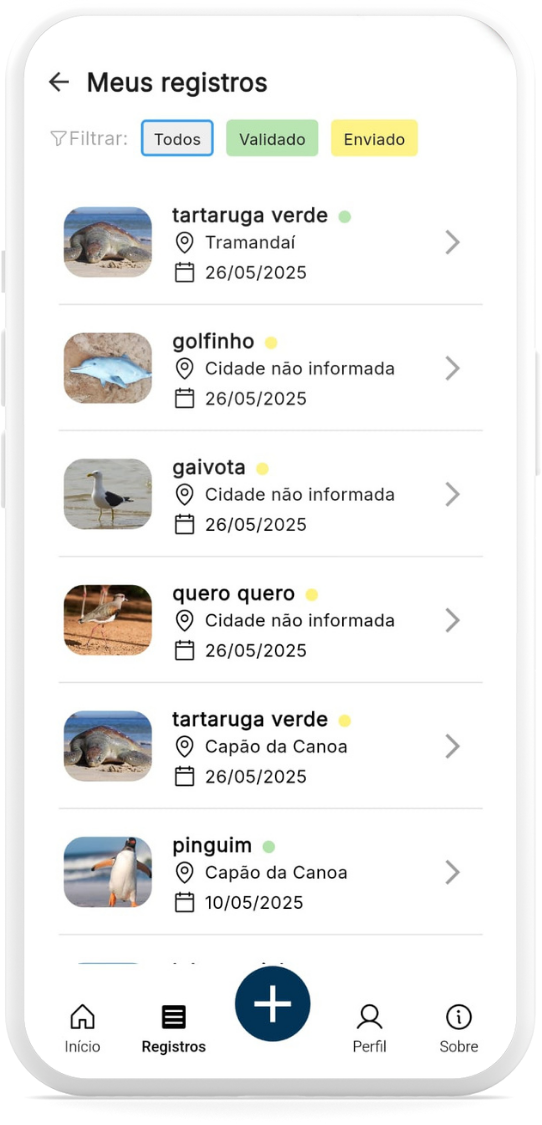
\includegraphics[height=0.72\textheight]{imagens/sistema/device_frame/meusregistrosTodos.png}
    \caption{Tela de meus registros apresentando os registros cadastrados pelo usuário em lista vertical.}
    \label{fig:meus-registros}
\end{figure}
\legend{Fonte: Autor}

Nessa tela o usuário pode realizar a filtragem dos registros baseado nos seus status de validação,
podendo escolher entre "Todos", "Validado" e "Enviado". Por padrão, a tela é carregada com o filtro de "Todos" 
selecionada e apresenta ambos os status. Porém, caso o usuário deseje, o filtro de "Validado" irá mostrar apenas
registros já foram avaliados por um pesquisador e que possuem as informações conferidas, estes são 
representados com um ponto verde ao lado do nome do animal (Figura~\ref{fig:meus-registros-validado}). 
Enquanto o filtro de "Enviado" irá apenas mostrar registros que ainda não foram avaliados, são representados 
com um ponto amarelo ao lado do nome do animal (Figura~\ref{fig:meus-registros-enviado}).

\begin{figure}[H]
    \centering
    \begin{minipage}[t]{0.48\textwidth}
        \centering
        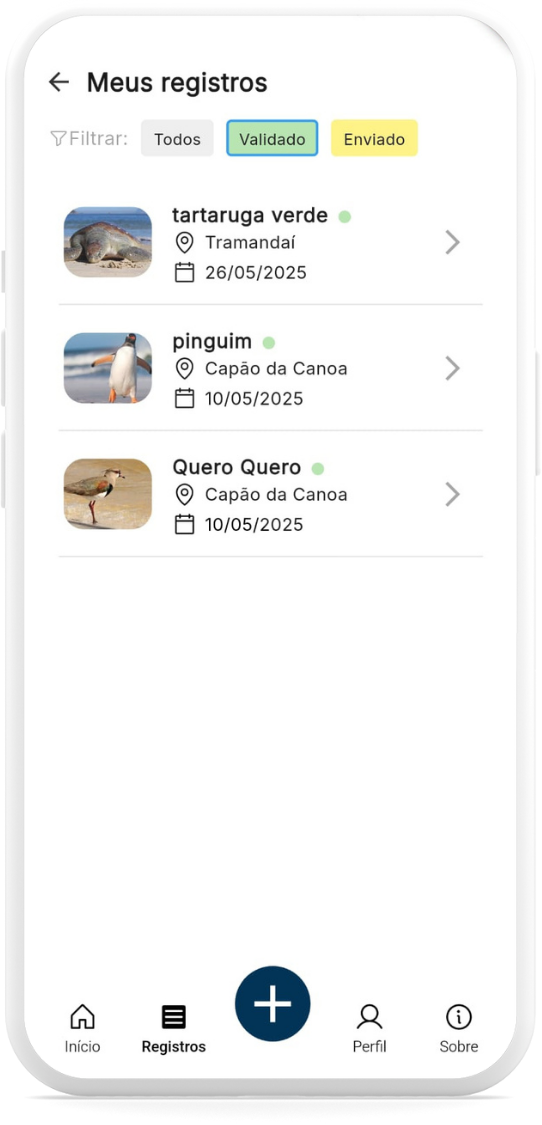
\includegraphics[height=0.72\textheight]{imagens/sistema/device_frame/meusregistrosValidado.png}
        \caption{Tela de Meus Registros com filtro de "Validado" aplicado.}
        \label{fig:meus-registros-validado}
    \end{minipage}
    \hfill
    \begin{minipage}[t]{0.48\textwidth}
        \centering
        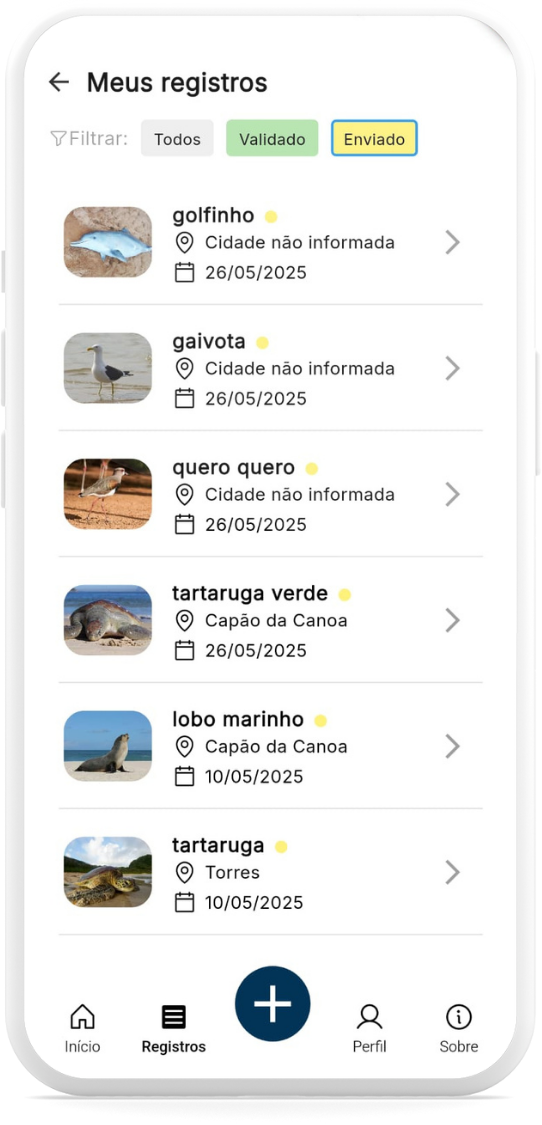
\includegraphics[height=0.72\textheight]{imagens/sistema/device_frame/meusregistrosEnviado.png}
        \caption{Tela de Meus Registros com filtro de "Enviado" aplicado.}
        \label{fig:meus-registros-enviado}
    \end{minipage}
\end{figure}
\legend{Fonte: Autor}

\subsection{Novo Registro}

\begin{figure}[H]
    \centering
    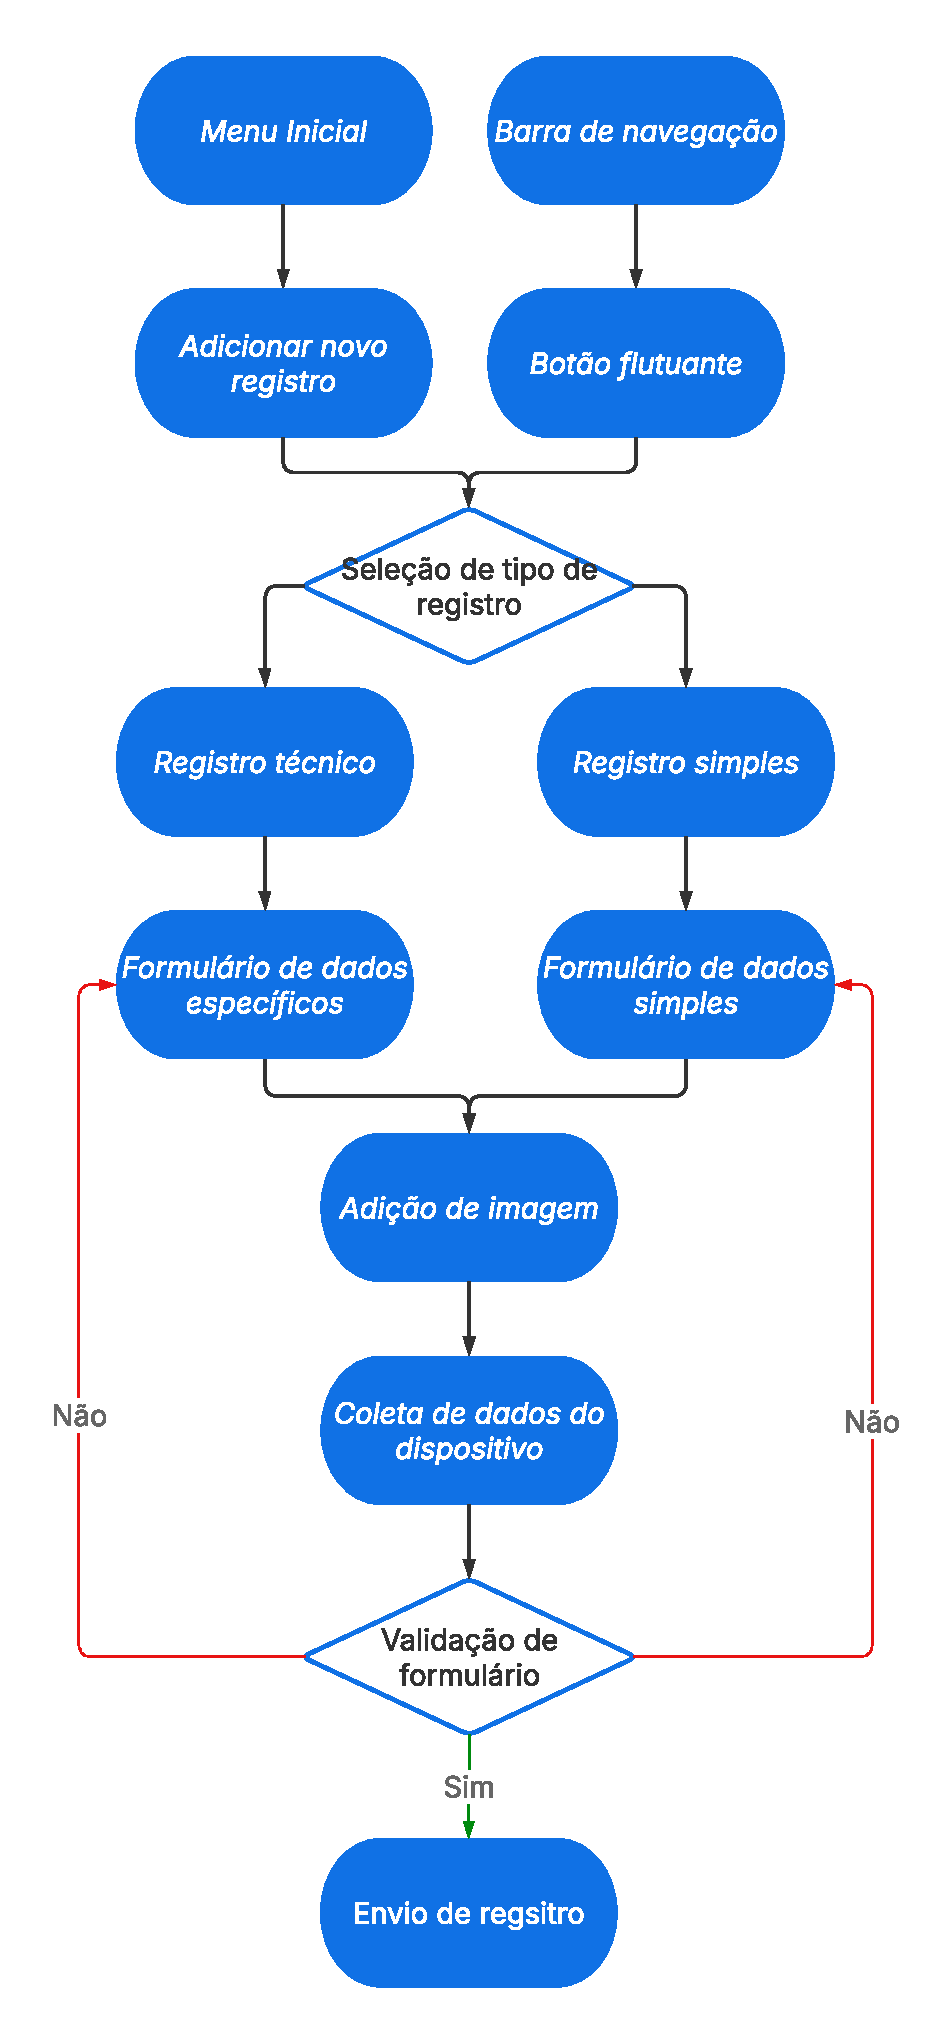
\includegraphics[height=0.90\textheight]{diagrams/fluxograma_registro.pdf}
    \caption{Fluxograma de geração de novo registro.}
    \label{fig:fluxo-novo-registro}
\end{figure}
\legend{Fonte: Autor}

\subsection{Avaliar Registro}

\begin{figure}[H]
    \centering
    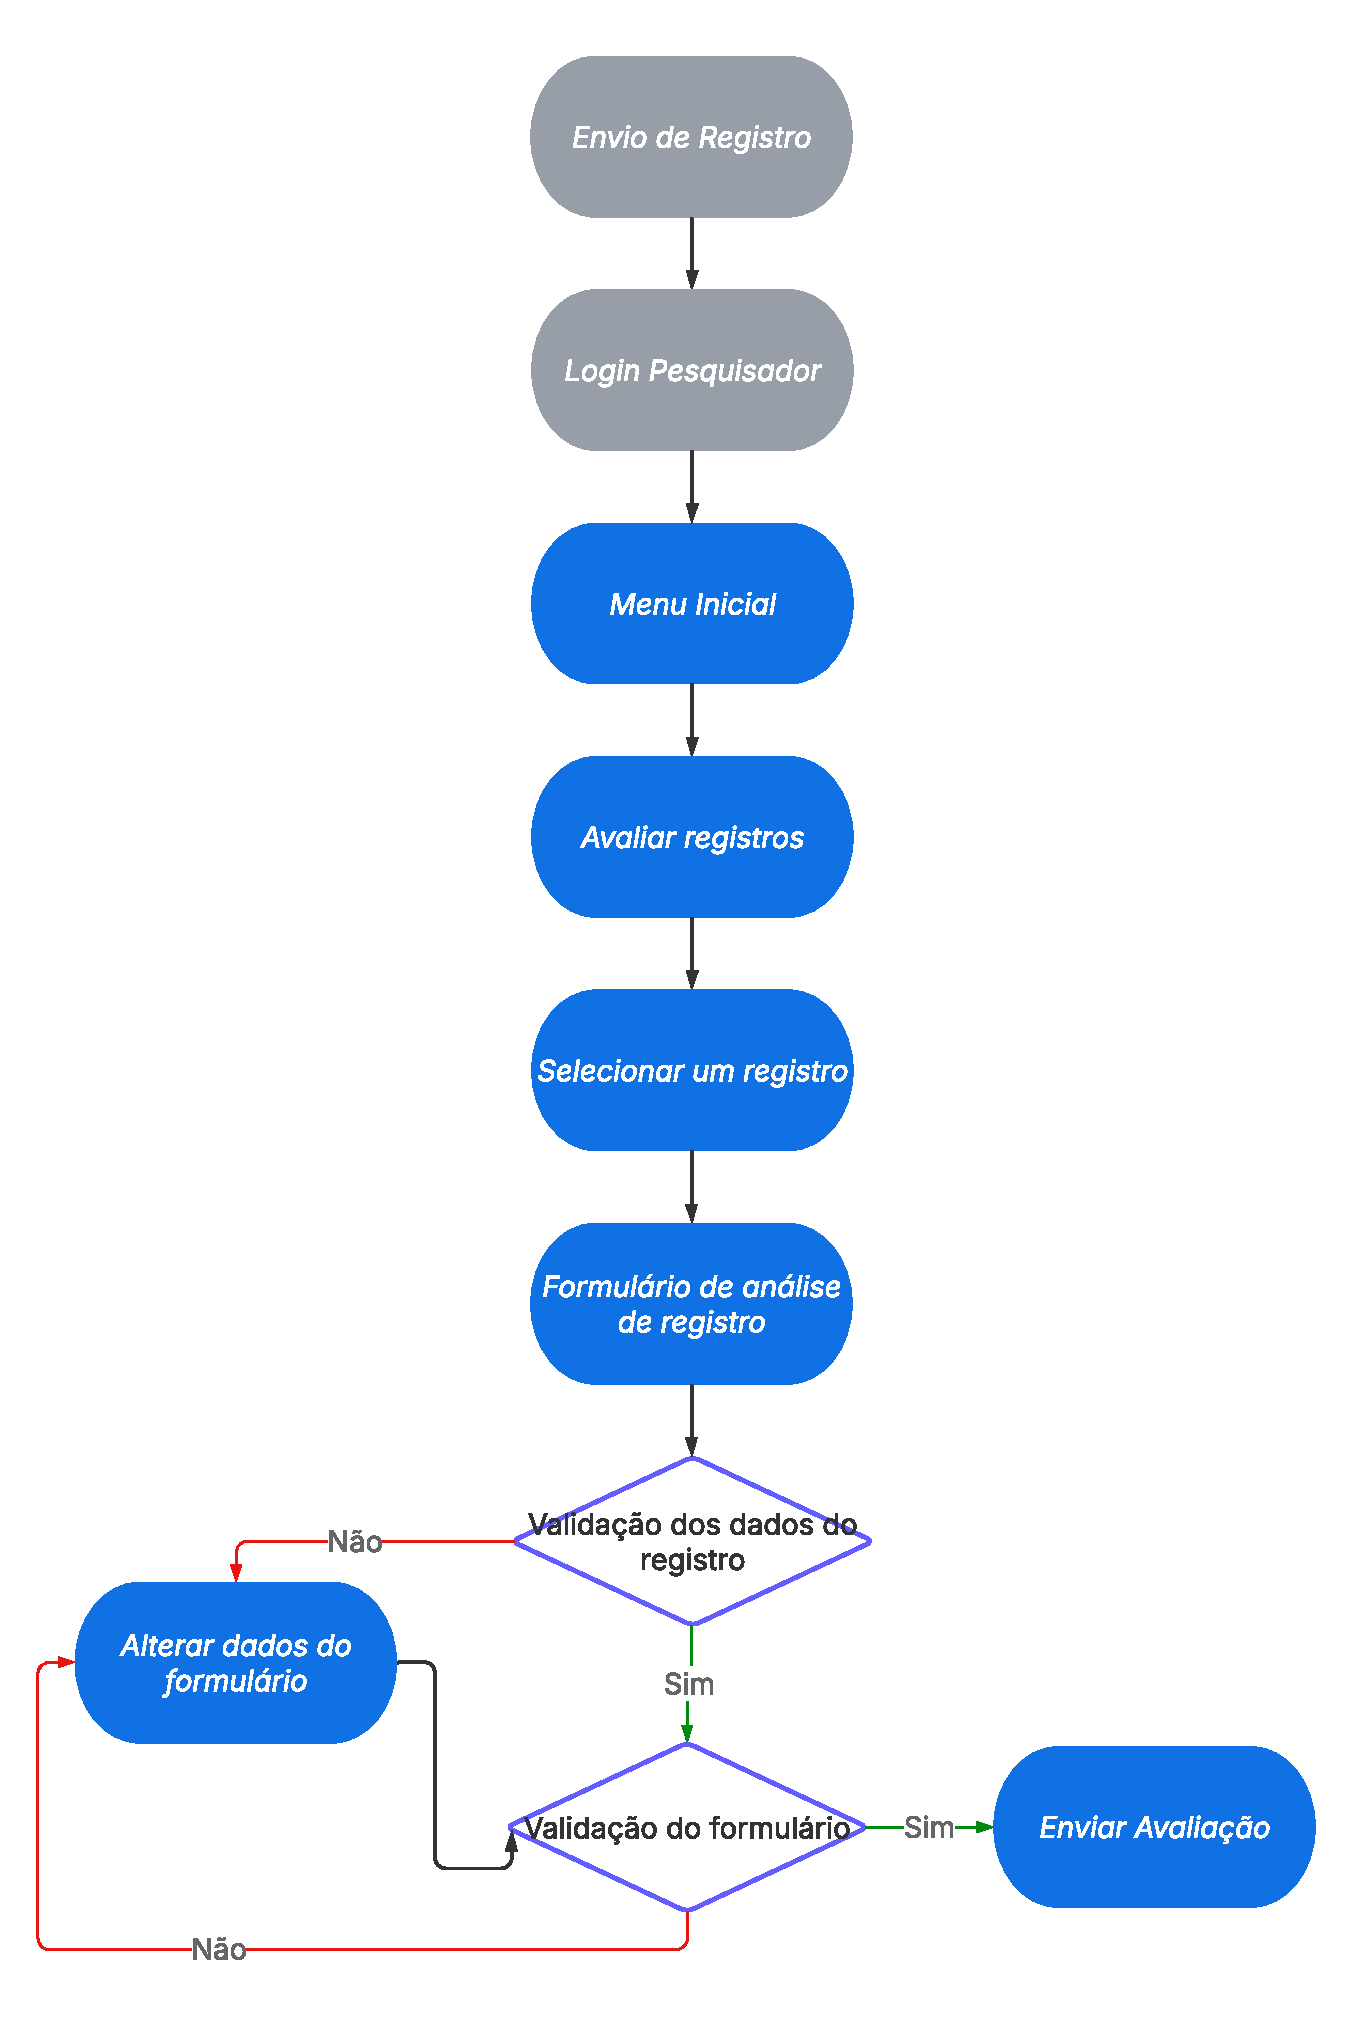
\includegraphics[height=0.90\textheight]{diagrams/fluxograma_avaliar_registro.pdf}
    \caption{Fluxograma de avaliação de registro.}
    \label{fig:fluxo-avaliar-registro}
\end{figure}
\legend{Fonte: Autor}

\subsection{Painel de Registros}

\subsection{Adicionar Pesquisador}
A funcionalidade de "Adicionar Pesquisador" é exclusiva para usuários com perfil de pesquisador e só 
está disponível quando o dispositivo está conectado à internet e permite que um pesquisador adicione 
novos usuários ao sistema com o perfil de pesquisador ou conceda permissões de pesquisador a usuários 
comuns já cadastrados. O fluxo dessa funcionalidade é apresentado na Figura~\ref{fig:fluxo-adicionar-pesquisador}.

A tela de "Adicionar Pesquisador" apresenta um formulário onde o pesquisador pode inserir o nome e o e-mail 
do usuário que deseja adicionar ou conceder a \textit{role} de pesquisador (Figura~\ref{fig:adicionar-pesquisador}).

\begin{figure}[H]
    \centering
    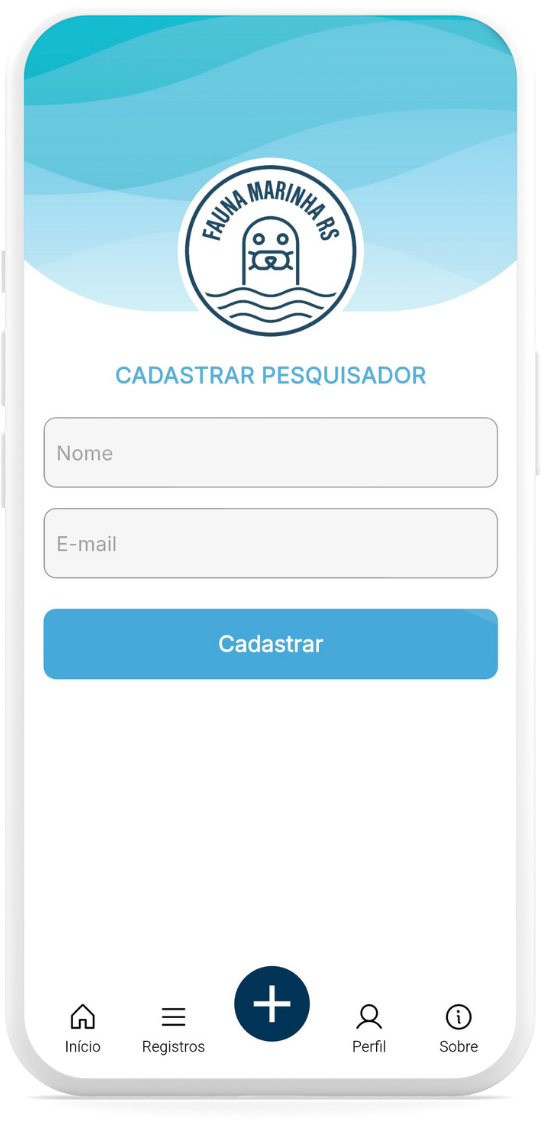
\includegraphics[height=0.7\textheight]{imagens/sistema/device_frame/cadastrarPesq.png}
    \caption{Tela de Cadastrar Pesquisador.}
    \label{fig:adicionar-pesquisador}
\end{figure}
\legend{Fonte: Autor}

\begin{figure}[H]
    \centering
    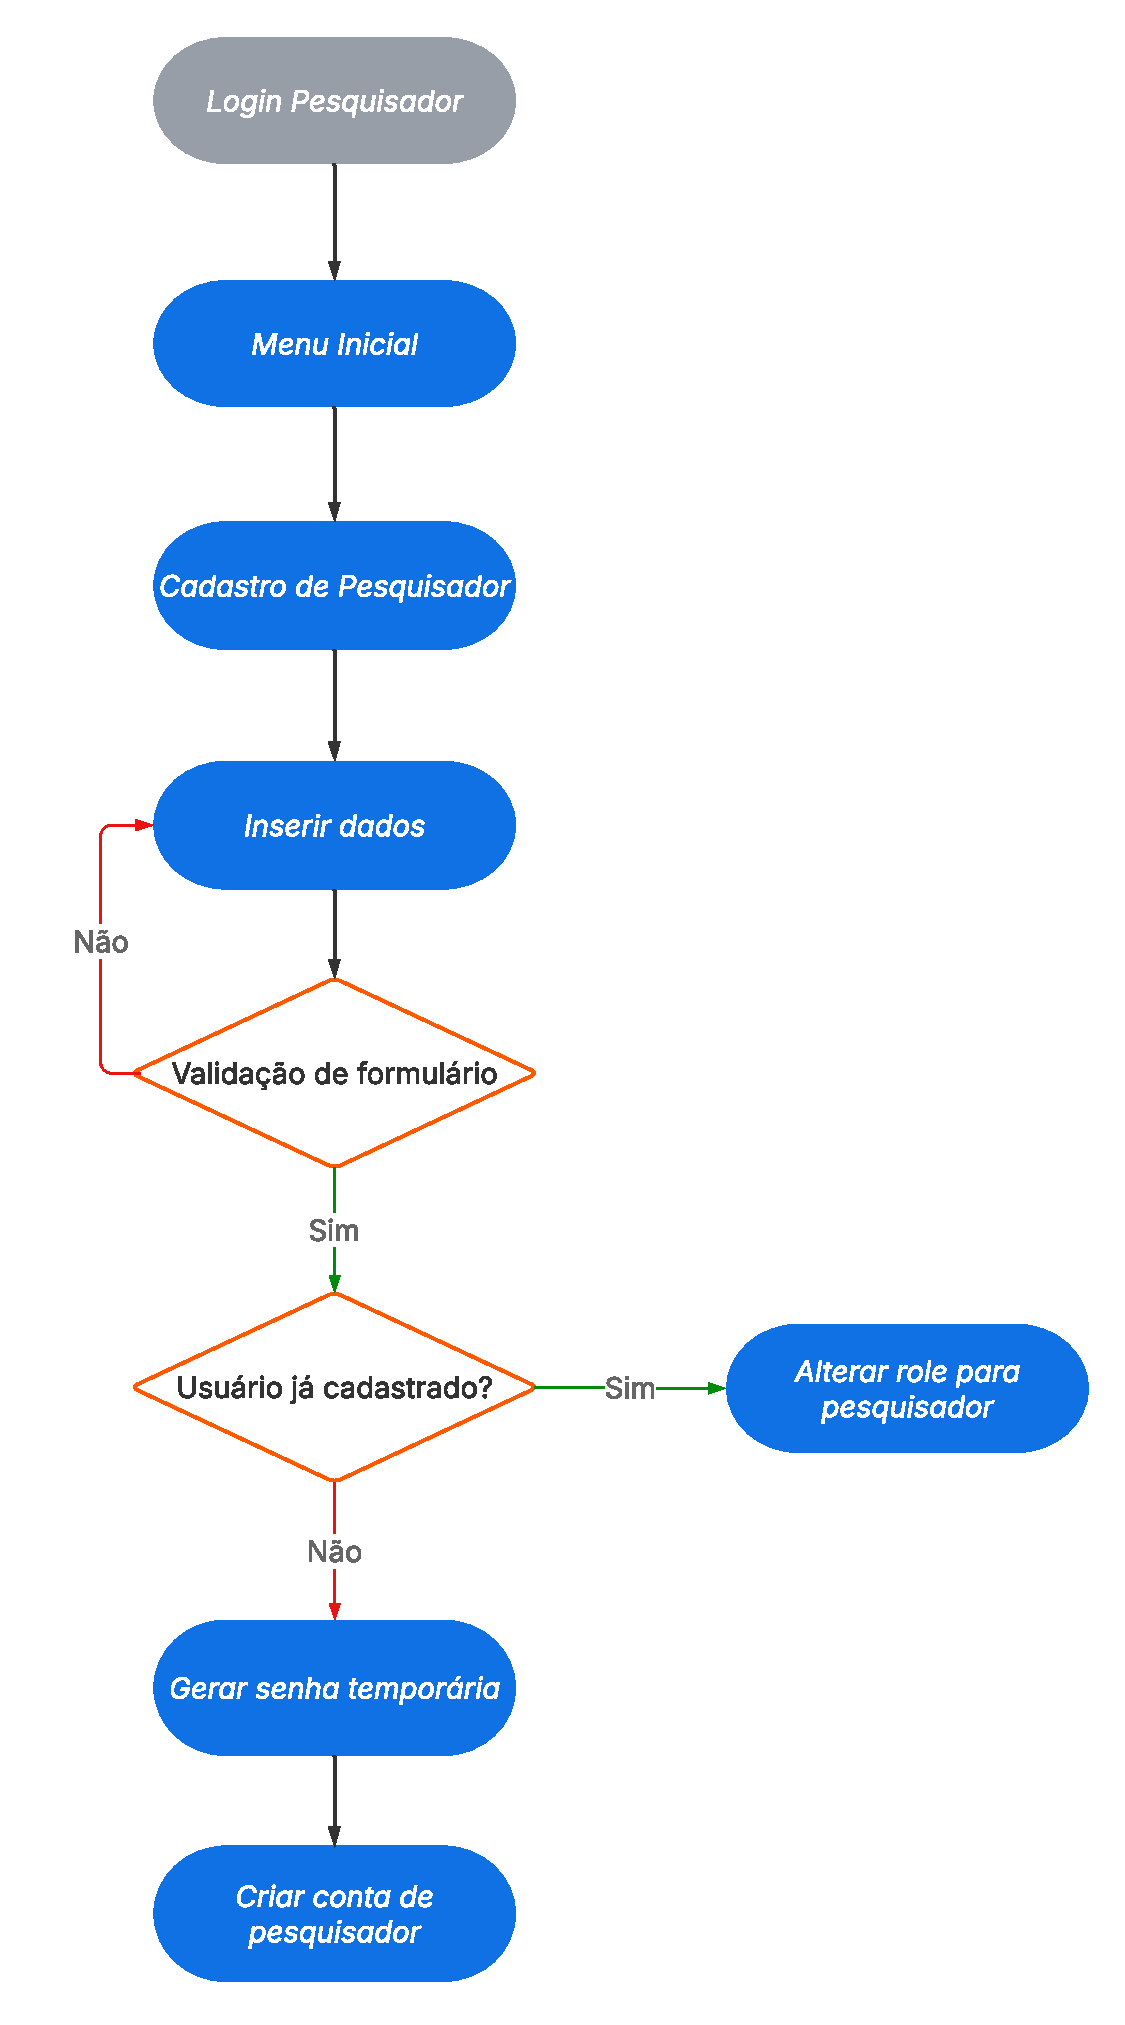
\includegraphics[height=0.90\textheight]{diagrams/fluxograma_adicionar_pesq.pdf}
    \caption{Fluxograma de adição de pesquisador.}
    \label{fig:fluxo-adicionar-pesquisador}
\end{figure}
\legend{Fonte: Autor}

Caso o usuário já esteja cadastrado no sistema, o sistema irá apresentar uma \textit{bottomsheet} informando 
que o usuário já existe e perguntará se o usuário deseja realmente conceder a \textit{role} de pesquisador para ele, caso o usuário aceite,
o sistema irá atualizar as permissões do usuário e informar que a ação foi realizada com sucesso 
(Figura~\ref{fig:cadastrarPesquisador-ja-existente}).

Caso o e-mail informado não esteja cadastrado, o sistema irá criar um novo usuário com as informações 
fornecidas e gerar uma senha temporária aleatória para ele, que será apresentada em tela com opção de 
copiar para a área de transferência (Figura~\ref{fig:cadastrarPesquisador-sucesso}).
Essa senha temporária deve ser informada pelo novo usuário ao realizar o primeiro login, onde ele poderá 
alterar a senha para uma de sua escolha.

\begin{figure}[H]
    \centering
    \begin{minipage}[t]{0.48\textwidth}
        \centering
        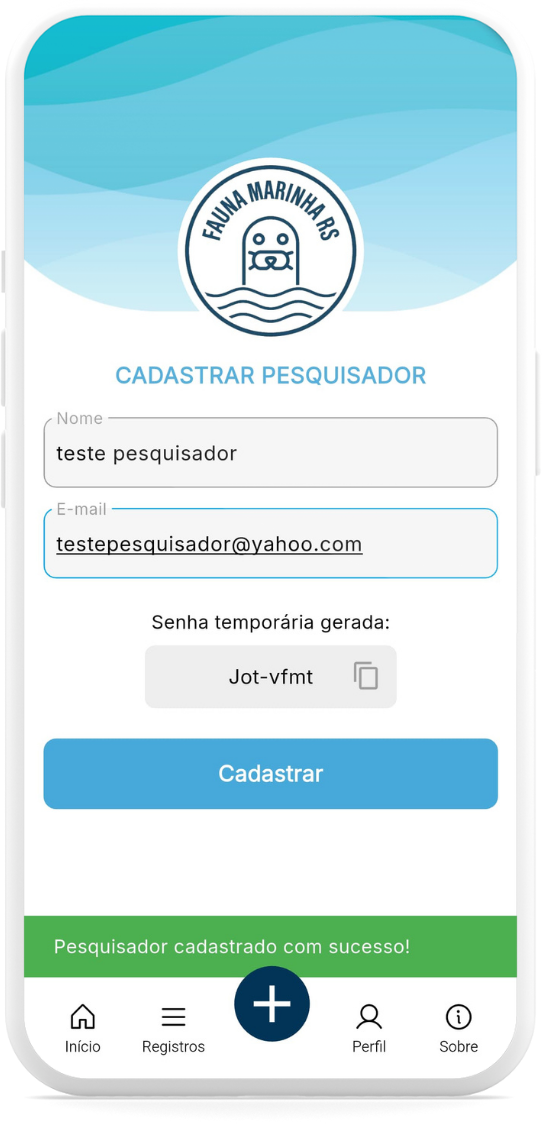
\includegraphics[height=0.72\textheight]{imagens/sistema/device_frame/cadastrarPesqSucesso.png}
        \caption{Tela de Cadastrar Pesquisador com senha aleatória gerada e mensagem de sucesso.}
        \label{fig:cadastrarPesquisador-sucesso}
    \end{minipage}
    \hfill
    \begin{minipage}[t]{0.48\textwidth}
        \centering
        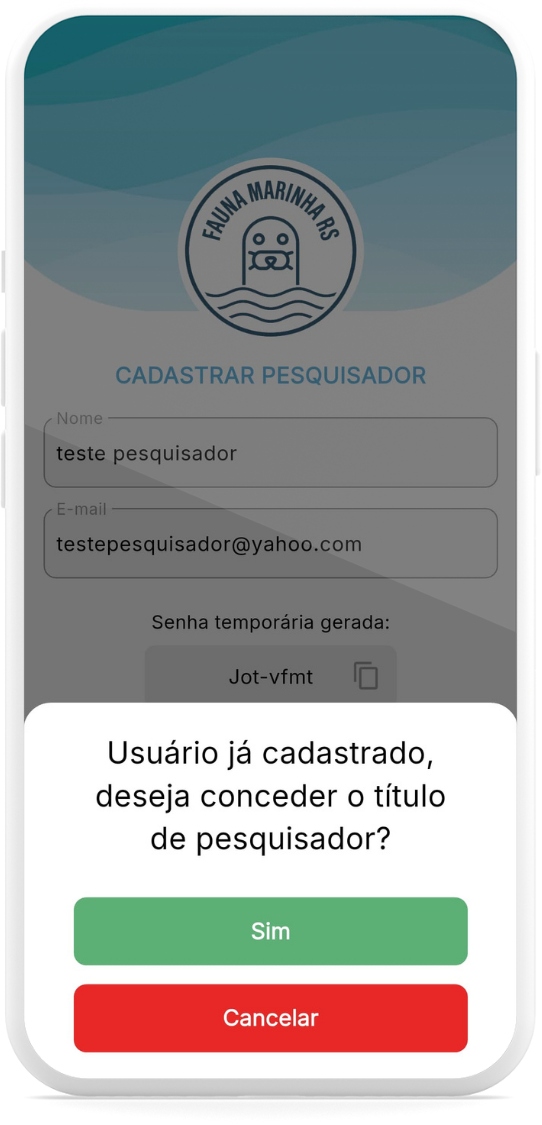
\includegraphics[height=0.72\textheight]{imagens/sistema/device_frame/cadastrarPesqJaExistente.png}
        \caption{\textit{Bottomsheet} de confirmação para conceder \textit{role} de pesquisador para o e-mail já cadastrado.}
        \label{fig:cadastrarPesquisador-ja-existente}
    \end{minipage}
\end{figure}
\legend{Fonte: Autor}

\subsection{Fauna Local}
Para a seção de fauna local, foi decidido que, em um primeiro momento,
seria utilizado o acervo externo do projeto Fauna Marinha RS, que já possui um catálogo bem documentado 
de espécies registradas no litoral gaúcho, com material didático e imagens representativas de cada espécie.
Sendo assim, o card de "Fauna Local" no menu inicial redireciona o usuário para o site do projeto 
para navegacao externa (Figura ~\ref{fig:fauna_local}).

 \begin{figure}[H]
    \centering
    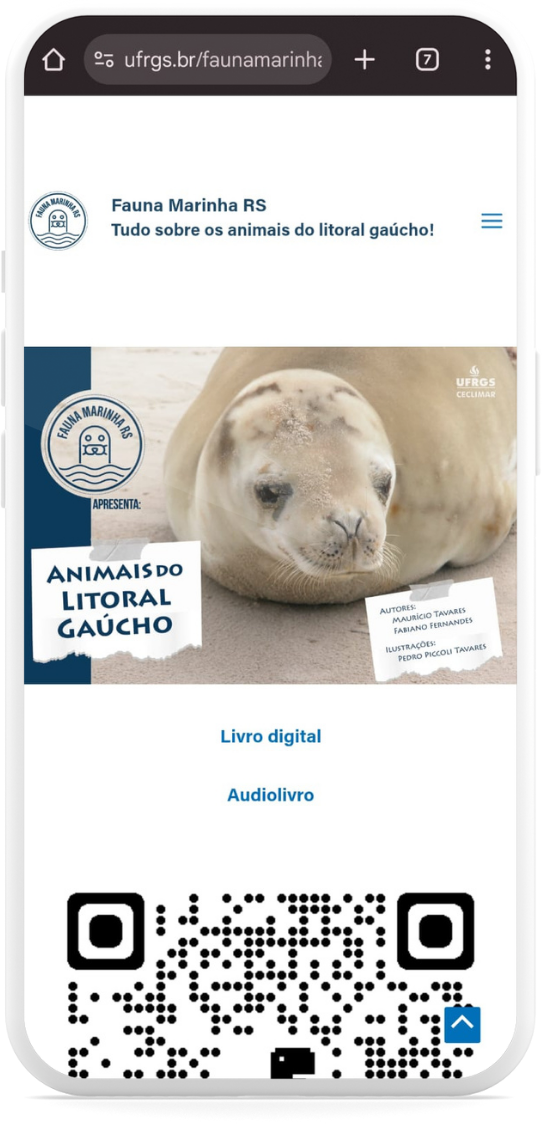
\includegraphics[height=0.7\textheight]{imagens/sistema/device_frame/faunaLocal.png}
    \caption{Tela da página de fauna local do projeto Fauna Marinha RS.}
    \label{fig:fauna_local}
\end{figure}
\legend{Fonte: Autor}


\subsection{Sobre o app}
A tela de "Sobre o app" apresenta a versão da build do aplicativo e
informações sobre o projeto Fauna Marinha RS, sobre o aplicativo e seu desenvolvimento separadas em \textit{accordions}.
Além disso, traz ícones com \textit{links} externos para as redes sociais do projeto,
como Instagram, Facebook, YouTube, Spotify, Telegram e para a caixa de e-mail, permitindo que os 
usuários acompanhem as atualizações e possam entrar em contato com a equipe do projeto (Figura~\ref{fig:sobre-app}).

\begin{figure}[H]
    \centering
    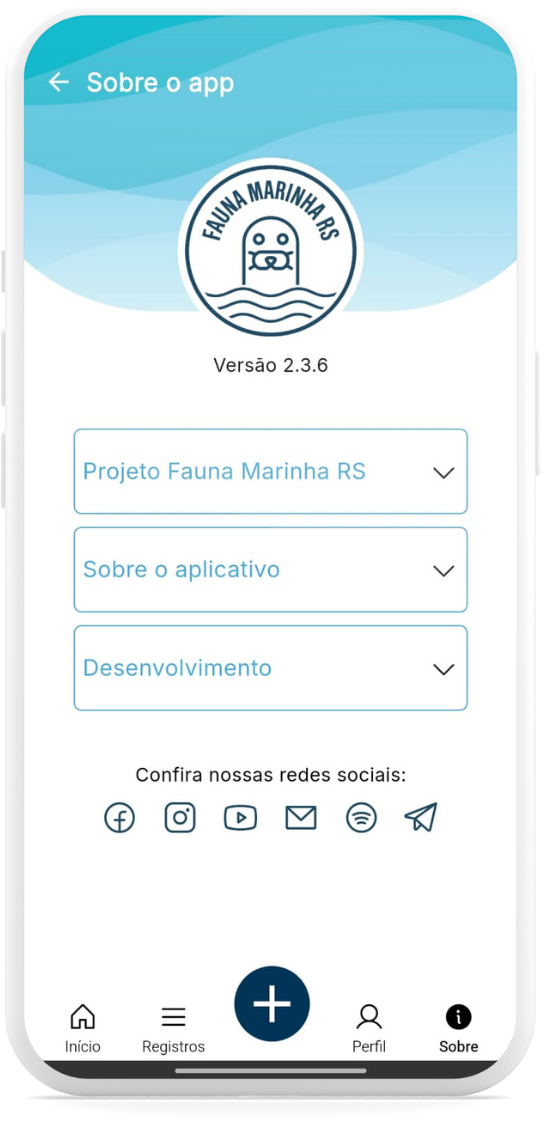
\includegraphics[height=0.7\textheight]{imagens/sistema/device_frame/sobre_app.png}
    \caption{Tela de Sobre o app, apresentando \textit{accordions} com informações do projeto e links para redes sociais.}
    \label{fig:sobre-app}
\end{figure}
\legend{Fonte: Autor}

\subsection{Armazenamento de Dados}
A estrutura do banco de dados do aplicativo foi implementada no Firebase Firestore e organizada 
em coleções com responsabilidades individuais e índices de consulta específicos para melhor performance. 

A coleção de \textit{users} armazena os dados básicos dos usuários cadastrados. 
Cada documento dessa coleção representa um usuário e cada usuário possui atrelado a ele 
uma subcoleção com seus registros (~\ref{tab:firestore-users}).
Nessa coleção, foi utilizada uma técnica de desnormalização de dados, 
onde campos como \texttt{mammalsFound}, \texttt{reptilesFound} e \texttt{birdsFound} 
são armazenados diretamente no documento do usuário, para evitar a necessidade 
de uma consulta na subcoleção de registros para obter esses dados e, posteriormente, 
atualizá-los.

Essa abordagem foi vantajosa para a funcionalidade de Meu Perfil, onde 
o usuário pode visualizar rapidamente as estatísticas de sua conta com apenas 
uma consulta ao documento do usuário.

\begin{table}[H]
    \centering
    \caption{Campos da coleção \texttt{users}}
    \label{tab:firestore-users}
    \begin{tabular}{|>{\raggedright\arraybackslash}p{3.5cm}|
                    >{\raggedright\arraybackslash}p{2cm}|
                    >{\raggedright\arraybackslash}p{7cm}|}
        \hline
        \textbf{Campo} & \textbf{Tipo} & \textbf{Descrição} \\ \hline
        \texttt{name} & string & Nome completo do usuário \\ \hline
        \texttt{email} & string & E-mail do usuário \\ \hline
        \texttt{profileImageUrl} & string & URL da imagem de perfil \\ \hline
        \texttt{createdAt} & timestamp & Data e hora de criação do perfil \\ \hline
        \texttt{role} & string & Papel do usuário no sistema \\ \hline
        \texttt{birdsFound} & number & Número de registros com aves validados que foram enviados pelo usuário \\ \hline
        \texttt{mammalsFound} & number & Número de registros com mamíferos validados que foram enviados pelo usuário \\ \hline
        \texttt{reptilesFound} & number & Número de registros com répteis validados que foram enviados pelo usuário \\ \hline
        \texttt{registers} & subcoleção & Coleção com os registros enviados pelo usuário \\ \hline
    \end{tabular}
\end{table}

A subcoleção de \textit{registers} se encontra dentro de cada documento de usuário e armazena
todos os registros enviados por aquele usuário. Cada registro é armazenado como um documento
dentro dessa subcoleção, permitindo que cada usuário tenha seus registros 
organizados de forma individualizada (Tabela~\ref{tab:subcolecao-registers}).

Essa abordagem foi adotada com o intuito de possibilitar consultas mais 
rápidas e eficientes quando o sistema precisar buscar por registros de um 
usuário específico, uma vez que o Firestore não precisará iterar sobre uma coleção 
global de registros, mas sim acessar diretamente a subcoleção pelo \texttt{path} 
\texttt{user/\{id\}/registers}, onde \texttt{\{id\}} é o ID do usuário. Essa medida também 
traz escalabilidade ao sistema, pois cada usuário terá sua própria
subcoleção de registros, e as consultas não serão afetadas pelo número 
total de registros, mas sim pelo número de registros de cada usuário individualmente.

Uma inicial desvantagem dessa abordagem seria a necessidade de realizar 
consultas para obter todos os registros do sistema já que eles estão 
distribuídos em várias subcoleções.
Porém, o Firestore oferece a funcionalidade de \textit{collection group queries},
que permite a realização de consultas em todas as subcoleções de um tipo específico.
Essa funcionalidade foi especialmente usada para implementação do painel 
de registros e avaliar registros, onde é necessário acessar
todos os registros enviados por todos os usuários.

Outro ponto onde a desnormalização foi empregada para economizar o número de 
leituras e trazer mais rapidez nas consultas foi na adição dos campos de 
\texttt{authorName} e \texttt{userId}
em cada registro, que são preenchidos automaticamente com os dados do usuário
que enviou o registro. Essa abordagem faz com que, ao listar registros para um 
usuário, não seja necessário realizar uma nova consulta no documento do usuário 
para cada item da lista.

\begin{table}[H]
    \centering
    \caption{Campos da subcoleção \texttt{users/\{id\}/registers}}
    \label{tab:subcolecao-registers}
    \begin{tabular}{|p{4cm}|p{2cm}|p{7cm}|}
        \hline
        \textbf{Campo} & \textbf{Tipo} & \textbf{Descrição} \\ \hline
        \texttt{registerNumber} & string & Número identificador único do registro \\ \hline
        \texttt{animal} & map & Dados taxonômicos do animal registrado \\ \hline
        \texttt{authorName} & string & Nome do usuário que realizou o registro \\ \hline
        \texttt{userId} & string & ID do usuário que realizou o registro (referência à coleção \texttt{users}) \\ \hline
        \texttt{date} & string & Data e hora do registro no formato ISO \\ \hline
        \texttt{location.latitude} & string & Latitude geográfica do local do registro \\ \hline
        \texttt{location.longitude} & string & Longitude geográfica do local do registro \\ \hline
        \texttt{status} & string & Status do registro \\ \hline
        \texttt{city} & string & Cidade onde ocorreu o registro \\ \hline
        \texttt{beachSpot} & string & Número da guarita \\ \hline
        \texttt{witnessed} & boolean & Indica se o animal foi testemunhado encalhando \\ \hline
        \texttt{hour} & string & Hora do encalhe \\ \hline
        \texttt{obs} & string & Observações adicionais feitas pelo usuário \\ \hline
        \texttt{referencePoint} & string & Ponto de referência \\ \hline
        \texttt{registerImageUrl} & string & URL da imagem principal do animal \\ \hline
        \texttt{registerImageUrl2} & string & URL de uma imagem adicional \\ \hline
        \texttt{sampleState} & number & Estado de decomposição do animal \\ \hline
        \texttt{specialistReturn} & string & Retorno de um especialista \\ \hline
    \end{tabular}
\end{table}
\legend{Fonte: Autor}

Além dos índices padrão criados pelo Firestore para os 
campos utilizados em filtros (\textit{where}) e ordenações (\textit{orderBy}),
foram criados índices personalizados para a subcoleção registers, com o 
objetivo de garantir melhor desempenho em consultas específicas e operações 
de filtragem. Esses índices incluem:

\begin{itemize}
    \item \texttt{register.animal.species}: para habilitar buscas por espécie de animal dentro da 
    estrutura do objeto animal. Permitindo identificar todos os registros de uma determinada
    espécie.
    \item \texttt{register.date}: para habilitar buscas de registros ordenados por data em ordem 
    crescente ou decrescente, auxiliando na exibição de listas de registros.
    \item \texttt{register.registerNumber}: para permitir buscas por número de registro, possibilitando 
    uma consulta rápida de um registro específico.
\end{itemize}

A coleção de \textit{animals} armazena informações sobre as espécies de animais
registradas no sistema, incluindo dados taxonômicos e imagens representativas de cada espécie (Tabela~\ref{tab:firestore-animals}).
Essa coleção é utilizada para fornecer informações detalhadas sobre as espécies
e para gerar uma padronização nas avaliações dos registros.

Os dados inicialmente inseridos nessa coleção são provenientes de materiais internos fornecidos
pelo CECLIMAR e são utilizados no sistema como carga para os inputs de seleção 
dos campos taxonômicos nos formulários de envio e avaliação de registros.
O sistema também permite que novos animais sejam adicionados à coleção
por pesquisadores, caso uma espécie nova seja encontrada e não esteja presente
na base de dados. 

\begin{table}[H]
    \centering
    \caption{Campos da coleção \texttt{animals}}
    \label{tab:firestore-animals}
    \begin{tabular}{|>{\raggedright\arraybackslash}p{3.5cm}|
                    >{\raggedright\arraybackslash}p{2cm}|
                    >{\raggedright\arraybackslash}p{7cm}|}
        \hline
        \textbf{Campo} & \textbf{Tipo} & \textbf{Descrição} \\ \hline
        \texttt{id} & number & Identificador do animal \\ \hline
        \texttt{popularName} & string & Nome popular da espécie \\ \hline
        \texttt{scientificName} & string & Nome científico da espécie \\ \hline
        \texttt{class} & string & Classe taxonômica \\ \hline
        \texttt{order} & string & Ordem taxonômica \\ \hline
        \texttt{family} & string & Família taxonômica \\ \hline
        \texttt{genus} & string & Gênero taxonômico \\ \hline
        \texttt{species} & string & Espécie taxonômica \\ \hline
        \texttt{quantity} & number & Quantidade de vezes que a espécie foi identificada em registros \\ \hline
        \texttt{imageUrl} & string & URL de imagem da espécie \\ \hline
    \end{tabular}
\end{table}

A coleção de \textit{counters} é utilizada para armazenar contadores gerais 
do sistema, como o número total de registros feitos e o número total de 
espécies cadastradas (Tabela~\ref{tab:firestore-counters}).

\begin{table}[H]
    \centering
    \caption{Campos da coleção \texttt{counters}}
    \label{tab:firestore-counters}
    \begin{tabular}{|>{\raggedright\arraybackslash}p{6cm}|
                    >{\raggedright\arraybackslash}p{2cm}|
                    >{\raggedright\arraybackslash}p{5cm}|}
        \hline
        \textbf{Campo} & \textbf{Tipo} & \textbf{Descrição} \\ \hline
        \texttt{registerCounter.count} & number & Contador total de registros feitos no sistema \\ \hline
        \texttt{animalCounter.generalCounter} & number & Contador total de espécies cadastradas \\ \hline
    \end{tabular}
\end{table}

\section{Execução de Testes e Verificação de Qualidade}

% Descrever testes, citar testadores, resultados dos testes e estratégias futuras.
% incluir gráficos representativos trazendo resultados dos testes e relacionar com 
% cards gerados para o Jira

\section*{Considerações Finais}

O capítulo consolidou os resultados até aqui obtidos, alinhando-os ao planejamento inicial do projeto, garantindo rastreabilidade entre requisitos, projeto e implementação.
